\documentclass[oneside]{tudelft-report}
\usepackage[justification=centering]{caption}
\usepackage{xcolor}
\usepackage{multirow}
\usepackage[numbers]{natbib}
%\usepackage{unsrtnat}
%\usepackage[numbers]{natbib}
\usepackage{epstopdf}
\usepackage{titlesec}
\usepackage{float}
\usepackage{todonotes}
\usepackage{comment}
\setcounter{secnumdepth}{3}
\setcounter{tocdepth}{3}
%%Abbreviation and                                      
%\documentclass{standalone}
\usepackage{tikz}
\usepackage{PTSansNarrow}
\usepackage[T1]{fontenc}
\usepackage{pdfpages} %nived's pdf package
%\usepackage{changes}
%\chapterfont{\color{blue}}
%\sectionfont{\color{blue}}
%\subsectionfont{\color{blue}}


\usepackage[colorlinks=true, allcolors=cyan]{hyperref}

\usetikzlibrary{matrix}
\usepackage[dvipsnames]{xcolor}
\usepackage{notoccite}

%nomenclature
\usepackage{changes}  
\usepackage{caption}            %%To adjust captions
\usepackage{anyfontsize}        %%To change font sizes
\usepackage{soul}               %%To highlight text
\usepackage{hyperref}       %% To link external websites to the word
\usepackage{lettrine}       %To make the first letter big
\usepackage[export]{adjustbox}  %%To move images left/right
\usepackage{graphicx}       %% To add images
\usepackage{wrapfig}        %%To add wrapped figures
\usepackage[utf8]{inputenc} %% For quotation mark
% \usepackage{dirtytalk}      %% For quotation mark
% \usepackage{subcaption}     %%For adding multiple subimages in an image
\usepackage{float}
\usepackage{booktabs}
\usepackage{doi}
\usepackage{geometry}
\usepackage[labelformat=simple]{subcaption}
\renewcommand\thesubfigure{(\alph{subfigure})}
\usepackage{amssymb}
\usepackage{amsmath}        %%To add equations
\usepackage{bm}             %%To use bold symbols in math mode
\usepackage{siunitx}        %% For proper display of numbers with SI units
\sisetup{obeyall}
\sisetup{detect-weight=true, detect-family=true}    %% To have bold in text
\usepackage{eurosym}        %% TO use euro symbol
\numberwithin{equation}{chapter}
% \usepackage{siunitx} % Required for numbers alignment in tables
% \sisetup{
%   round-mode          = places, % Rounds numbers
%   round-precision       = 2, % to 2 places
% }
\usepackage{lastpage}
\usepackage{fancyhdr}
\pagestyle{fancy} 

\usepackage{enumitem}
%\cfoot{\thepage\ of \pageref{LastPage}}

%usepackage[acronym]{glossaries}
%\makeglossaries
\usepackage[nonumberlist,acronym]{glossaries}
\makeglossaries
\usepackage[toc,page]{appendix}
\newglossaryentry{RES}{name={RES},description={Renewable Energy Sources}}
\newglossaryentry{VSC}{name={VSC},description={Voltage Source Converter}}
\newglossaryentry{MSC}{name={MSC}, description={Machine Side Converter}}
\newglossaryentry{GSC}{name={GSC}, description={Grid Side Converter}}
\newglossaryentry{LSC}{name={LSC}, description={Line Side Converter}}
\newglossaryentry{MMC}{name={MMC}, description={Modular Multi-level Converter}}
\newglossaryentry{AC}{name={AC}, description={Alternating Current}}
\newglossaryentry{DC}{name={DC}, description={Direct Current}}
\newglossaryentry{EMF}{name={EMF}, description={Electromotive Force}}
\newglossaryentry{PMSG}{name={PMSG}, description={Permanent Magnet Synchronous Generator}}
\newglossaryentry{OWF}{name={OWF}, description={Offshore Wind Farm}}
\newglossaryentry{WG}{name={WG}, description={Wind Generator}}
\newglossaryentry{WT}{name={WT}, description={Wind Turbine}}
\newglossaryentry{HVAC}{name={HVAC}, description={High Voltage Alternating Current}}
\newglossaryentry{HVDC}{name={HVDC}, description={High Voltage Direct Current}}
\newglossaryentry{CB}{name={CB}, description={Circuit Breaker}}
\newglossaryentry{PE}{name={PE}, description={Power Electronic}}
\newglossaryentry{VCO}{name={VCO}, description={Voltage Controlled Oscillator}}
\newglossaryentry{DVC}{name={DVC}, description={Direct Voltage Control}}
\newglossaryentry{FOC}{name={FOC}, description={Field Oriented Control}}
\newglossaryentry{DTC}{name={DTC}, description={Direct Torque Control}}
\newglossaryentry{Hcosnti}{name={H}, description={Inertia Constant}}
\newglossaryentry{FAPR}{name={FAPR}, description={Fast Active Power Regulation}}
\newglossaryentry{EU}{name={EU}, description={European Union}}
\newglossaryentry{PCC}{name={PCC}, description={Point of Common Coupling}}
\newglossaryentry{HPF}{name={HPF}, description={High Pass Filter}}
\newglossaryentry{PLL}{name={PLL}, description={Phase Locked Loop}}
\newglossaryentry{LVRT}{name={LVRT}, description={Low Voltage Right Through}}
\newglossaryentry{PEIG}{name={PEIG}, description={Power Electronic Interfaced Generation}}
\newglossaryentry{EMT}{name={EMT}, description={Electromagnetic Transient}}
\newglossaryentry{NPC}{name={NPC}, description={Neutral Point Clamped}}
\newglossaryentry{MPPT}{name={MPPT}, description={Maximum Power Point Tracking}}
\newglossaryentry{WECS}{name={WECS}, description={Wind Energy Conversion Systems}}
\newglossaryentry{THD}{name={THD}, description={Total Harmonic Distortion}}
\newglossaryentry{PI}{name={PI}, description={Proportional Integral}}
\newglossaryentry{IGBT}{name={IGBT}, description={Insulated Gate Bipolar Transistors}}
\newglossaryentry{PWM}{name={PWM}, description={Pulse Width Modulation}}
\newglossaryentry{HV}{name={HV}, description={High Voltage}}
\newglossaryentry{LV}{name={LV}, description={Low Voltage}}
\newglossaryentry{dq}{name={dq}, description={Direct Quadrature}}
\newglossaryentry{RTDS}{name={RTDS}, description={Real Time Digital Simulator}}
\newglossaryentry{VDAPR}{name={VDAPR}, description={Voltage Dependent Active Power Reduction}}
\newglossaryentry{FSC}{name={FSC}, description={Full scale converter}}

\glstoctrue


\begin{document}



%% Use Roman numerals for the page numbers of the title pages and table of
%% contents

\frontmatter

\title{Development of a Generic Model for Real-time Simulation and Assessment of the Dynamic Performance of a Large Scale Offshore Transmission Network}
%\coverimage{cover.jpg}

\author{Saran Ganesh}
%\affiliation{Technische Universiteit Delft}
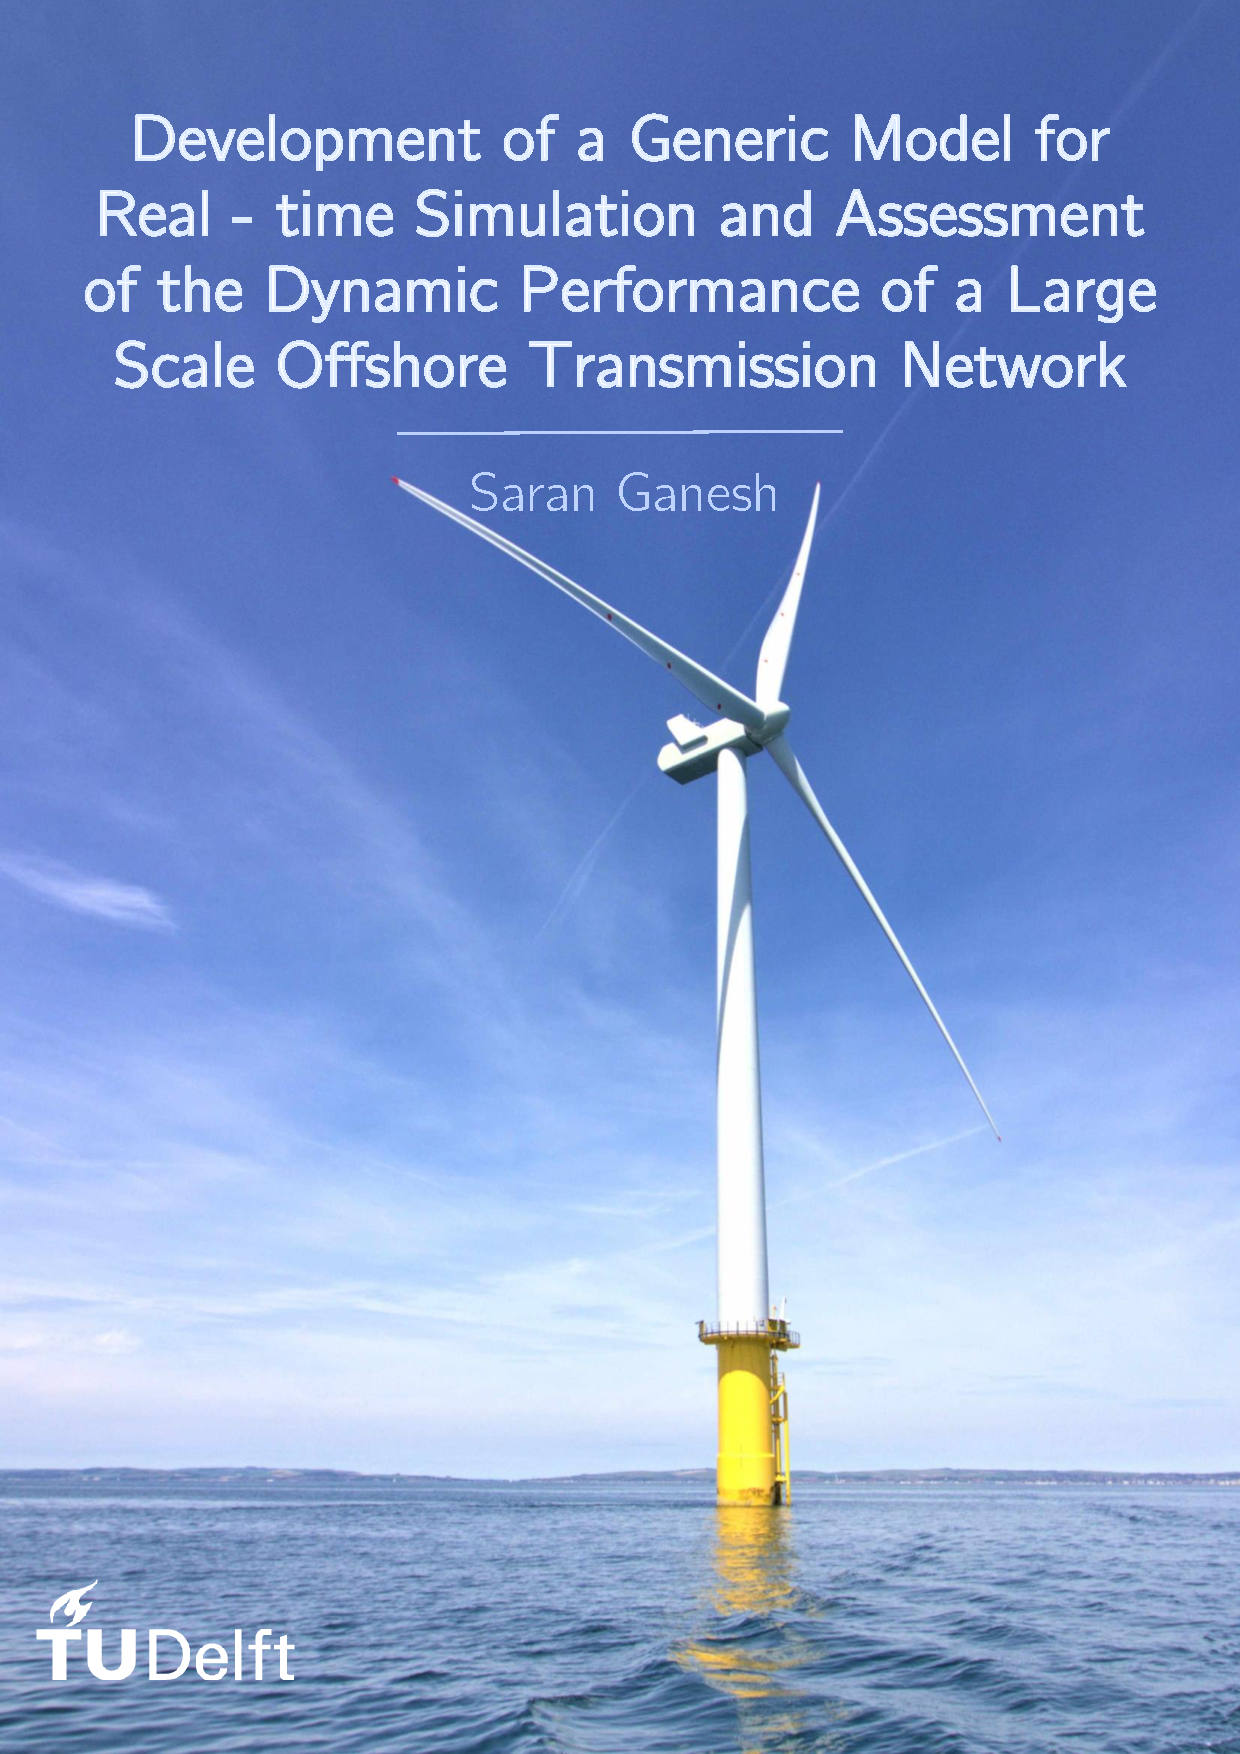
\includepdf{Saran_cover_diff_color_newmargin.pdf}
%\makecover

%% Include an optional title page.
\begin{titlepage}

\begin{center}

%% Insert the TU Delft logo at the bottom of the page.
\begin{tikzpicture}[remember picture,overlay]
    \node at (current page.south)[anchor=south,inner sep=0pt]{
        
\includegraphics{cover/logo}
    };
\end{tikzpicture}

%% Extra whitespace at the top.
\vspace*{2\bigskipamount}

%% Print the title in cyan.
{\makeatletter
\titlestyle\color{tudelft-cyan}\Huge\@title
\makeatother}

%% Print the optional subtitle in black.
{\makeatletter
\ifx\@subtitle\undefined\else
    \bigskip
    \titlefont\titleshape\Huge\@subtitle
\fi
\makeatother}

\bigskip
\bigskip

by
%door

\bigskip
\bigskip

%% Print the name of the author.
{\makeatletter
\titlefont\Huge\bfseries\@author
\makeatother}

\vfill

in partial fulfillment of the requirements for the degree of
%in overeenstemming met de vereisten voor het verkrijgen van de graad van

\bigskip
\bigskip

{\bfseries Master of Science}

in Electrical Power Engineering

\bigskip
\bigskip

at the Delft University of Technology,
%aan de Technische Universiteit Delft,

to be defended on October 29, 2020 at 10:00 AM.
%in het openbaar de verdedigen op dinsdag 1 januari om 10:00 uur.

\vspace{25mm}

\begin{tabular}{lll}
%% Add additional information here, per faculty requirements, e.g
%    Student number: & 1234567 \\
%    Project duration: & \multicolumn{2}{l}{March 1, 2012 -- January 1, 2013} \\
    Supervisor: & Dr.\ ir.\ J.L.\ (Jose) Rueda Torres \\
    Thesis committee:
        & Prof.\ ir.\ M.A.M.M.\ (Mart) van der Meijden, & IEPG\\
        & Dr.\ ir.\ J.L.\ (Jose) Rueda Torres, & IEPG  \\
        & Dr.\ T.\ (Thiago) Batista Soeiro & DCES \\
        
\end{tabular}

\vspace{35mm}
%% Only include the following lines if confidentiality is applicable.
\bigskip
\emph{This thesis is confidential and cannot be made public until December 31, 2022.}
%\emph{Op dit verslag is geheimhouding van toepassing tot en met 31 december 2013.}

\bigskip

An electronic version of this thesis is available at \url{http://repository.tudelft.nl/}.
%Een elektronische versie van dit verslag is beschikbaar op \url{http://repository.tudelft.nl/}.
\vspace{15mm}
\end{center}

\end{titlepage}



\chapter*{Acknowledgement}

There are many people to thank for the successful completion of this project. Firstly, I would like to thank Dr. Jose Rueda Torres for providing me this opportunity to work on such an interesting topic and guiding me throughout the research. His inputs and suggestions throughout the thesis have been extremely valuable. All the constructive criticisms have contributed to developing me as a good researcher and a good human being. I also would like to thank Prof. Mart van der Meijden for his suggestions and constant support through several meetings. He has always taken keen interest in letting me develop my skills and made me aware of the bigger picture of the work I was doing. I am incredibly thankful to both my supervisors for their support and goodwill during this thesis. 


I would like to extend my thanks to Arcadio Perilla for kindly consenting to be a part of my defense committee.
I cannot thank enough my daily supervisor İlker Tezsevin. He has been a constant support and a pillar of strength throughout my thesis project and internship. This thesis would not have been possible without his help and contribution. He has been a great teacher to me from the start of my internship project at DIFFER. His determination and motivation to work have always made an impact on me. I am sure that this learning experience I had from him will be an asset to me. On a lighter note, I will never forget these two things: first, our discussions after coming out of meetings with Suleyman! And his expression whenever I say I have a new idea!
A huge thanks to the AMD group: Murat Sorkun, Elif Sorkun, Qi Zhang, Xuan Zhou, and Dr. Abishek Khetan at DIFFER. Their inputs and invaluable suggestions on my presentations have been a massive help during my thesis preparations and the poster presentations. A special thanks to Murat for helping me out with my codes. Also, thank you for all the snacks which you people bought for the office. They kept me running during my late working hours at DIFFER.
I want to thank Nitin Prasad for all his insightful suggestions and discussion during my thesis. Thank you for helping me find answers to the questions I had regarding catalysis. I would also like to thank Dr. Rifat Kamarudheen for all the heated discussions and debates on science, academia, and everything around! I would also like to thank Kiran George and Dr. Vivek Sinha for giving me insights about planning my thesis work. I would also like to thank Devyani Sharma for the much-needed coffee breaks and conversation between my work. Late-night discussions and motivational talk from Samuel Mani has played a massive role in me, keeping up my spirits through this thesis. Thank you so much for that! I want to thank my friends Saran, Preetha, Kammath, Reuben, Apurva, Shrinidhi, Thejus, Arun, Hitha, Mamta, Sid, Geo, Jesil and all my friends back home for helping me during this time.
Last but not least, my family has been supportive and encouraging of my decisions during this time. I thank Amma, Appa, Vivek, Yamini, Rohit, Prabhat, and Ammama for their love and support. I am indebted to them for all that they have done for me. I wish my granddad was here to see me complete this master's. He was dearly missed during this time.

\begin{flushright}
{\makeatletter\itshape
    \@author \\
    Delft, October 2020
\makeatother}
\end{flushright}

%The international association consisting of TenneT, Energinet, Gausine and Port of Rotterdam is working on developing technical solutions for supplying clean energy from renewable energy sources in large scale.




 





\chapter*{Abstract}
To meet the Paris agreement, large scale offshore wind energy deployment in the North Sea is a crucial requirement.  
This includes the possibility of developing offshore infrastructure for deploying offshore wind power generation with installed capacity ranging from 70 to 150 GW by 2040, and increasing upto 180 GW by 2045. Presently, the Voltage Source Converter based (VSC based) - High Voltage Direct Current (VSC-HVDC) transmission is considered the most suitable for transfer of offshore wind power from distant offshore wind farms (OWFs) to the onshore system. Amidst the available VSC topologies, Modular Multi-level Converter (MMC) topology is the most appropriate  solution for the transfer of offshore wind power to onshore systems due to their enhanced performance during offshore and onshore disturbances. However, the currently deployed state-of-the-art MMC-HVDC transmission has a maximum capacity of 1.2 GW. Hence, this demands for a generic model with parallel operation of MMC-HVDC transmission systems to transfer the bulk amount of power from large scale OWFs. 

Additionally, the implementation of large scale offshore networks leads to an increase in the penetration of power electronic (PE) converters in the electrical power system. The increase in PE converters causes technical challenges (e.g. due to unprecedented fast dynamic phenomena) related to voltage and frequency stability, and power flow coordination in the power system. In view of the OWFs, the currently available current injection based voltage control for PE converters are not suitable for voltage control in large scale PE dominated systems due to the absence of continuous voltage control and ineffectiveness during islanding. Moreover, in such power systems, it is not suitable for frequency control due to the absence of dynamic frequency control. Therefore, better control strategies are required in large scale offshore networks to enhance the dynamic characteristics of the power system. 

Conventionally, the OWFs are coupled to a AC collector platform through 33 kV High Voltage Alternating Current (HVAC) cables. The voltage is stepped-up to 145 kV at the collector platform and power is transferred to the offshore converter station using 145 kV HVAC cables. However, in the upcoming projects the rated voltage levels are expected to increase from 33 kV to 66 kV to avoid the use of such a collector platform and directly transfer power from OWFs to the offshore converter station using 66 kV HVAC cables.   

This thesis proposes a digital twin model of a 2 GW offshore network with the parallel operation of two MMC-HVDC transmission links connecting four OWFs to two onshore systems representing a large scale power system. The MMCs are connected to a common bus on the AC side of the network, with one MMC working in grid forming operation and the other in grid following operation. Additionally, to mitigate the challenges corresponding to voltage and frequency stability in large scale offshore networks, a Direct Voltage Control (DVC) strategy is implemented in the Type-4 wind generators (WGs) representing the OWFs. After analyzing the need for 66 kV HVAC transmission from the OWFs to the offshore converter station, a 66 kV offshore network is developed to achieve 2 GW offshore wind power transfer. The electrical power system is developed in the power system simulation software, RSCAD\textsuperscript{TM} Version 5.011.1, in order to perform Electro-Magnetic Transient (EMT) based simulations. 

Initially, a single OWF with DVC implemented in the WG connected to a AC equivalent system is modelled to test the performance of DVC in a digital twin of a 66 kV HVAC network. The DVC provides continuous voltage control that improves the dynamic performance of the power system. As mentioned in most of the grid codes, the significant requirement of reactive power injection by the OWF during dynamic conditions is satisfied by the controller. DVC also avoids the need of an external controller to perform such an action. To validate the working of the implemented DVC in RSCAD, a similar 66 kV HVAC network with the benchmark DVC model is developed in DIgSILENT PowerFactory\textsuperscript{TM} 2019 SP2 (x64), for EMT simulations and tested under severe dynamic conditions. Both the models provide similar results, confirming the validation of the RSCAD model. Moreover, the RSCAD model provides a better representation of the practical environment operation. 

To achieve the overall goal of developing a 2 GW offshore transmission network, a hybrid system with the hub-and-spoke principle is utilized in this thesis. The 2 GW offshore network is achieved by a modular approach of the single OWFs connected to two MMCs working in parallel. The coordination between the implemented DVC in WGs and the control structures in MMCs is analysed for different scenarios in the network. The performance of the 2 GW network in terms of short-term voltage stability and power flow during severe dynamic conditions in the grid is analyzed. The requirement of reactive power injection from an OWF during dynamic conditions is achieved by performing a three-phase fault scenario in the middle of the cable. 


\tableofcontents



%\listoffigures

%\listoftables

\printglossary[title=List of Abbreviations]


%% Use Arabic numerals for the page numbers of the chapters.

\mainmatter

\chapter{Introduction}\label{1}

This chapter discusses the motivation, specific context, research gaps of literature, goals and research questions, overall methodological approach, and the list of scientific contributions.

\section{Background and Motivation}\label{Background}

To combat climate change, the production of greenhouse gas emissions must be reduced to significant levels and shift to the use of Renewable Energy Sources (\gls{RES}) must be accomplished. In numbers, the European Union's (\gls{EU}) Nationally Determined Contribution (NDC) under the Paris Agreement is to reduce greenhouse gas emissions by at least 40\% by 2030 when compared to 1990 \cite{agreement2015unfccc}. 

The plans involve a future target of nearly 70 GW to 150 GW offshore wind power in the North Sea by 2040. A scope of 140 to 450 GW of offshore wind power in the \gls{EU} by 2050 is seen from the latest European Commission situations. Going with the current pace, the rate of offshore wind energy deployment is deficient in reaching the objectives of the Paris Agreement. To comply with these objectives, an extraordinary jump in offshore wind energy is required, as shown in Figure \ref{fig:Paris_roll_out}. An effective solution calls for an increase in large scale offshore wind energy deployment in the North Sea \cite{noauthor_vision_2020}. As part of the North Sea Wind Power Hub Programme \cite{noauthor_tennet_2020}, the Transmission System Operator (TSO) of the Netherlands, TenneT, has already entered into an innovation partnership with its suppliers to establish a 2 GW offshore platform to bring in their contribution towards the Paris Agreement. Likewise, Denmark is progressing with the first hub-and-spoke energy island with a vision of connecting at least 10 GW of offshore wind power in the North Sea \cite{noauthor_first_2020}. While the requirement for large scale offshore networks is appealing, the technical challenges that could be encountered should also be considered.  

\begin{figure}[H]
\centering
%\hspace*{-1.2cm}
    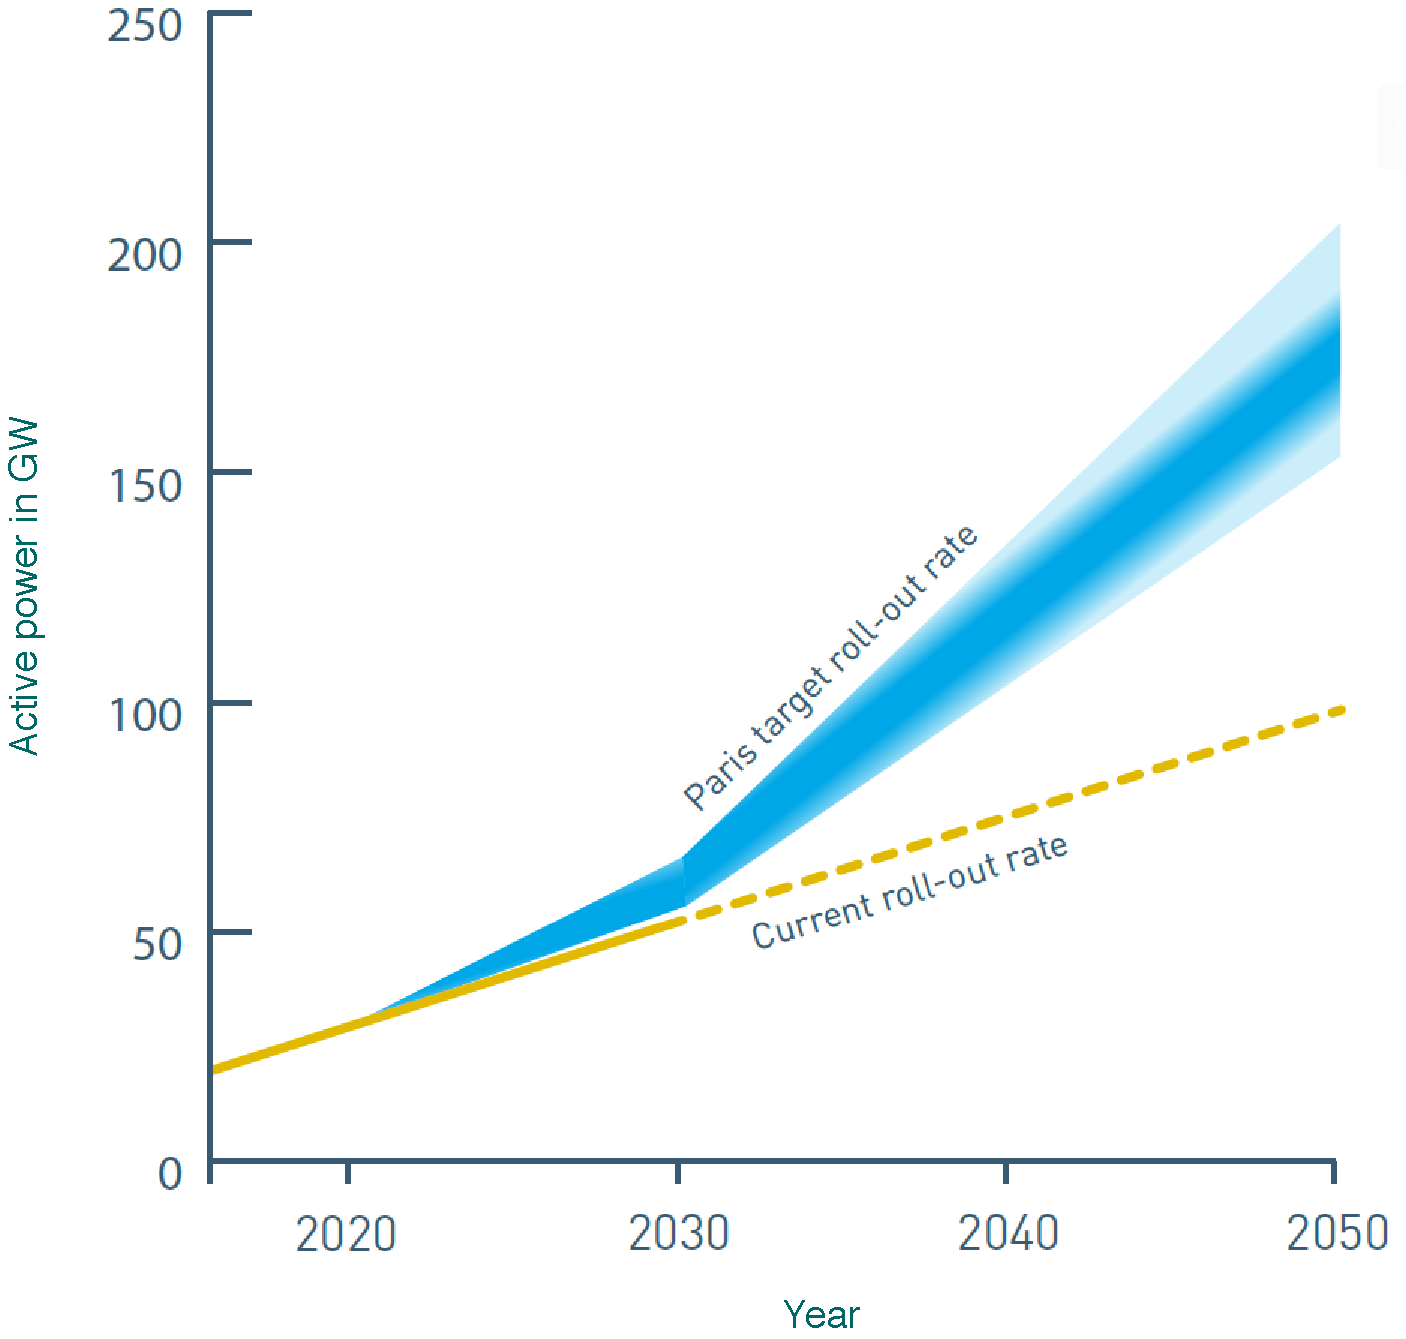
\includegraphics[height = 8.5cm,width = 9cm]{Diagrams/Chapter_1/Paris.pdf}
    \caption{Installed wind capacity in the North Sea in GW \cite{noauthor_vision_2020}}
    \label{fig:Paris_roll_out}
\end{figure}

\gls{RES} are connected to the power system through Power Electronic (\gls{PE}) converters as shown in Figure \ref{fig:Energy_conv_system_2}. The \gls{PE} converters do not possess inherent inertial response characteristics. Until now, integration of \gls{RES} to the power system has not created major problems since the stability of the system is maintained by the synchronous machines in power plants. Traditionally, the inertia for the power system is provided by these synchronous machines connected to the network (Figure \ref{fig:Energy_conv_system}). However, an increase in \gls{RES} in the future causes an increase in \gls{PE} converter based generation units. Simultaneously, the synchronous machines in the conventional power plants need to be disconnected from the network. This makes the power systems weak due to low short circuit power and low system inertia. Therefore, the consequence of disconnecting the synchronous generators leads to the requirement of the \gls{PE} converter based generation units to take up the role of governing the stability of the power system.

\begin{figure}[H]
\centering
%\hspace*{-1.2cm}
    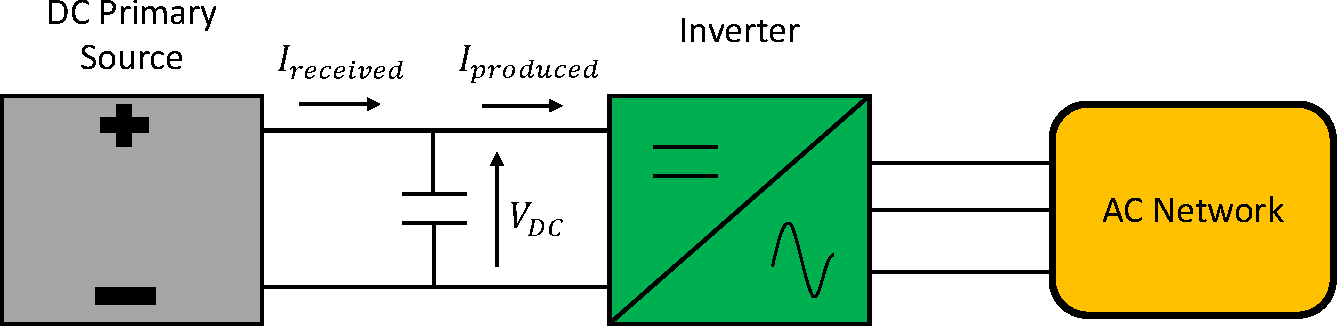
\includegraphics[height = 3cm,width = 12cm]{Diagrams/Chapter_1/Energy_conv_system_2.pdf}
    \caption{PE converter-based generation connection to the AC network \cite{denis_migrate_2018}}
    \label{fig:Energy_conv_system_2}
\end{figure}
\vspace{0mm}
\begin{figure}[H]
\centering
%\hspace*{-1.2cm}
    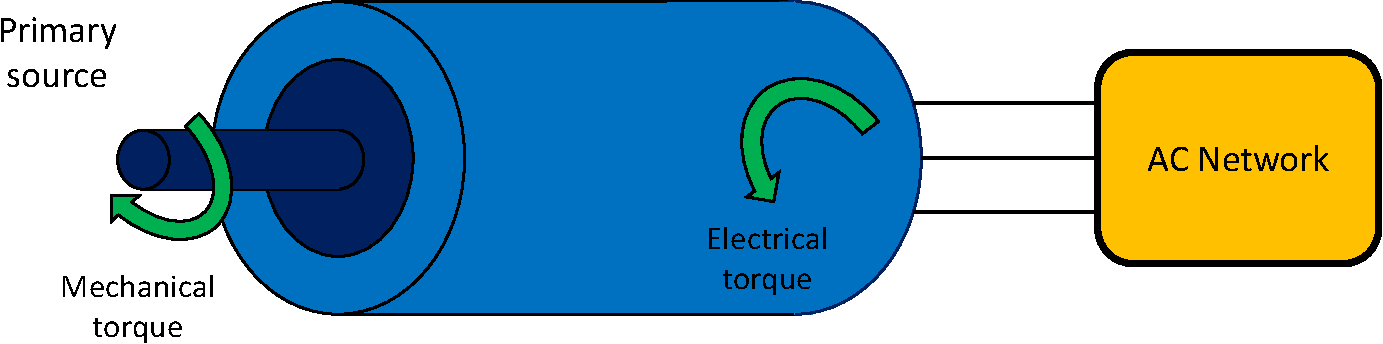
\includegraphics[height = 3cm,width = 12.5cm]{Diagrams/Chapter_1/Energy_conv_system.pdf}
    \caption{Conventional generators connection to the AC network \cite{denis_migrate_2018}}
    \label{fig:Energy_conv_system}
\end{figure}

%\section*{Small scale offshore networks}
The majorly contributing source among the available \gls{RES} is wind energy. Specifically, offshore wind energy is predicted to be the most significant source of energy among the North Sea countries by 2040 \cite{muller2017translate}. As a result, the deployment of offshore wind energy technology is expected to grow further. With the increase in integration of offshore wind energy, the inherent characteristics of offshore wind energy conversion systems will affect the nature of the power system. The vulnerable wind speed conditions due to the uncertain behaviour of wind, could lead to variations in the supply and demand and therefore, fluctuations in voltages and frequency are bound to occur. Moreover, as the power systems become weak due to the decommissioning of synchronous generators in conventional power plants that use non-renewable sources, the integration of offshore wind power plants to such weak power systems pose various research challenges on the power system stability. 


One among the challenge is related to voltage stability. The continuous variations in offshore wind speed causes constant change in the active power output of the offshore wind power plant. This could lead to an increase in the reactive power output and consequently voltage at the point of common coupling (\gls{PCC}). The conventional current control methods using Proportional Integral (\gls{PI}) controllers in the modern Wind Generators (\gls{WG}s) are capable of providing voltage control by injecting reactive currents when connected to a strong network \footnote{SCR = SC$_{MVA}$/P;\; where SC$_{MVA}$ is the short circuit power of the network and P is the active power generation. \\
If SCR = 100 to 250, it is a strong grid. If SCR = 5 to 25, it is a weak grid.}. However, these controllers are not suitable for operation in highly \gls{PE} converter dominated grids as the connected network is weak and is not capable of absorbing the injected currents. Furthermore, during the scenario of islanding, voltage control by the conventional current controllers is ineffective as the deviation in voltage is not high enough to activate a productive voltage reduction mechanism. There are challenges in terms of frequency stability  as well since the conventional current controllers in the \gls{WG}s are not equipped to provide frequency control of the network during islanding. 

Currently, the state-of-the-art technology for the transfer of offshore wind power to the onshore system is Voltage Source Converter (\gls{VSC}) based  - High Voltage Direct Current (\gls{HVDC}) transmission links. Presently, Modular Multi-level Converter (\gls{MMC}) topology that falls under the classification of \gls{VSC} topologies is the most suitable solution. Few of the advantages of \gls{MMC} are \cite{cigre_B455}, (1) ease of integration with Offshore Wind Farms (\gls{OWF})s, (2) supporting bi-directional flow of power between the offshore network and onshore system, and (3) independent control of active and reactive powers in the network. However, with the available technology, \gls{MMC}-\gls{HVDC} transmission are limited to a rated capacity of 1.2 GW \cite{peralta2012detailed}.

%\section*{Large scale offshore networks}\label{large_scale_intro}
The implementation of large scale offshore networks (greater than or equal to 2 GW) creates a highly \gls{PE} converter dominated network. The aforementioned challenges in terms of voltage and frequency control by the \gls{PE} converters without the presence of conventional units is prominent in large scale offshore networks. 

The absence of conventional generators would mean that the \gls{PE} converters will have to take into account the decreasing inertia of the system that leads to a faster dynamic behaviour and needs controllers with faster time response. Moreover, in large scale offshore networks, distant \gls{OWF}s would be connected in parallel. With parallel operation of the conventional current controllers in \gls{WG}s, interactions can persist among them and could lead to instability of the network. Additionally, the restoration of grid following disturbances by the \gls{PE} converter units is a serious matter of concern. With the conventional current control approach, grid restoration is challenging without the help of auxiliary diesel generators. However, in the case of large scale offshore networks, the role of grid restoration must be taken up by \gls{PE} converters. There can be arguments that storage facilities such as battery and thermal can be a realizable solution in case when there are no conventional generators available. Huge investment costs, low lifetime and low efficiency when compared to controller modifications are the drawbacks that make these storage facilities practically unusable in large scale offshore networks \cite{telaretti_economic_2016}.

Traditionally, the transmission of power from \gls{OWF} to the offshore converter station uses a combination of 33 kV and 145 kV \gls{HVAC} cables. The \gls{OWF}s are connected to an \gls{AC} offshore platform using 33 kV \gls{HVAC} cables. The platform holds a power transformer that is used to step-up voltage from 33 kV to 145 kV, and power is transferred from the \gls{AC} platform to the offshore converter station using 145 kV \gls{HVAC} cables \cite{abdelwahed2016power}. However, the upcoming projects are expected to have a higher voltage level of 66 kV for transmission to allow twice the amount of power transferred compared to 33 kV. Therefore, this would only require 66 kV \gls{HVAC} cables to directly connect \gls{OWF}s to offshore converter station, avoiding the use of an \gls{AC} collector platform \cite{dnv66kv}. Hence, advancing towards large scale offshore networks, it would be more appropriate to assess the performance of these networks developed with 66 kV \gls{HVAC} transmission. 

% On the \gls{OWF} side, conventionally, the \gls{OWF}s are connected to a \gls{AC} collector platform through 33 kV cables. At the platform, a 33/145 kV transformer is used to step-up the voltage and the power is transferred to the offshore converter station using 145 kV cables. However, the upcoming projects plan to have a rating of 66 kV \gls{HVAC} transmission compared to the conventional combination of 33 kV and 145 kV \gls{HVAC} transmission due to the advantages of lesser array cabling and higher power transmission. In such cases, the \gls{AC} collector platform can be avoided and power can transmitted from the \gls{OWF}s to the offshore converter station directly using 66 kV \gls{HVAC} cables \cite{dnv66kv}.

With the available \gls{MMC}-\gls{HVDC} transmission technology, multiple \gls{MMC}-\gls{HVDC} transmission links connected in parallel would be required to transfer the bulk amount of offshore wind power generated from large scale offshore networks to the onshore system. In such networks, the power flow between the parallel operated \gls{MMC}s and the \gls{OWF}s must be coordinated during steady state and dynamic conditions. The major challenges regarding voltage and frequency control during islanding of the \gls{OWF}s must be taken into account. The scenario of reactive current injection that needs to be provided by the \gls{WG}s during dynamic conditions as demanded by majority of the grid codes must also be taken into consideration \cite{mohseni_review_2012}. Therefore, the progress towards the development of large scale offshore networks calls for a generic model with a suitable layout with the available technology that is capable of tackling the aforementioned technical challenges and providing stable operation during steady state and dynamic conditions. 
% the connection of distant \gls{OWF}s also creates challenges for the system operators. High Voltage Direct Current (\gls{HVDC}) transmission is preferred over High Voltage Alternating Current (\gls{HVAC}) for longer distances due to lower losses and lower investment costs \cite{ryndzionek_evolution_2020}. Conventionally, 


\section{Literature Review}\label{lit_review}

As seen in Section \ref{Background}, the major challenges are; development of large scale offshore networks with available technology is challenging, no much knowledge about 66 kV \gls{HVAC} transmission available, and new control strategies are required that can provide better control of voltage and frequency. Hence, a generic model for large scale offshore networks with the latest trend in available technology, and enhanced control strategies is a key research requirement. 
% The literature review is mainly focused on three aspects: 1) control strategies to overcome the technical challenges related to voltage and frequency control in \gls{WG}s, 2) power transfer from the \gls{OWF}s to the offshore \gls{MMC} converter and 3) topology of  
% Going with the latest trend, different approaches are available for connection of \gls{MMC}s.

Based on \gls{MMC}-\gls{HVDC} transmission technology, there are mainly three configurations available for the connection of offshore and onshore converter stations \cite{cigre_B455}, \cite{sharifabadi2016design}: 
\begin{itemize}
    \item Point-to-point connection: The configuration connects one \gls{OWF} to the offshore converter station, which is then connected using \gls{HVDC} link to the onshore converter station.
    \item Multi-infeed connection: The configuration involves connecting one \gls{OWF} to two different onshore systems by connecting two offshore converter stations on a common bus on the Alternating Current (\gls{AC}) side and transmitting power through two \gls{HVDC} links. Such a configuration allows for increasing the rating of the \gls{OWF} beyond the capacity of a single offshore converter station. The drawback of such a configuration is that, it allows the connection of only one \gls{OWF} to the network.
    \item Multi-Terminal Direct
    Current (MTDC) connection: In this configuration, the \gls{HVDC} links of multiple offshore converter stations are connected to a main Direct Current (\gls{DC}) link. Such a configuration enables transfer of active power to the onshore system depending on the capacity of the main \gls{DC} link. The drawback of such a configuration is that, a complete shut down and restart of the connected \gls{MMC}s is required for a fault on the \gls{DC} side.
\end{itemize}

The multi-infeed and the MTDC connections allow for parallel operation of \gls{MMC}s which is a significant requirement for large scale offshore networks with the available technology. But both the configurations have the drawback of being able to connect only one \gls{OWF} to the network. Therefore, configurations that utilize several \gls{OWF}s with parallel operation of \gls{MMC}s are currently unavailable and is a key area of research. The topology mentioned in \cite{lozada_ayala_dynamic_2018} embraces the utilization of 66 kV \gls{HVAC} transmission from the \gls{OWF}s (all connected in parallel) to the offshore converter station. However, the topology examined does not utilize parallel operation of \gls{MMC}s and uses only one \gls{MMC}-\gls{HVDC} link with a maximum power transfer capacity of 1 GW.

% On the \gls{OWF} side, 

%The technical challenges regarding voltage and frequency control are key aspects to be considered for the development of large scale networks.
Typically, \gls{PE} converters in the \gls{WG}s are connected to the network for parallel operation using present state-of-the-art technology, current control strategies. In such control strategies, the regulation of power output of the converters is achieved by measuring the angle of the grid voltage. The drawback of these control strategies is that they require an already existing reference voltage. There are control strategies that create the reference voltage and are termed as voltage control strategies. One among the voltage control strategies is the V/F (voltage/frequency) control that is utilized for operation in the islanded mode. The drawback with V/F control is that it is not equipped for the parallel operation of various voltage forming converter units \cite{weise2019comparison}. Therefore, there needs to be new control strategies in the \gls{WG}s that can create the reference voltage and work in parallel operation. Such control strategies are an emerging area of research. There are studies performed to implement control strategies that can create voltage reference and work in parallel operation as well. Few among them are mentioned as follows:

% European Network of Transmission System Operators for Electricity (ENTSO-E) classifies converters into three classes (Class 1, Class 2 and Class 3) and the converters working with the strategies mentioned above are categorized under Class 3. The complete requirements that need to be complied by such converters are depicted in \cite{christensen2020high}.

\begin{itemize}
    \item Virtual Synchronous Machines (VSM): The \gls{PE} converter control is modelled with the characteristics of a synchronous machine in terms of inertia and voltage support by correspondingly deriving the equations \cite{markovic2018lqr}, \cite{duckwitz_operating_behavior}, \cite{lu_virtual_2019}.
    
    \item Modified Droop Control:
    This strategy is common for standalone grids, where the parallel operation of voltage forming units is developed recently using the f/P (frequency/active power) and V/Q (voltage/reactive power) droop controls similar to the control in synchronous generators \cite{bouzid2016simulation}. Few authors have named these droop control concepts as Virtual Synchronous Machines Without Inertia (VSCM0H) \cite{yu2016use}.
    
    \item Direct Voltage Control (\gls{DVC}):
    \gls{DVC} is a representation of the conventional current control approach towards a voltage control. \gls{DVC} allows for the direct control of the \gls{AC} converter voltage which in turn varies the current injected by the converter  \cite{korai_dynamic_2019}, \cite{erlich_new_2017}. This approach provides continuous voltage control both in steady-state and dynamic scenarios. %This control method is implemented for analysis in this thesis work.
    
    \item Extended Current Control:
    The control is similar to the conventional current control with an additional inertia control in the outer control loop by using a synthetic inertia controller that gives a behaviour similar to that of a synchronous machine \cite{duckwitz_derivation_2019} \cite{liu2017control}. 
\end{itemize}

Studies performed by I. Erlich et al. and A. Korai et al. in \cite{erlich_new_2017} and \cite{korai_dynamic_2019} show appealing results of the implemented \gls{DVC} for highly \gls{PE} dominated systems. The simulations are tested for different grids based on real world data and provide promising outcomes with effective voltage and frequency control. Hence, with such proven results and available models, the \gls{DVC} strategy was chosen to be incorporated for this work. Moreover, the real-time implementation of \gls{DVC} in Type-4 \gls{WG} is attempted in \cite{sethi_real-time_nodate-new}, but the latest trend of 66 kV \gls{HVAC} transmission and the major requirement of reactive current injection by the \gls{WG}s during dynamic conditions is lacking.

It is also good to analyze the effectiveness of other control strategies mentioned above. With a generic offshore network model, different control strategies can be implemented in the \gls{OWF}s and the complexity related to the interoperability of the controllers can be assessed. However, this lies beyond the scope of this project.

\section{Objectives and Research Questions}
The overall goal of the thesis is to develop a generic digital twin model of 2 GW, 66 kV \gls{HVAC} offshore network and to perform analysis on the dynamics of voltage and power at various locations in the network. The thesis makes use of the Electro-Magnetic Transient (\gls{EMT}) simulation-based software tools such as RSCAD and PowerFactory to analyze the performance of the developed control models. The average model of Type-4 \gls{WG} available in RSCAD is used as a starting point. The thesis provides a detailed description of the different available features in RSCAD that are employed to develop the 2 GW model. 
To achieve the overall goal, the following research questions are defined:
\begin{itemize}
    \item How effective is the Direct Voltage Control (\gls{DVC}) when implemented in an \gls{EMT} average model of Type-4 \gls{WG} connected to a 66 kV equivalent \gls{HVAC} system in RSCAD?
    
    \item What insights can be attained by the \gls{EMT} average model of Type-4 \gls{WG} with \gls{DVC} in 66 kV network in RSCAD in comparison with a similar network modelled with a simplified Type-4 \gls{WG} configuration with \gls{DVC} in DIgSILENT PowerFactory?
    
    \item How can Type-4 \gls{WG}s with implemented \gls{DVC} work in coordination with offshore \gls{MMC}s within a multi-gigawatt offshore transmission network?
    
    \item How effectively do Type-4 \gls{WG}s with implemented \gls{DVC} perform when connected in an offshore network for parallel operation?

\end{itemize}

\section{Thesis Contribution}
On behalf of the thesis objectives defined above, the key contributions from this thesis are presented in this section.

\begin{itemize}
    \item Implementation of the \gls{DVC} in Type-4 \gls{WG} model in RSCAD for an offshore 66 kV \gls{HVAC} network. With proper documentation provided in this report, the developed 66 kV \gls{HVAC} model in RSCAD can be utilized for future work.
    
    \item Development of a 66 kV \gls{HVAC} offshore network in PowerFactory by adapting the benchmark \gls{DVC} model in Type-4 \gls{WG}s. With proper documentation provided in this report, the developed 66 kV \gls{HVAC} model in PowerFactory model can be utilized for future work.
    
    \item Development of a digital twin of 2 GW, 66 kV \gls{HVAC} offshore network with \gls{DVC} implemented in Type-4 \gls{WG}s connected to two offshore converter stations in RSCAD. With proper documentation provided in this report, the developed 2 GW model in RSCAD can be utilized for future work.
    
    \item Automation script for the operation of the developed 2 GW offshore network model using the interface between RSCAD and MATLAB is created. %With proper documentation provided in this report, the script can be utilized for future work.
\end{itemize}

\section{Thesis Outline}
A brief outline of the methodology is structured in several chapters, which sequentially describe the performed tasks as follows:
\begin{itemize}
    \item Chapter \ref{2}: The chapter presents the concepts of wind energy conversion system and the classification of wind turbines. The overview of the \gls{OWF} network with all the major equipment and the latest trend in technology is explained. The issues with the present current control strategies and the necessity to move towards better control strategies are addressed. The new control strategy, \gls{DVC}, to be implemented in Type-4 \gls{WG} is formulated.  
    
    \item Chapter \ref{3}: The implementation of \gls{DVC} in \cite{korai_dynamic_2019} and \cite{sethi_real-time_nodate-new} for a digital twin of 66 kV \gls{HVAC} offshore network in RSCAD is detailed. The performance of Type-4 \gls{WG} with \gls{DVC}, in terms of short-term voltage stability and reactive current injection, under severe disturbances is analyzed. Modelling of a similar 66 kV \gls{HVAC} offshore network in DIgSILENT PowerFactory tool is also addressed. The comparison of the dynamic performance of \gls{DVC} in two \gls{EMT} platforms (RSCAD and PowerFactory) for a 66 kV \gls{HVAC} offshore network during severe disturbances is carried out. 
    
    \item Chapter \ref{4}: The development of a large scale digital twin model of a 2 GW offshore network in RSCAD is detailed. The modifications in the control structures of the \gls{MMC}s to work in coordination with the implemented \gls{DVC} in \gls{WG}s are addressed.
    
    \item Chapter \ref{5}: The operation of the developed large scale 2 GW network is discussed. The interplay of offshore \gls{MMC}s and Type-4 \gls{WG}s in terms of dynamic power flow control within the offshore network (by analyzing the voltage and current profiles in the electrical path between the \gls{WG}s and the \gls{MMC}s) is performed. 
    
    \item Chapter \ref{6}: The significant conclusions for the research questions are provided. The future scope and recommendations are also added.
\end{itemize}

A figurative representation of the thesis workflow is presented in Figure \ref{fig:Thesis_outline}.

\begin{figure}[H]
\centering
%\hspace*{-1.2cm}
    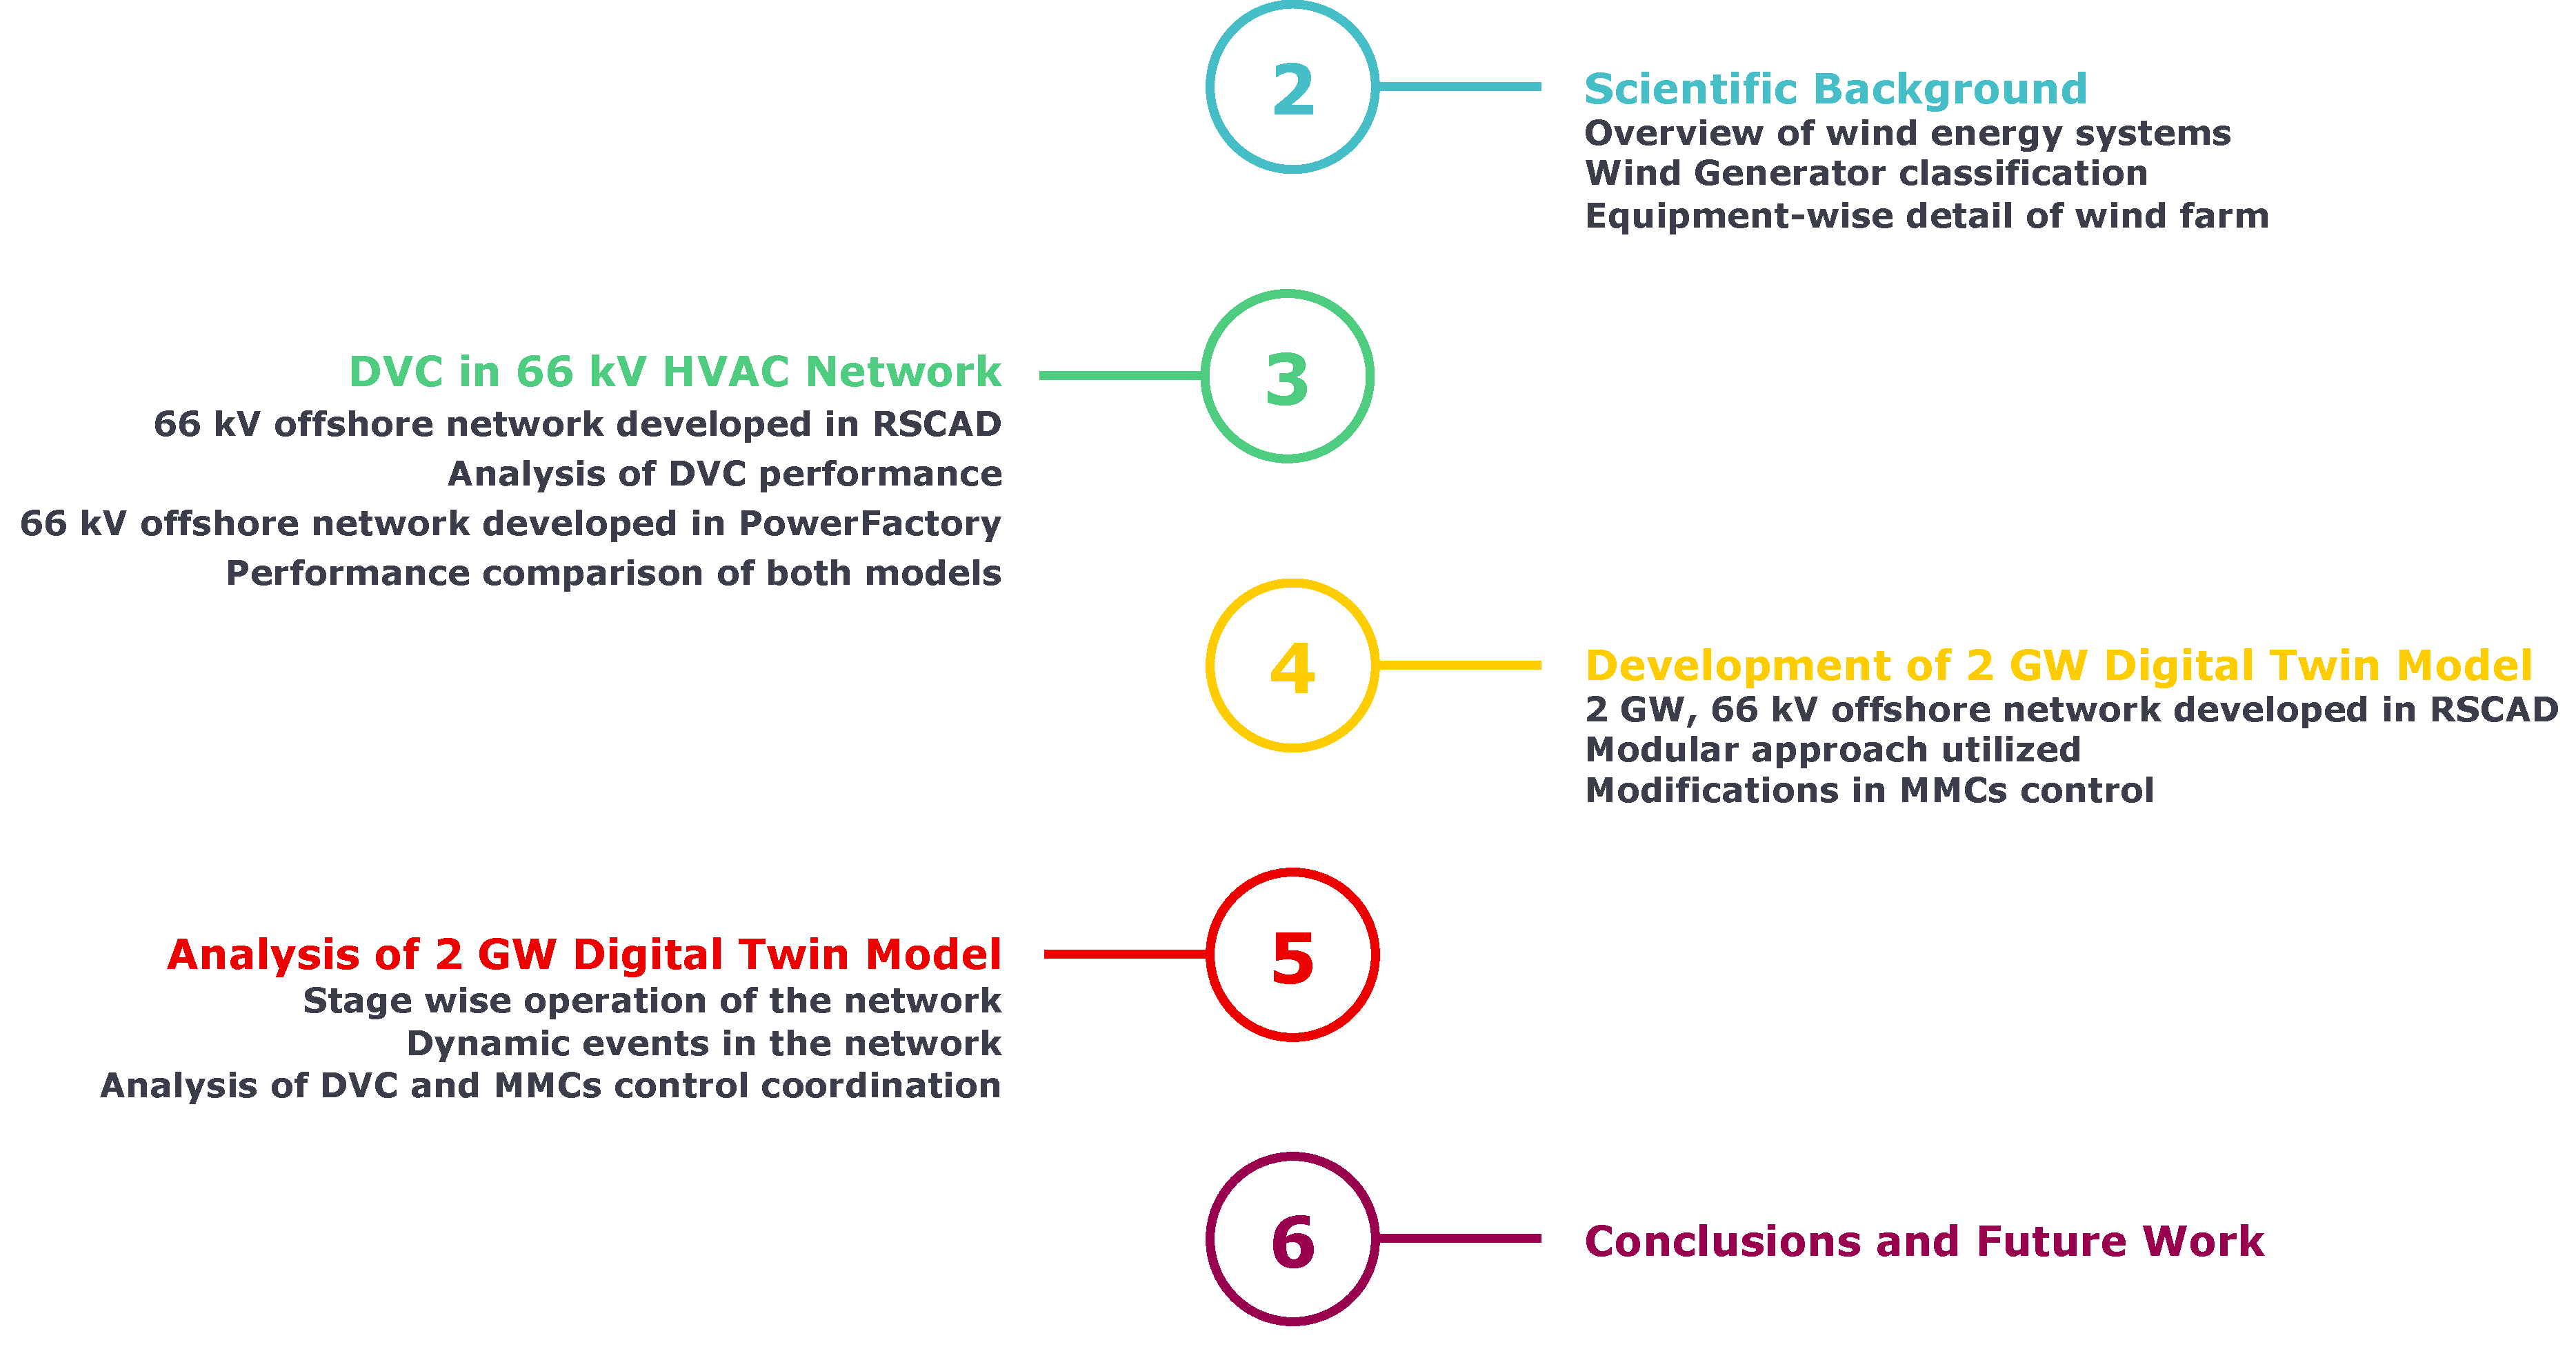
\includegraphics[height = 9.5cm,width =\textwidth]{Diagrams/Chapter_1/Thesis_flowchart.pdf}
    \caption{Work flow of thesis}
    \label{fig:Thesis_outline}
\end{figure}

% \chapter{Scientific Background}\label{2}
An outline of the fundamentals required for this thesis work is presented in this chapter. Firstly, the basics of wind energy conversion systems are explained. All components that are a part of an offshore wind farm network are depicted and explained. The conventional control topologies in \gls{VSC}s are also explained.

\section{Wind Energy Conversion Systems (WECS)}\label{WECS_theory}
The \gls{WECS} is a mixture of various engineering fields such as mechanical, electrical and control systems. The \gls{WECS} consists of several components that convert the kinetic energy of the wind into electrical energy and transfer power efficiently and systematically. The major mechanical equipment in the \gls{WECS} are the turbine tower, nacelle, rotor blades, hub, drives, gearbox, drive-train and mechanical brakes \cite{manwell2010wind}. The power \gls{PE} converters, electrical generator, transmission cables, power transformers and transmission towers constitute the electrical part. The control systems \cite{yaramasu_high-power_2015} governs both the electrical and mechanical systems.
The basic structure of the wind energy conversion system is depicted in Figure \ref{fig:WECS}.   

\begin{figure}[H]
\centering
%\hspace*{-1.2cm}
    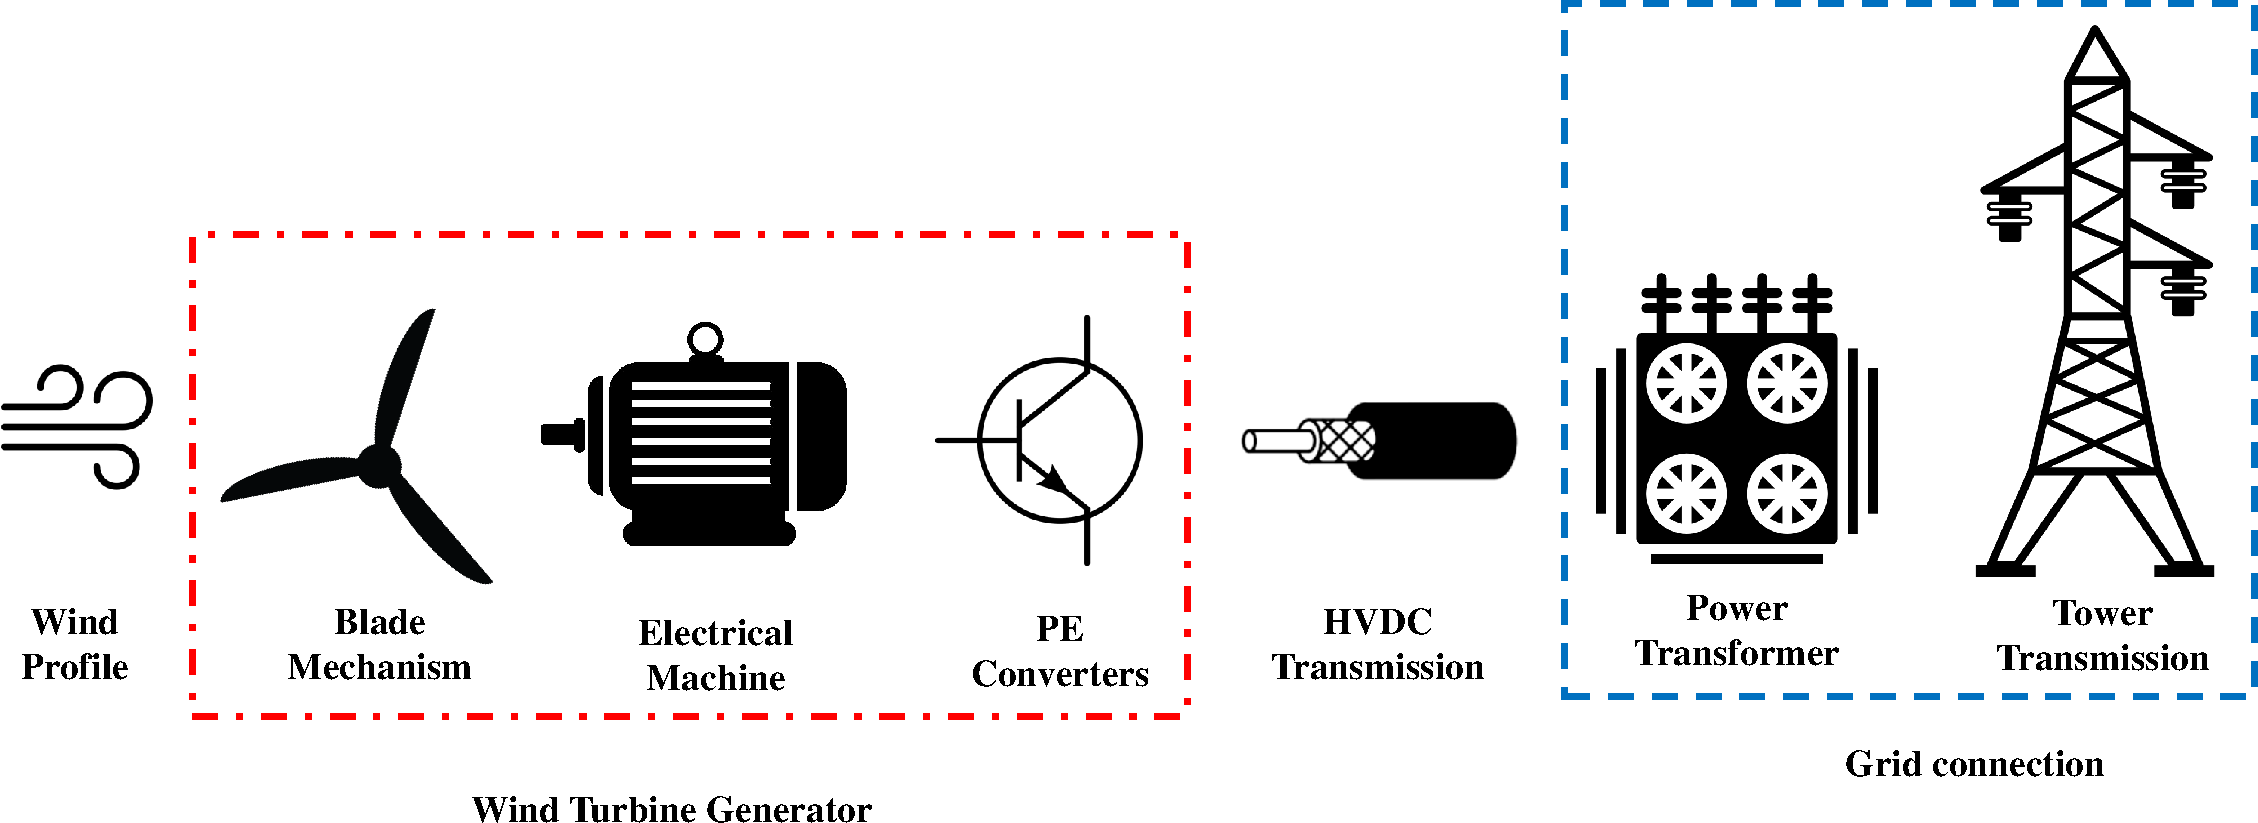
\includegraphics[height = 5.5cm,width = 15.5cm]{Diagrams/Chapter_2/WECS.pdf}
    \caption{Schematic of offshore wind power transmission}
    \label{fig:WECS}
\end{figure}

\section{Power from Wind Energy} 
The wind energy converts kinetic energy of the wind to mechanical energy or electrical energy. Wind energy is represented as the kinetic energy of moving air mass. The mechanical power extracted from practical wind turbines can be depicted as in Equation \ref{windenergy} \cite{ali_wind_2012}.

\begin{equation}\label{windenergy}
    P_m =\frac{1}{2} C_p(\lambda,\beta) \rho A v_m^3 = C_p P_w
\end{equation}

where $C_p$ is the power coefficient, $P_m$ is the power from wind and $v_m$ being wind speed. $\lambda$ is the tip speed ratio, and $\beta$ is the blade pitch angle in degrees. 

The tip speed ratio, $\lambda$ is defined as,
\begin{equation}
\lambda= \frac{R\omega}{v} 
\end{equation}
where R is the turbine blade radius in meters and $\omega$ is the mechanical angular velocity in rad/s and $v$ is the wind speed in m/s.    

The coefficient of performance, $C_p$, is not a constant value and is a function of $\lambda$ and $\beta$.

The $C_p$-$\lambda$ characteristics are represented for different pitch angle ($\beta$) values in Figure \ref{fig:pitchangle}. As can be seen, there exists a maximum mechanical power that can be achieved for a specific speed ratio and pitch angle.

\begin{figure}[H]
\centering
%\hspace*{-1.2cm}
    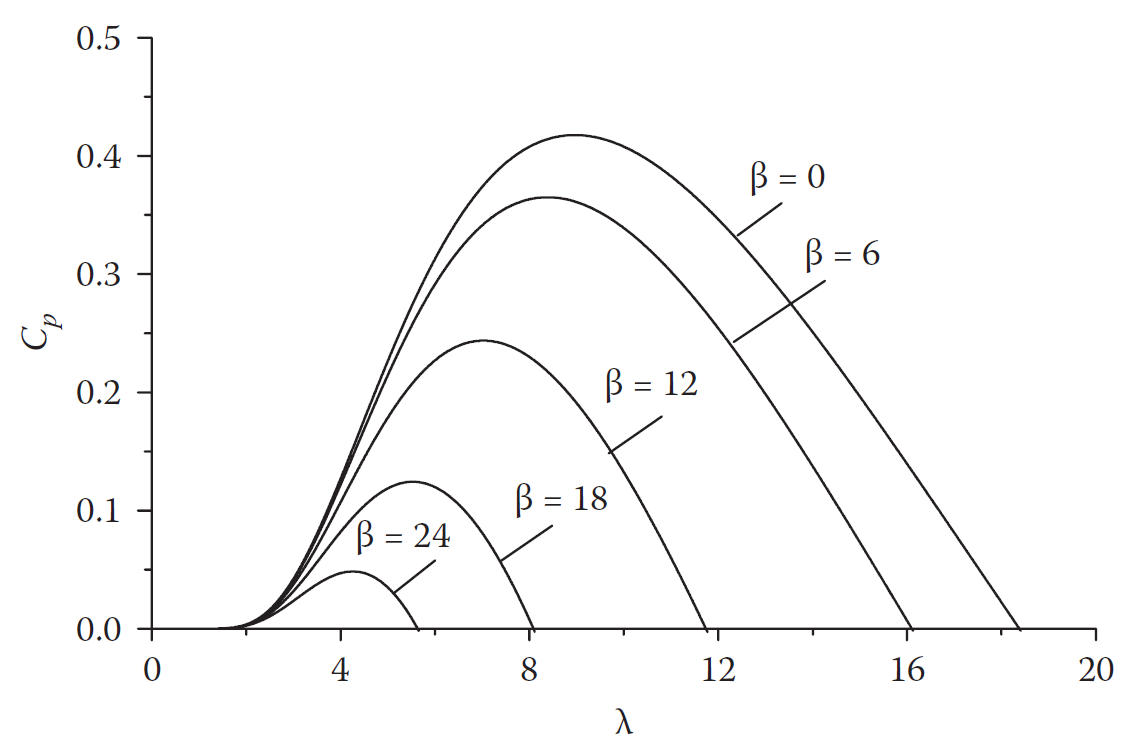
\includegraphics[height = 7.5cm,width = 11.5cm]{Diagrams/Chapter_2/pitchangle_1.png}
    \caption{Characteristics of $C_p$-$\lambda$ for various pitch angle \cite{ali_wind_2012}}
    \label{fig:pitchangle}
\end{figure}

\section{Wind Turbine Generator}
The Wind Turbine Generator (also termed as Wind Generator (\gls{WG}) ) consists of the mechanical equipment mentioned in Section \ref{WECS_theory}, the electrical generator and the \gls{PE} converters as shown in Figure \ref{fig:WECS}. Depending on the speed of operation, \gls{WG}s can be classified as follows \cite{ali_wind_2012}:

\begin{itemize}
    \item \textbf{Type 1 - Fixed speed Induction Generator (FSIG) :} Type 1 \gls{WG} has a fixed speed of operation. Hence, maximum power extraction at all times is not possible.
    \item \textbf{Type 2 - Slip Ring Induction Generator (SRIG) :} Type 2 \gls{WG} is a variable speed technology that uses a variable resistor in the rotor windings to adjust the rotor speed. However, the variation of speed is limited in this technology, and higher heat dissipation exists due to the variable resistance.
    \item \textbf{Type 3 - Doubly-Fed Induction Generator (DFIG) :} Type 3 \gls{WG} also comes under the variable speed technology. The configuration is depicted in Figure \ref{fig:Type3}. The grid transformer is directly connected to the stator of the DFIG, and the rotor is connected through a partially rated \gls{PE} converter. This configuration adds variable frequency \gls{AC} excitation (instead of only resistance) to the rotor circuit. The additional excitation for the rotor is provided through slip rings by the Voltage Source Converter (\gls{VSC}) which controls rotor currents and thereby controls the torque and reactive power of the generator. This \gls{VSC} is the Machine Side Converter (\gls{MSC}) and is connected back-to-back with a Grid Side Converter (\gls{GSC}), which provides control of the \gls{DC} link voltage and the reactive power flow to the grid. The downside of this topology is that it requires gearbox for operation and hence the chances of wear and tear is high.
    
    \begin{figure}[H]
\centering
%\hspace*{-1.2cm}
    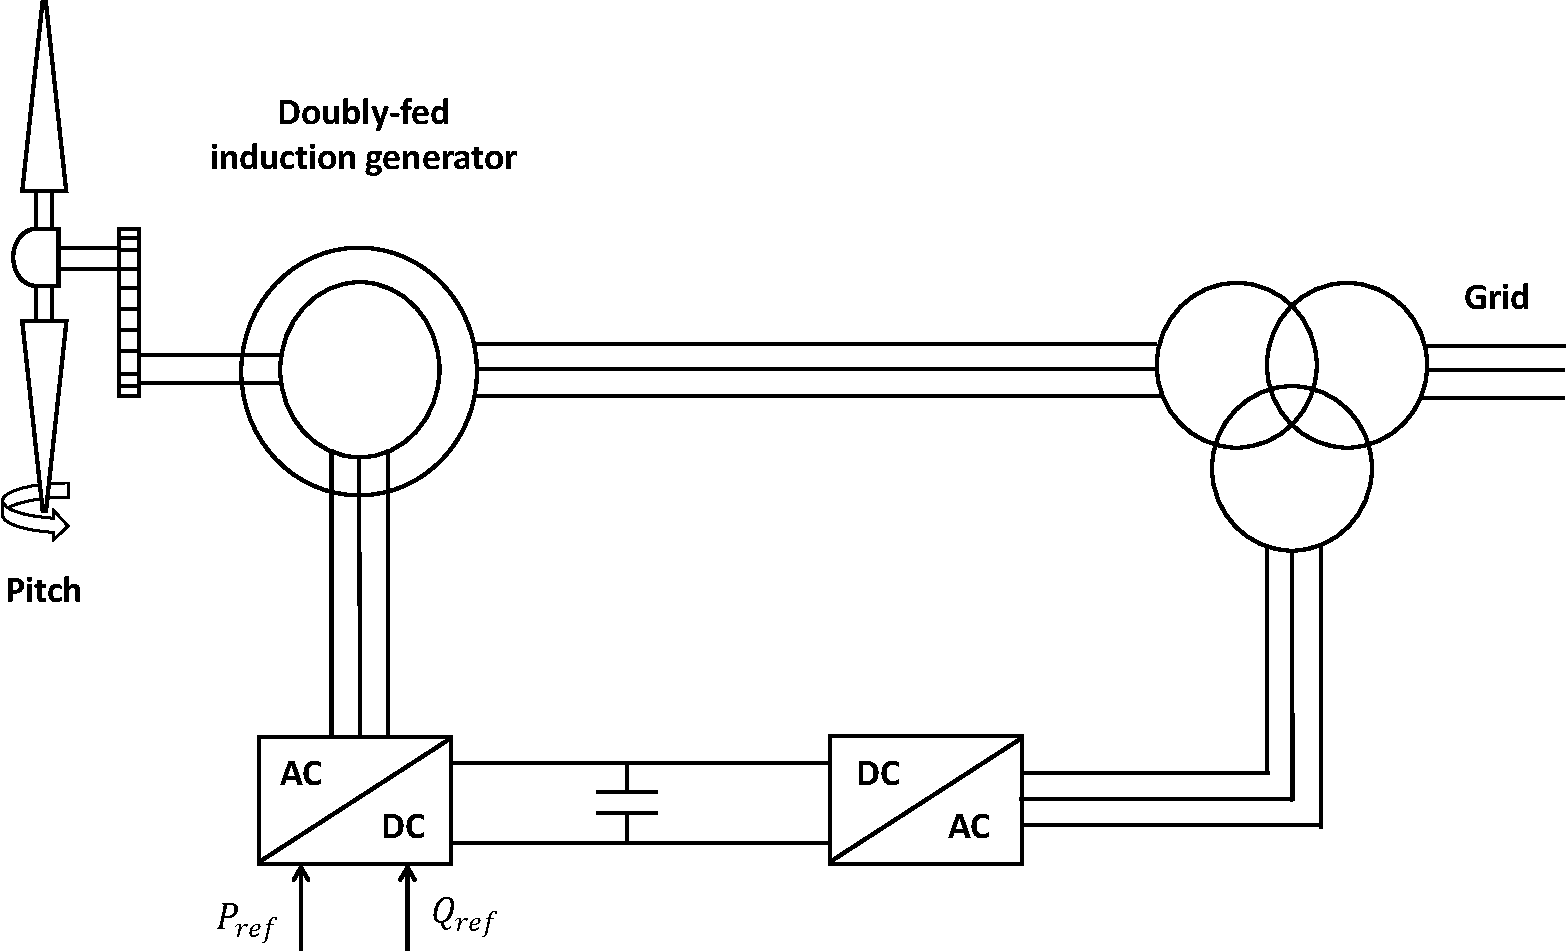
\includegraphics[height = 6.5cm,width = 12cm]{Diagrams/Chapter_2/Type3WT_new.pdf}
    \caption{Type 3 WT configuration \cite{ali_wind_2012}}
    \label{fig:Type3}
\end{figure}
    
    \item \textbf{Type 4 - Permanent Magnet Synchronous Generator (PMSG) :} Type-4 \gls{WG} also has a variable speed configuration as shown in Figure \ref{fig:Type4}. \gls{PMSG} is connected to the grid transformer through a full-scale back-to-back power converter. There is no speed limit in this topology when compared to Type-3 configuration. Another advantage in Type-4 \gls{WG} is that the gearbox can be avoided. The control structures of the converters are explained in the following sections.
    
\begin{figure}[H]
\centering
%\hspace*{-1.2cm}
    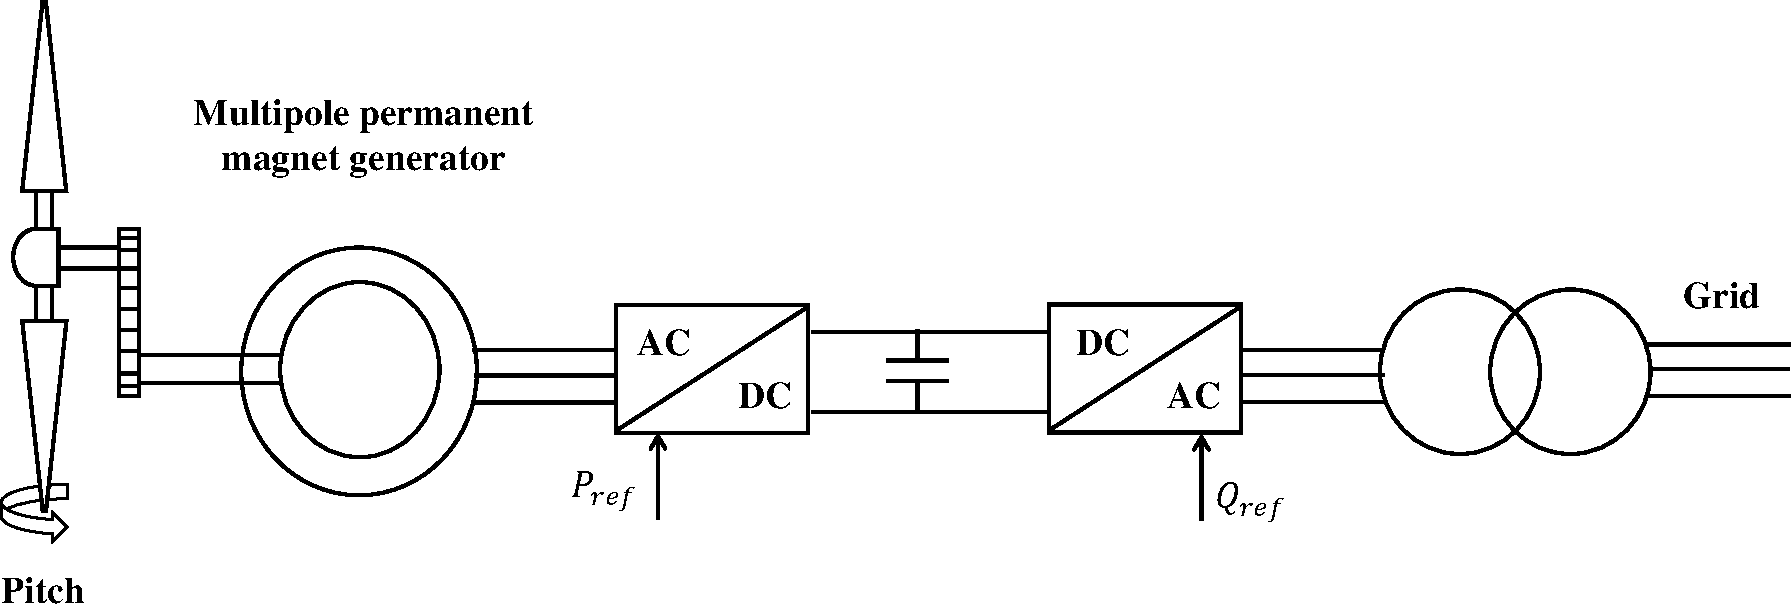
\includegraphics[height = 4.5cm,width = 13cm]{Diagrams/Chapter_2/Type4WT_new.pdf}
    \caption{Type-4 WT configuration \cite{ali_wind_2012}}
    \label{fig:Type4}
\end{figure}
\end{itemize}

Type-4 \gls{WG}s are employed for this thesis work, and hence the components involved for this architecture are explained further.

\subsection{Permanent Magnet Synchronous Generator (PMSG)}\label{PMSG}
As shown in Figure \ref{fig:PMSG}, \gls{PMSG} consists of stator, rotor and windings. The rotor is generally a permanent magnet that creates the magnetic flux. The stator consists of windings that are sinusoidally distributed. Generally, wound-field synchronous generators require \gls{DC} excitation to be provided by an external source. Whereas in \gls{PMSG}, external \gls{DC} excitation is not required, as it is created using the permanent magnets present in the rotor. Based on the direction of flux lines, \gls{PMSG} can be classified as radial flux, axial flux and transverse flux. Another classification is based on the location of permanent magnets on the rotor as inset \gls{PMSG}s and surface mounted \gls{PMSG}s \cite{sebastian_transient_1989}.  

\begin{figure}[]
\centering
%\hspace*{-1.2cm}
    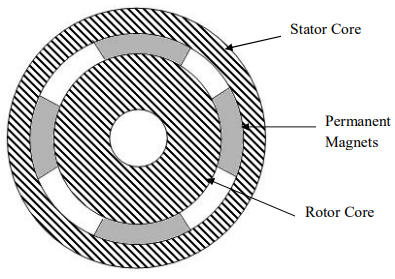
\includegraphics[height = 4.5cm,width = 6.5cm]{Diagrams/Chapter_2/PMSG.PNG}
    \caption{Cross section of a PMSG \cite{sebastian_transient_1989}}
    \label{fig:PMSG}
\end{figure}

The mathematical model of \gls{PMSG} is based on Direct-Quadrature (\gls{dq}) theory. The differential equations for the \gls{PMSG} in \gls{dq} frame are depicted in Equation \ref{PMSG_Timeeq} \cite{sebastian_transient_1989}.  

\begin{equation}\label{PMSG_Timeeq}
\begin{aligned}
    v_d = r_s . i_d + \frac{d}{dt} \Psi_d +\omega_r . \Psi_q \\
    v_q = r_s . i_q + \frac{d}{dt} \Psi_q +\omega_r . \Psi_d
\end{aligned}
\end{equation}

where $i_d$ and $i_q$ are the stator d and q axes currents respectively, $v_d$ and $v_q$ are the stator d and q axes voltages respectively. $r_s$ is the stator resistance and $\omega_r$ is electrical speed in rad/s. $\Psi_d$ and $\Psi_q$ are the d and q axes flux linkages respectively.

The flux linkages $\Psi_d$ and $\Psi_q$ are given by the Equation \ref{PMSG_psieq} \cite{rtds_tech}.

\begin{equation}\label{PMSG_psieq}
\begin{aligned}
    \Psi_d = L_d . i_d + L_{md} . i_D  + \Psi_m \\
    \Psi_q = L_q . i_q + L_{mq} . i_Q
\end{aligned}
\end{equation}

where $L_d$ and $L_q$ are the inductances in d and q axes respectively and $\Psi_m$ is the permanent magnet flux linkage.

The equivalent circuit in \gls{dq} frame is shown in Figure \ref{fig:PMSG_equiv_ckt}. The effects of permanent magnets are represented by a current source in the d-axis circuit. Equation \ref{Currentsource_MagFluxeq} shows the correspondence between the current source and the permanent magnet flux linkage.

\begin{equation}\label{Currentsource_MagFluxeq}
    \Psi_m = L_{md} . i_m
\end{equation}

\begin{figure}[H]
\centering
%\hspace*{-1.2cm}
    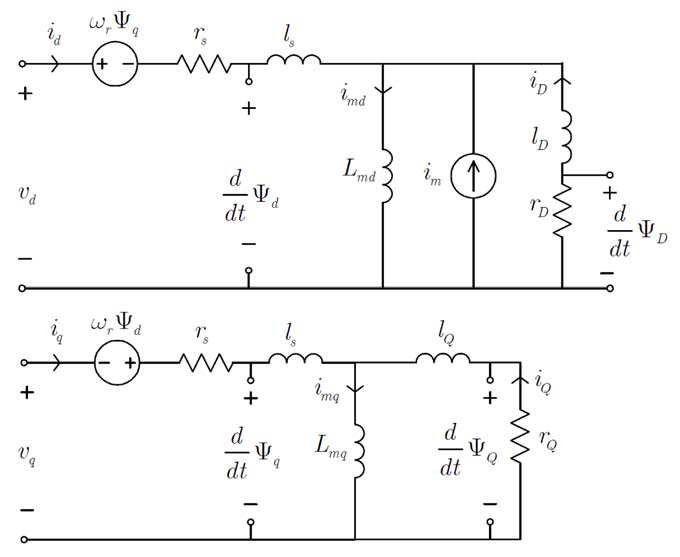
\includegraphics[height = 6.5cm,width = 8.5cm]{Diagrams/Chapter_2/PMSG_equiv_ckt.png}
    \caption{d and q axes equivalent circuit of PMSG \cite{sebastian_transient_1989}}
    \label{fig:PMSG_equiv_ckt}
\end{figure}

\subsection{Voltage Source Converter (VSC)}\label{VSC_theory}
The stator of the \gls{PMSG} is connected directly to the \gls{AC} side of a \gls{VSC} as seen in Figure \ref{fig:Type4}. This \gls{VSC} which works as a rectifier during generation operation, is termed as \gls{MSC}. It is interfaced back to back with another \gls{VSC} that works as an inverter during generation operation and is called \gls{GSC}.

\gls{VSC} consists of self-commutated switching devices such as the Insulated Gate Bipolar Transistors (\gls{IGBT}s) and anti-parallel diodes. and hence allows bidirectional flow of power between the \gls{AC} and \gls{DC} sides. The output voltage is obtained by switching off the \gls{IGBT}s. The \gls{VSC}s are classified as two-level or multi-level depending on the number of voltage levels they can generate \cite{noauthor_appendix_2014-1}. 

\subsubsection{Two-level VSC}
The two-level \gls{VSC} is the most commonly used type of converter in various applications because of the simplicity of its operation. The configuration of a two-level \gls{VSC} is depicted in Figure \ref{fig:2levelVSC}. Voltages of (1/2 $V_{dc}$, -1/2 $V_{dc}$) can be obtained in two-level \gls{VSC} as shown in the graph in Figure \ref{fig:2levelVSC}. The operation of switches $S_{1}$ and $S_{2}$ in two-level \gls{VSC} are complementary to prevent short circuit across the \gls{DC} link and hence protecting the power electronic devices from being subjected to over-current.

\begin{figure}[H]
\centering
%\hspace*{-1.2cm}
    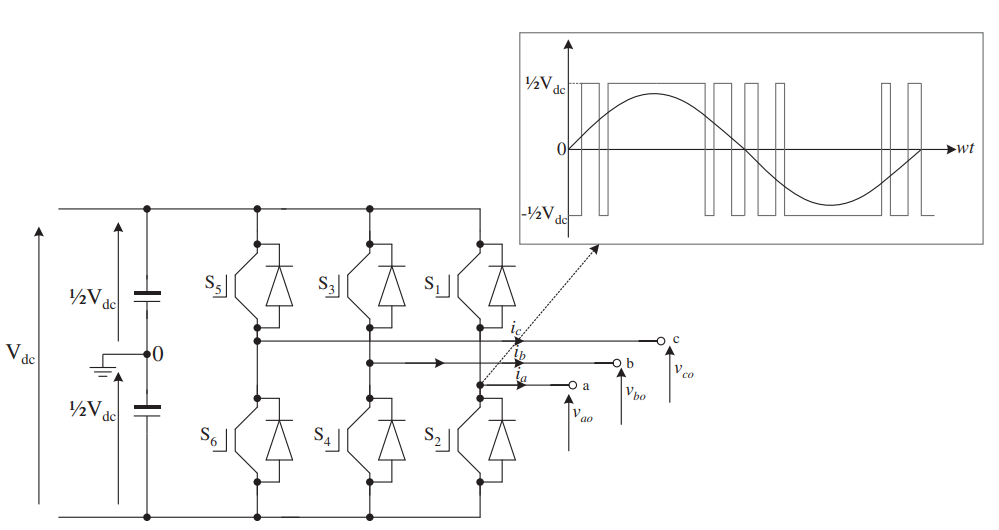
\includegraphics[height = 7.5cm,width = 15.5cm]{Diagrams/Chapter_2/2levelVSC.PNG}
    \caption{Two-level VSC \cite{noauthor_appendix_2014-1}}
    \label{fig:2levelVSC}
\end{figure}

\subsubsection{Multi-level VSC}
\gls{VSC}s with three or more levels are termed as multi-level \gls{VSC}s. The three-level \gls{VSC} is among the first multi-level configuration used on large scale and is also termed as Neutral Point Clamped (\gls{NPC}) converter \cite{sharifabadi2016design}. The topology of a \gls{NPC} converter is shown in Figure \ref{fig:3levelVSC}. The voltage levels of (1/2 $V_{dc}$ , 0 , -1/2 $V_{dc}$) can be obtained for a \gls{NPC} converter. This provides a better sinusoidal nature and also reduces the Total Harmonic Distortion (THD) when compared to a two-level \gls{VSC}. The switches ($S_{a1}$,$S_{a3}$) and ($S_{a2}$,$S_{a4}$) are complementary in the \gls{NPC} converter. This means, turning on switch $S_{a1}$ eliminates $S_{a3}$ from being turned on and the same pattern is followed for the latter complementary pair. The summary of switching operation for a \gls{NPC} converter is shown in Table. \ref{tab:3level_switching}. 

\begin{figure}[H]
\centering
%\hspace*{-1.2cm}
    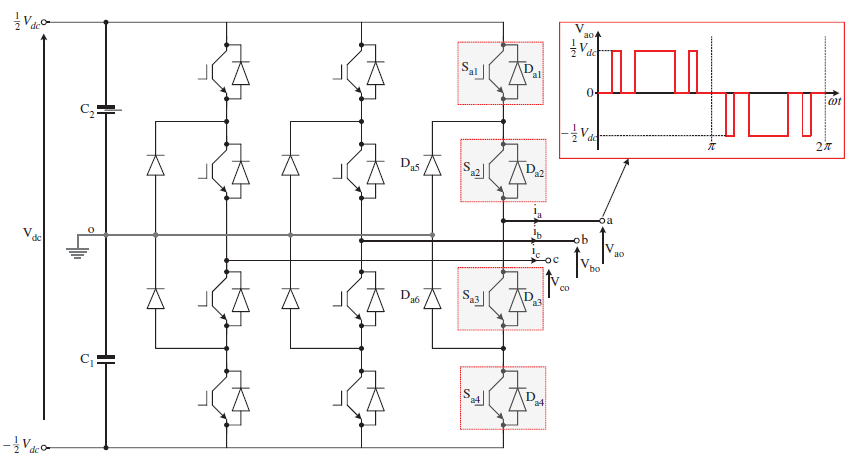
\includegraphics[height = 6.5cm,width = 14.5cm]{Diagrams/Chapter_2/3levelVSC.PNG}
    \caption{Three-level VSC or NPC Converter \cite{noauthor_appendix_2014-1}}
    \label{fig:3levelVSC}
\end{figure}

\begin{table}[H]
\centering
\begin{tabular}{c|c|c|c|c|}
\cline{2-5}
                                          & \multicolumn{4}{c|}{Switch state}     \\ \hline
\multicolumn{1}{|c|}{Voltage level}       & $S_{a1}$ & $S_{a2}$ & $S_{a3}$ & $S_{a4}$ \\ \hline
\multicolumn{1}{|c|}{$\frac{1}{2}V_{dc}$}  & ON      & ON      & OFF     & OFF     \\ \hline
\multicolumn{1}{|c|}{0}                   & OFF     & ON      & ON      & OFF     \\ \hline
\multicolumn{1}{|c|}{$-\frac{1}{2}V_{dc}$} & OFF     & OFF     & ON      & ON      \\ \hline
\end{tabular}
\caption{Switching operation of a three-level VSC \cite{noauthor_appendix_2014-1}}
\label{tab:3level_switching}
\end{table}

\subsubsection{Pulse Width Modulation (PWM)}
The switching of the valves has to be configured using a control mechanism to ensure proper operation. To reduce the harmonic content and to control the magnitude of output voltage, many Pulse Width Modulation (\gls{PWM}) techniques are developed. Few of them used currently are, Selective Harmonic Elimination (SHE), Sinusoidal Pulse Width Modulation (SPWM) and Space Vector Modulation (SVM). SPWM technique is employed in this thesis and is explained further. SPWM is one of the simplest methods to be implemented and provides high effectiveness in modulation by suppressing the harmonic contents that are farther from the fundamental frequency component. SPWM can be termed to be a multi-pulse based modulation technique that changes the pulse width of the output voltage of the converter in a sinusoidal fashion with respect to a corresponding reference voltage. The implementation of this concept is done by comparing a particular reference signal of low-frequency with a carrier signal of higher frequency. The reference signal frequency is set to the required fundamental frequency, which is normally 50 Hz or 60 Hz, and the carrier signal frequency should be higher than the reference signal frequency. An example of SPWM in two-level \gls{VSC} is shown in Figure \ref{fig:2levelVSC_switching}.

\begin{figure}[H]
\centering
%\hspace*{-1.2cm}
    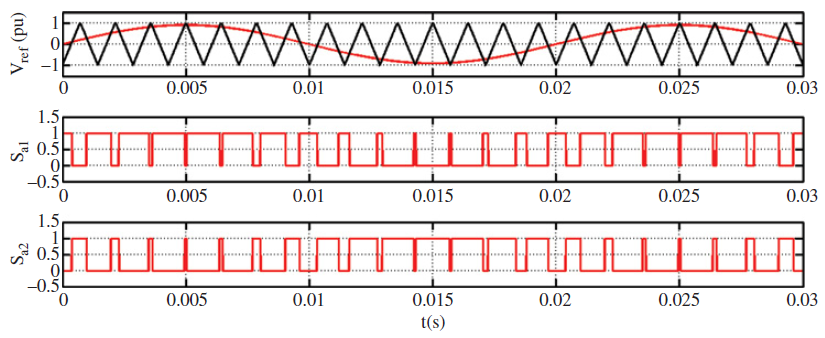
\includegraphics[height = 5.5cm,width = 13.5cm]{Diagrams/Chapter_2/2levelVSC_switching.PNG}
    \caption{SPWM in two-level VSC \cite{noauthor_appendix_2014-1}}
    \label{fig:2levelVSC_switching}
\end{figure}

\subsubsection{Reference frame transformation}\label{ref_frame_trafo}
\gls{PI} controllers are widely used for the control operations in power systems. It is therefore relevant to translate from three-phase abc frame to a rotating \gls{dq} frame in order to have a two signal representation of three-phase \gls{AC} signals. Figure \ref{fig:DQTransformation} shows the Clarke-Park transformation used for this purpose. The three-phase measured signals from the node are translated to a stationary reference frame ($\alpha \beta$) using the Clarke transform. It is then translated to a synchronous rotating \gls{dq} frame using the Park transform. The reference signal for control is provided to the corresponding frame, and after the control process is established, it is translated back to the three-phase signals. In the real scenario, during translation to a rotating \gls{dq} frame, the d-axis is made to align with the voltage of the grid and q-axis is aligned to zero. This approach provides control of active power or \gls{DC} voltage using d-axis current component of the converter, while the reactive power or \gls{AC} voltage can be controlled using the q-axis current component of the converter.   

\begin{figure}[H]
\centering
%\hspace*{-1.2cm}
    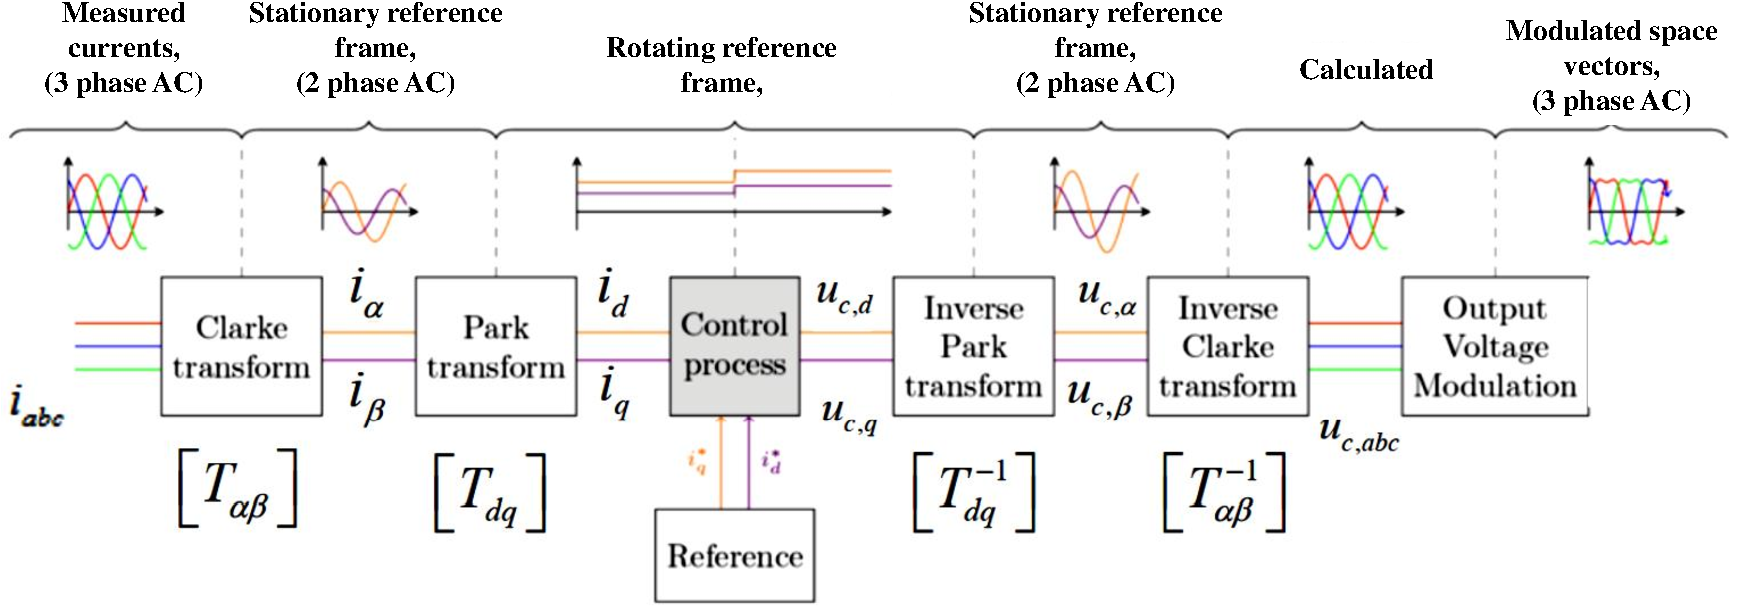
\includegraphics[height = 5.5cm,width = 15.5cm]{Diagrams/Chapter_2/DQTransformation.pdf}
    \caption{Reference frame transformation for control of VSC \cite{ndreko2017offshore}}
    \label{fig:DQTransformation}
\end{figure}

\subsection{Machine Side Converter (MSC) Control}
The \gls{MSC} controller is in charge of optimizing the rotor speed to increase the amount of wind energy being captured continuously \cite{strachan_stability_2010}. There are several control strategies available for achieving different targets \cite{bose_power_2006}. The following equation gives the electromagnetic torque of the \gls{PMSG}.

\begin{equation}\label{elec_torque}
T_e = \frac{3}{2}P_n[\Psi_m.i_q-(L_d-L_q)i_d.i_q]    
\end{equation}

where $P_n$ is the number of pole pairs.


There are majorly three control schemes \cite{wu_variable-speed_2011}:

\begin{itemize}
    \item Zero d-axis Control (ZDC): As the name suggests, this control involves setting the d-axis component of stator current to zero. If $i_d$= 0 in Equation \ref{elec_torque}, the electromagnetic torque will be proportional to the q-axis component of stator current ($i_q$).  
    \item Maximum Torque per Ampere (MTPA) Control: The concept of MTPA control is to generate a required torque with a minimum stator current. On doing so, the use of stator current is increased, and the losses across the stator windings are reduced. In the case of non-salient pole generators, the inductances in d and q axes are the same ($L_d$ = $L_q$). On substituting the same in Equation \ref{elec_torque}, this again simplifies to the fact that electromagnetic torque is proportional to the q-axis current component. Therefore, the MTPA control is the same as the ZDC in case of non-salient pole generators. 
    \item Unity Power Factor (UPF) Control: The stator voltage and current phase angles are calculated initially. To achieve UPF, the angle between the stator voltage and current, i.e. the stator power factor angle must be zero. The equations are then solved for both the d and q axes stator currents, and the constraints are set. 
\end{itemize}

Additionally, the generator is also governed by the Maximum Power Point Tracking (\gls{MPPT}) mechanism to extract the maximum power possible. There are two ways of implementing this mechanism, the first involves measuring the speed of the \gls{WG} shaft, and the maximum mechanical power that can be extracted is calculated. The error obtained by comparing the maximum mechanical power with the actual power achieved is provided for the \gls{MSC} control. The next method is through measurement of wind speed. If for a given speed, the ratio of optimum tip speed ratio and the radius of the blade is known, the optimal rotational speed of the rotor ($v\lambda_{opt}$ /R) can be calculated. The error obtained on comparing this speed with the measured speed is used to calculate the $i_{q,ref}$ component \cite{ali_wind_2012}. The detailed implementation of \gls{MSC} control in RSCAD is given in Appendix[].  

\subsection{Grid Side Converter (GSC) or Line Side Converter (LSC) Control}
The \gls{GSC} is connected back to back with the \gls{MSC} through a \gls{DC} link. The \gls{GSC} is mainly responsible for providing \gls{DC} voltage control and the \gls{AC} side reactive power control. 

\subsubsection{Conventional Current Control}\label{conv_current_control}
The conventional control of \gls{GSC} implemented in power systems follows the current control strategy. This involves an outer loop to control the \gls{DC} voltage ($V_{dc}$) in d-axis, and \gls{AC} voltage ($V_{ac}$) or reactive power ($Q$) control in q-axis as shown in the blue box in Figure \ref{fig:Diss_GSC_control}. The outer loop provides reference set points ($i_{d\_ref}$ and $i_{q\_ref}$) for the inner current control loop which is represented by the red box in Figure \ref{fig:Diss_GSC_control}. The inner loop consists of \gls{PI} controllers and feed-forward term ($V_T$) that form the major part of the control. The decoupling terms ($x$) are added at the end of the current regulator output to improve the dynamic performance of the system.  

The conventional current control strategy has not led to any major issues until now, because the conventional synchronous generators were capable of absorbing the injected currents. However, this is not the case for a network that is dominantly connected using \gls{PE} interface. An example of such a situation is an \gls{OWF} network. The effect could also be severe for a large scale \gls{OWF} network involving more \gls{PE} converters to be connected to the network. Hence this calls for the need for better control strategies.

\begin{figure}[H]
\centering
%\hspace*{-1.2cm}
    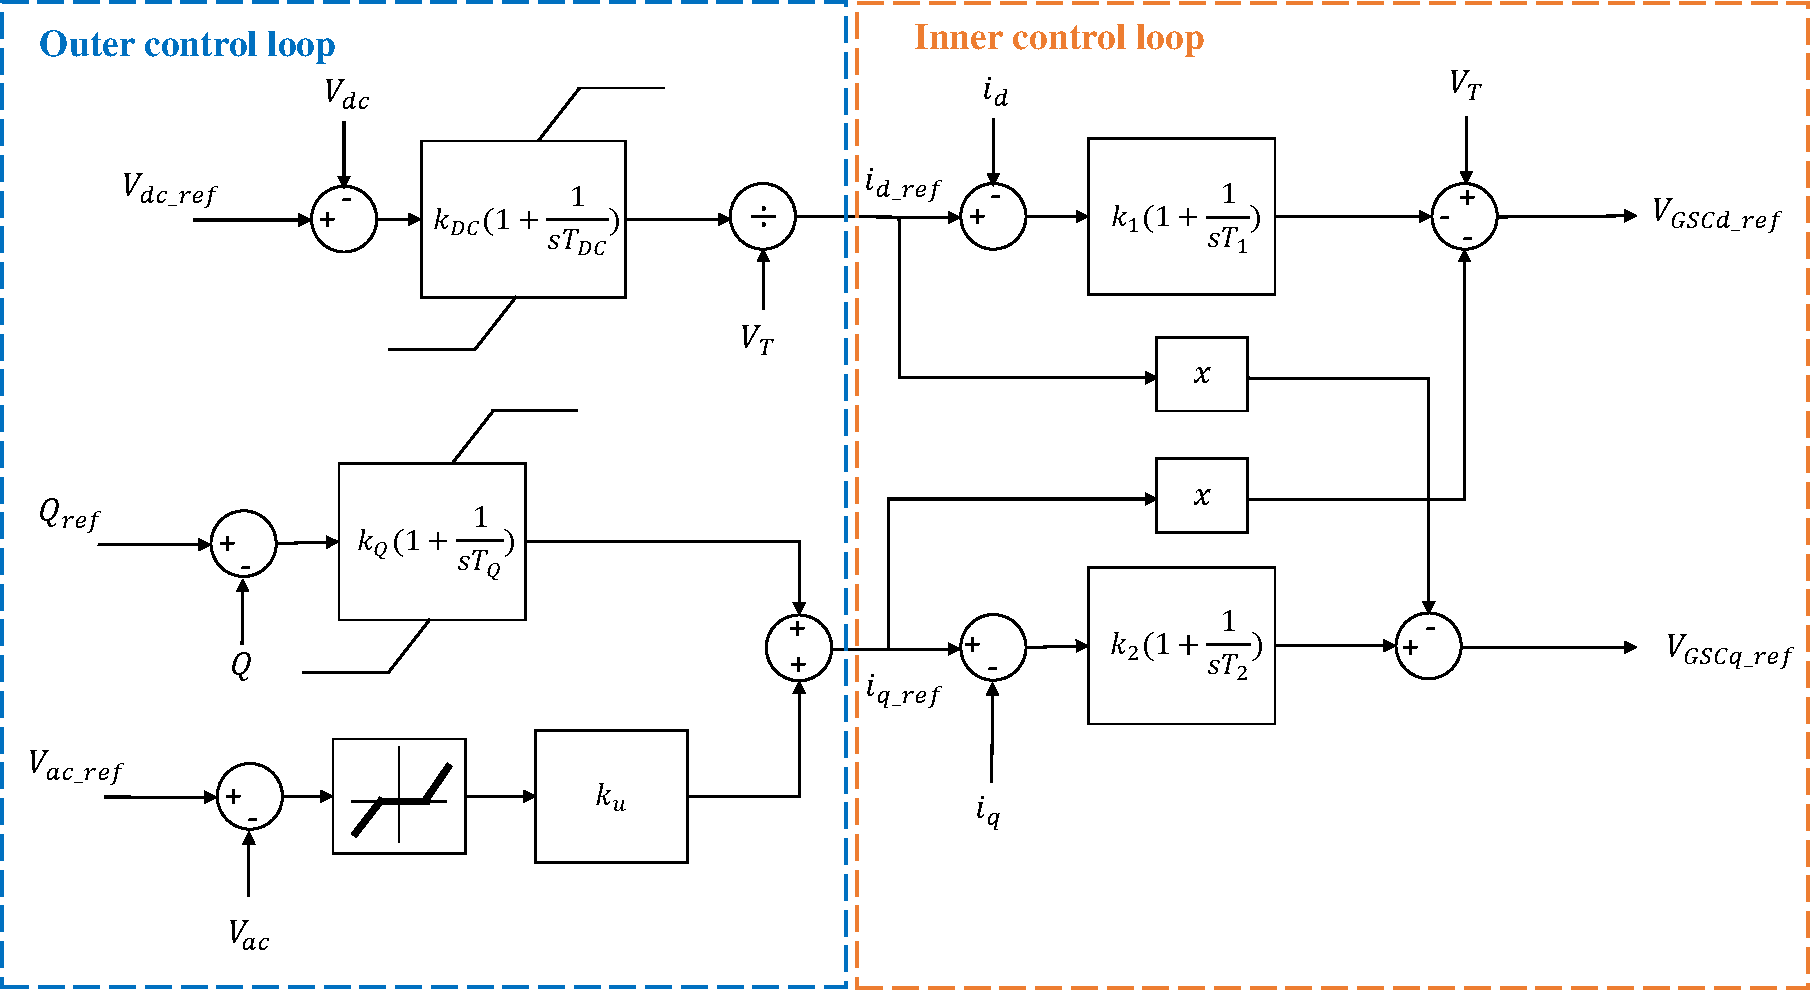
\includegraphics[height = 8.5cm,width = 15.5cm]{Diagrams/Chapter_2/Inner_control_GSC_chap2.pdf}
    \caption{Conventional current control in GSC \cite{korai_dynamic_2019}}
    \label{fig:Diss_GSC_control}
\end{figure}


\subsubsection{Direct Voltage Control (DVC)}\label{DVC_theory}
The major issue with conventional control is the wind up of the integrator that causes the voltage to rise. This happens because the reference value of current remains non-zero and the measured current following islanding nearly falls to zero. To overcome this issue, the inner control loop in Figure \ref{fig:Diss_GSC_control} is modified as shown in Figure \ref{fig:Diss_DVC_control}. In Figure \ref{fig:Diss_DVC_control}, the integrator term is avoided and the proportional term is moved to the output end. However, this causes the set points to be differ in the absence of the integral component. The main role of set points is to limit the \gls{PE} converter current. Nevertheless, the current limitation would be based on the grid situation, and hence the performance of the controller is not affected in the absence of the integral component \cite{korai_dynamic_2019}, \cite{erlich_new_2017}.       

\begin{figure}[H]
\centering
%\hspace*{-1.2cm}
    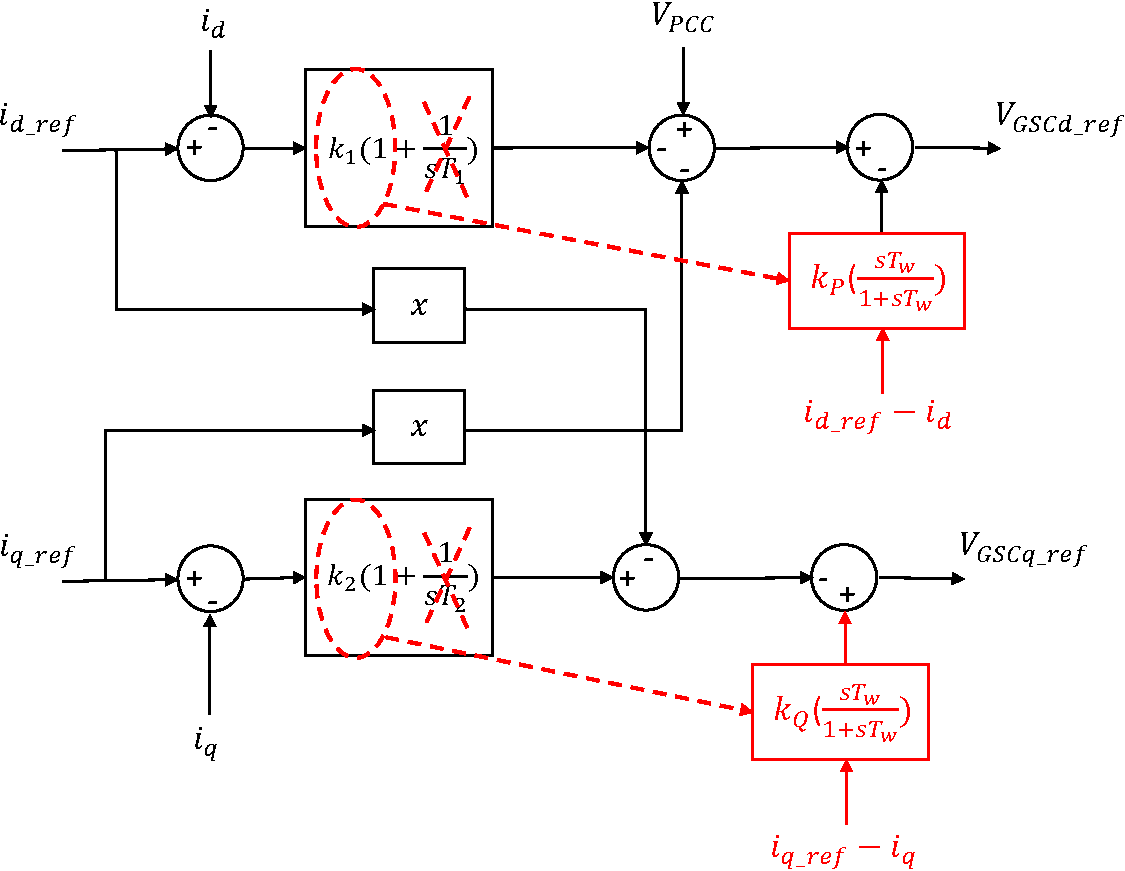
\includegraphics[height = 8.5cm,width = 10.5cm]{Diagrams/Chapter_2/Inner_control_GSC_chap2_2.pdf}
    \caption{ Development of new voltage controller strategy by modifications in the inner control loop of conventional current controller \cite{erlich_new_2017}}
    \label{fig:Diss_DVC_control}
\end{figure}

The damping of transient scenarios is provided by imitating the use of a resistor in series in the \gls{PE} converter circuit. In the real scenario, damping can be depicted as the power loss across a resistor. However, placing a physical resistor in the circuit causes loss of active power which is not desired. In order to achieve the damping effect without power loss, the controller is formulated to mimic the drop in voltage using a virtual resistor \cite{erlich_new_2017}. This is represented by the washout filer depicted in red boxes in Figure \ref{fig:Diss_DVC_control}.

The control strategy developed in \cite{korai_dynamic_2019} uses a vector control strategy similar to the conventional current control. The transformation in d and q axis allows the independent control of active and reactive powers. This control strategy is adapted for this thesis and is explained in detail in Section \ref{DVC_RSCAD}. 

The power balance equation at the \gls{WG} is given as follows:

\begin{equation}\label{powbaleq}
    P_{inverter,input} = P_{rectifier,output} + P_{capacitor}  
\end{equation}

where rectifier is the \gls{MSC} and inverter is the \gls{GSC}. For steady-state conditions, the voltage across the \gls{DC} capacitance is steady. Thereby, the active power input for the inverter (\gls{GSC}) equals the active power output from the rectifier (\gls{MSC}). During the fault condition, the active power output from the inverter is decreased, whereas the output from the rectifier tends to be the same. The capacitors are charged during this scenario, and the \gls{DC} link voltage increases to maintain the power balance. 

\section{High Voltage Direct Current (HVDC) Transmission}\label{HVDC_trans_theory}
As the name suggests, a High Voltage Direct Current (\gls{HVDC}) transmission system uses \gls{DC} for bulk transmission of electrical power. The electrical power from the offshore \gls{AC} network is stepped-up using a power transformer and is converted to \gls{DC} at the converter station which is transmitted to onshore locations using subsea cables or overhead lines \cite{abbreviewnew}. The commercial utilization of \gls{HVDC} transmission was started in 1954 \cite{cigre2005b4}, \cite{peake_history_2010}. The \gls{HVDC} technology employs \gls{VSC}s to convert power from \gls{AC} to \gls{DC} and vice versa as explained in Section \ref{VSC_theory} and hence the systems that employ this technology are termed as \gls{VSC}-\gls{HVDC} systems.

As explained in Section \ref{VSC_theory}, the classification for \gls{VSC}s can be termed as two-level and multi-level. The two-level \gls{VSC}s are an economical solution for low power rating applications up to 1 MVA. The main drawbacks of two-level \gls{VSC}s include increased power losses, high harmonic content on the \gls{AC} side voltages and require expensive filters to mitigate the harmonics. On the other hand, multi-level converters provide notable improvements for the above mentioned issues as can be seen in Figure \ref{fig:2levelVSCtoMMC} \cite{sharifabadi2016design}.   

\begin{figure}[H]
\centering
%\hspace*{-1.2cm}
    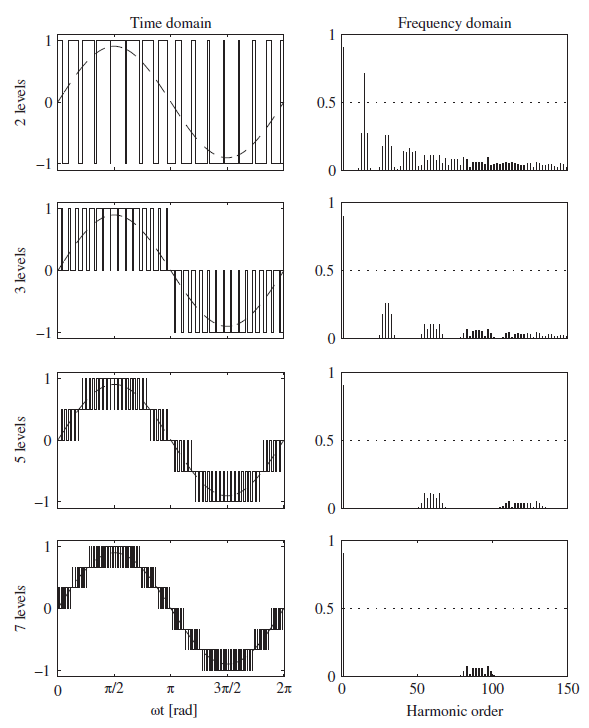
\includegraphics[height = 11.5cm,width = 10.5cm]{Diagrams/Chapter_2/2levelVSCtoMMC.PNG}
    \caption{Effect of moving towards multi-level converters \cite{sharifabadi2016design}}
    \label{fig:2levelVSCtoMMC}
\end{figure}

The most common multi-level converters for high voltage applications in recent times are the Modular Multi-level Converters (\gls{MMC})s. The significant component in an \gls{MMC} is the switching submodule that can be either half-bridge or full-bridge submodules. The half-bridge submodule has one two-level phase leg parallel to a \gls{DC} capacitor that maintains the \gls{DC} voltage. The voltage level can be increased by connecting the submodules in series. The \gls{DC} power at the output of \gls{MMC} is transmitted to the onshore converter using subsea \gls{HVDC} cables. It is converted back to \gls{AC} at the onshore converter station and sent to the distribution network.

Having understood the basics of various equipment in an \gls{OWF} and \gls{VSC}-\gls{HVDC} transmission, the goal of modelling a multi-gigawatt offshore network with identified control strategies needs to be achieved. Implementation of the control strategy for a single \gls{WG} model is taken as the starting step and is explained in the following chapter. 

 \chapter{Modelling and Analysis of DVC in 66 kV HVAC Offshore Network}\label{3}

In this chapter, the basics of Electro-Magnetic Transient (\gls{EMT}) hardware utilized is explained briefly. Then the network model consisting of a Type-4 \gls{WG} with Direct Voltage Control (\gls{DVC}) \cite{korai_dynamic_2019}, \cite{sethi_real-time_nodate-new} in a 66 kV \gls{HVAC} offshore network in RSCAD is detailed. The performance of the control strategy is tested for severe dynamic conditions. Lastly, the performance of the \gls{DVC} modelled in RSCAD is then validated with the benchmark \gls{DVC} model in DIgSILENT PowerFactory software \cite{korai_98_nodate} (based on a qualitative comparison because of the unavoidable differences between the software packages) for a similar 66 kV \gls{HVAC} offshore network.

\section{Real Time Digital Simulator (RTDS) Hardware}\label{RTDS_Theory}
Real Time Digital Simulator (RTDS) Hardware is equipped to perform \gls{EMT} simulation. The overall network solution in RTDS is based on the nodal analysis. The simulator can work in the range from DC to 3 kHz of frequency. It can simulate a time step of 25 - 50 $\mu$s for even complex power systems. This is termed as a large time step. RTDS gives the option for a small-time step environment to incorporate power electronic components simulation. These blocks have time steps in the range of 1400  - 3750 ns. The hardware consists of two generations of processor cards, namely, PB5 and NovaCor \cite{rtds_tech}.  

RTDS provides a user-friendly Guided User Interface (GUI) called RSCAD wherein the network is modelled, run and analyzed. There are modules available in RSCAD for the actions mentioned above (Figure \ref{fig:RSCAD_modules}). These are explained in \cite{rtds_tech} in detail. The majorly used modules for this thesis are the Draft, Runtime, Cable and Tline modules. The modelling of the system is performed in the Draft module, which contains a drawing canvas whose size can be adjusted. The working of the Cable and Tline modules are illustrated in Sections \ref{HVAC_cable_RSCAD} and \ref{Tline_cable_RSCAD}, respectively. Once the model is developed, the simulation is run in the Runtime module. RTDS also allows for Hardware In Loop (HIL) and Software In Loop (SIL) simulations to test the working of controllers in real-world scenario \cite{rtds_tech_hardware}.

\begin{figure}[H]
\centering
%\hspace*{-1.2cm}
    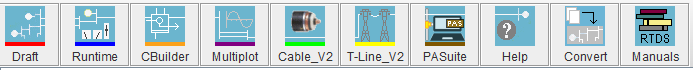
\includegraphics[height = 1.2cm,width = 12.5cm]{Diagrams/Chapter_3/RSCAD_modules.PNG}
    \caption{Modules available in RSCAD}
    \label{fig:RSCAD_modules}
\end{figure}

A simple system model in the Draft module layout is shown in Figure \ref{fig:Dft_RSCAD}. The time step, plot duration and the canvas size is assigned by right-clicking on anywhere on the canvas area and choosing the "Circuit Options" as shown in Figure \ref{fig:Dft_RSCAD}.

\begin{figure}[H]
\centering
%\hspace*{-1.2cm}
    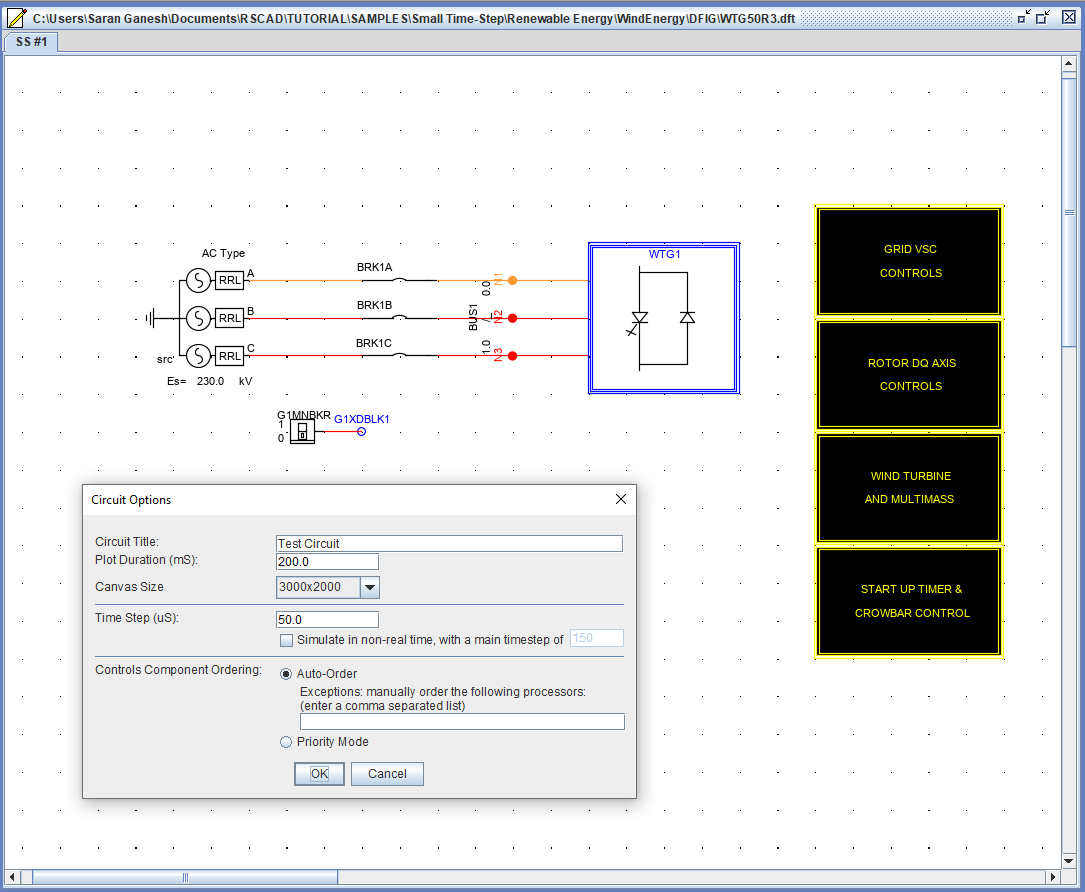
\includegraphics[height = 8cm,width = 10.5cm]{Diagrams/Chapter_3/Dft_RSCAD.PNG}
    \caption{Example of a power system in Draft module in RSCAD}
    \label{fig:Dft_RSCAD}
\end{figure}

There are a variety of libraries available in the Draft module to select the components. The major libraries that were used are \cite{rtds_tech}:
\begin{itemize}\label{Library_RSCAD}
    \item Power system library (Figure \ref{fig:Power_system_lib}) - Consists of power component models such as transformer, transmission line, cables and so forth. These components are to be used in the large time step in the workspace. 
    \item Small time step library - This library consists of components that are used to model in the small-time step environment. The mainly used components are the VSC bridge box, VSC interface transformers, Tline block to interface between small time step and large time step.    
    \item Controls library (Figure \ref{fig:Controls_lib}) - The most important block for modelling control strategies. Consists of transfer functions block, logic functions, math functions and so forth.
\end{itemize}

\begin{figure}[H]
\centering
\begin{subfigure}{.5\textwidth}
  \centering
  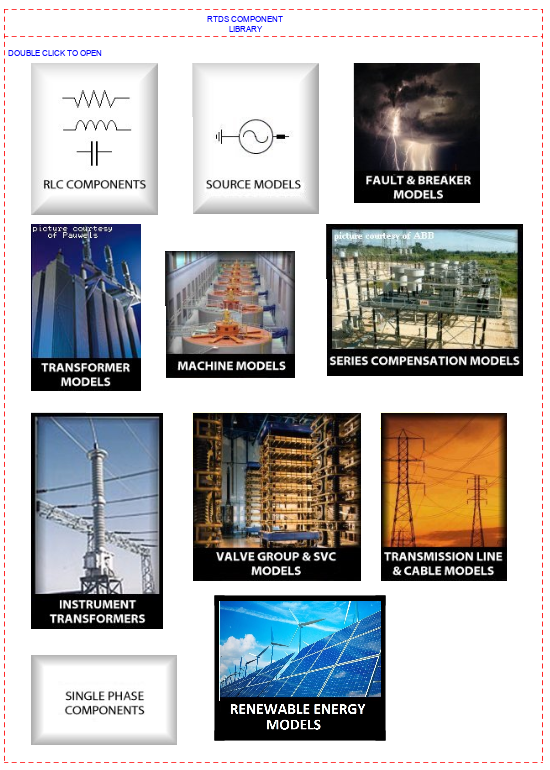
\includegraphics[height=8cm,width=7cm]{Diagrams/Chapter_3/Power_system_lib.PNG}
  \caption{Power system library in Draft module}
  \label{fig:Power_system_lib}
\end{subfigure}%
\begin{subfigure}{.5\textwidth}
  \centering
  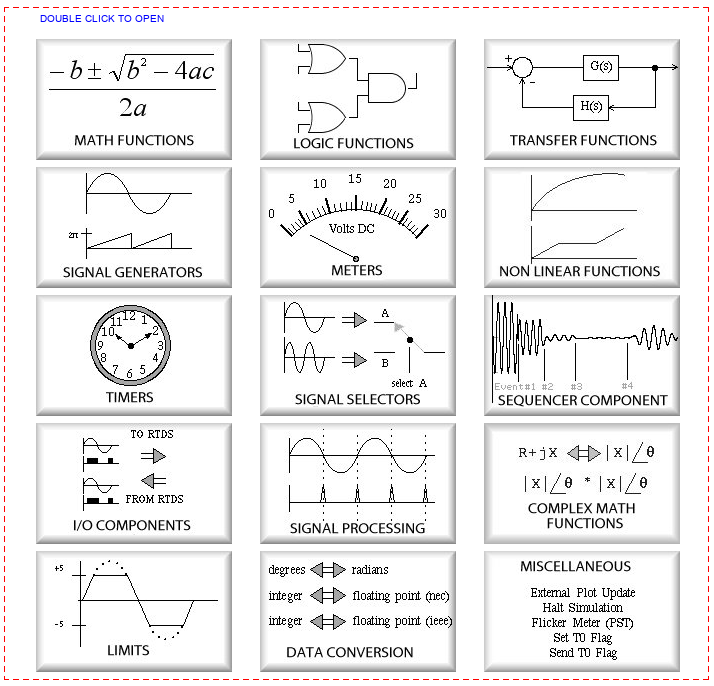
\includegraphics[height=8cm,width=8cm]{Diagrams/Chapter_3/Control_system_lib.PNG}
  \caption{Controls library in Draft module}
  \label{fig:Controls_lib}
\end{subfigure}
\caption{Libraries in the Draft module}
%\label{fig:test}
\end{figure}

After the model has been developed in the Draft module as shown in Figure \ref{fig:Dft_RSCAD}, the user has to compile the file by clicking on "Compile" \footnote{Compile icon in RSCAD: 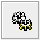
\includegraphics[width=0.6cm, height=0.6cm]{Diagrams/Chapter_3/Compile_pic.PNG}}. The processor calculates the actual time step and along with the initial conditions are stored in the MAP file which is available by right-clicking on the white space in the draft module. The user is notified of errors or warnings during simulation in a pop-up box at the end of file compilation. The processor assignment and the controls assignment can be viewed by clicking the "Processor Assignment" \footnote{Processor Assignment icon in RSCAD 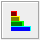
\includegraphics[width=0.6cm, height=0.6cm]{Diagrams/Chapter_3/Processor_assignment_pic.PNG}} tab. There are some important data in the RSCAD configuration files that hold information about the configuration of hardware in RTDS. IP addresses of all rack ports and the processor cards are the data available in the configuration file. It can be accessed using the "Tool" menu in the main tab of RSCAD. Improper configuration of these files will result in no simulation of the test case \cite{rtds_tech}. 

The real-time interaction of the user with the system is done through the Runtime module available in RSCAD. The user can accomplish tasks like measuring signals, plotting graphs, adjusting sliders and creating faults in this interface. An example of the Runtime module with the scenarios mentioned above is shown in Figure \ref{fig:Runtime_RSCAD}.

\begin{figure}[H]
\centering
%\hspace*{-1.2cm}
    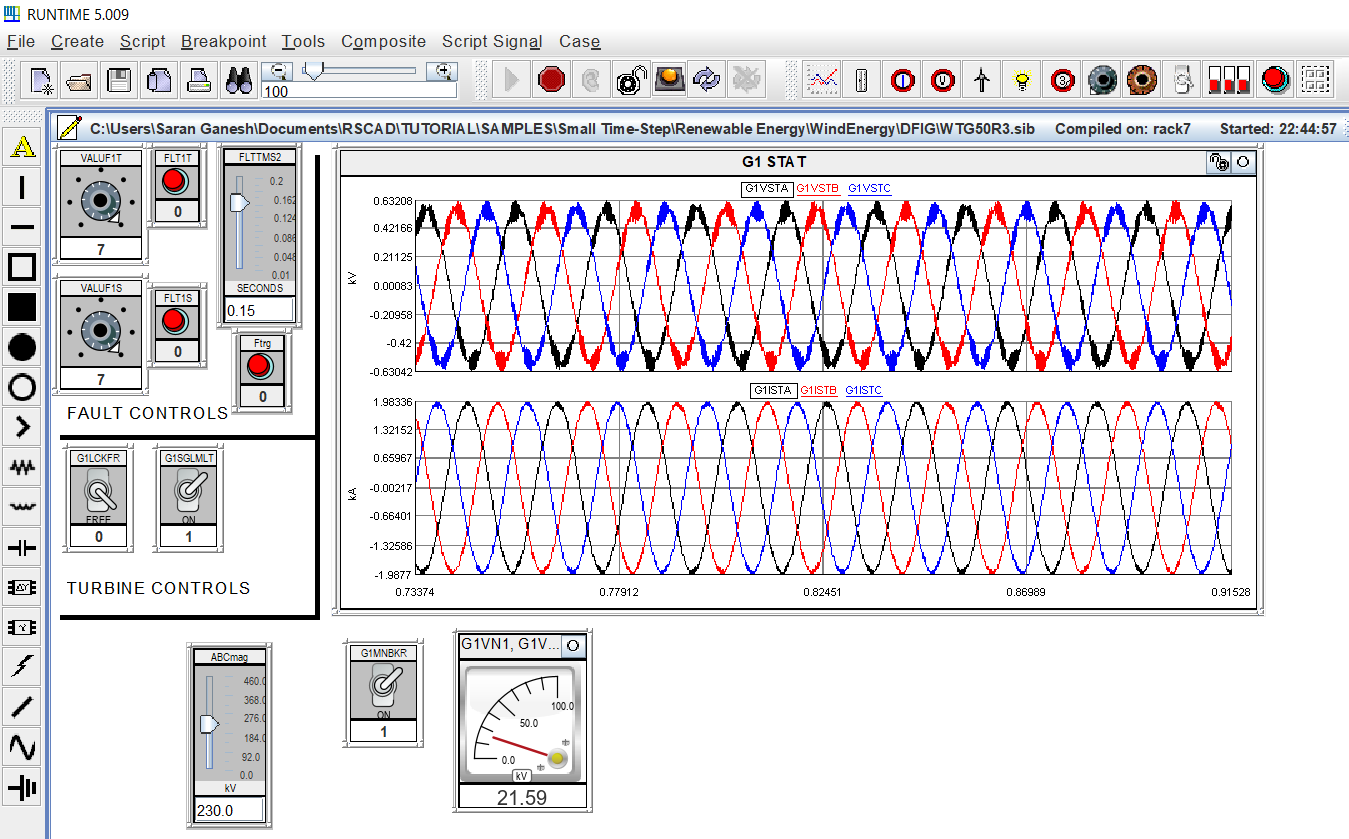
\includegraphics[height = 10cm,width = 15.5cm]{Diagrams/Chapter_3/Runtime_pic.PNG}
    \caption{Example of the Runtime module with plots, switches, sliders etc. in RSCAD}
    \label{fig:Runtime_RSCAD}
\end{figure}



The overall working of RSCAD can be understood as depicted by the flowchart in Figure \ref{fig:RSCAD_Flowchart}.
\begin{figure}[H]
\centering
%\hspace*{-1.2cm}
    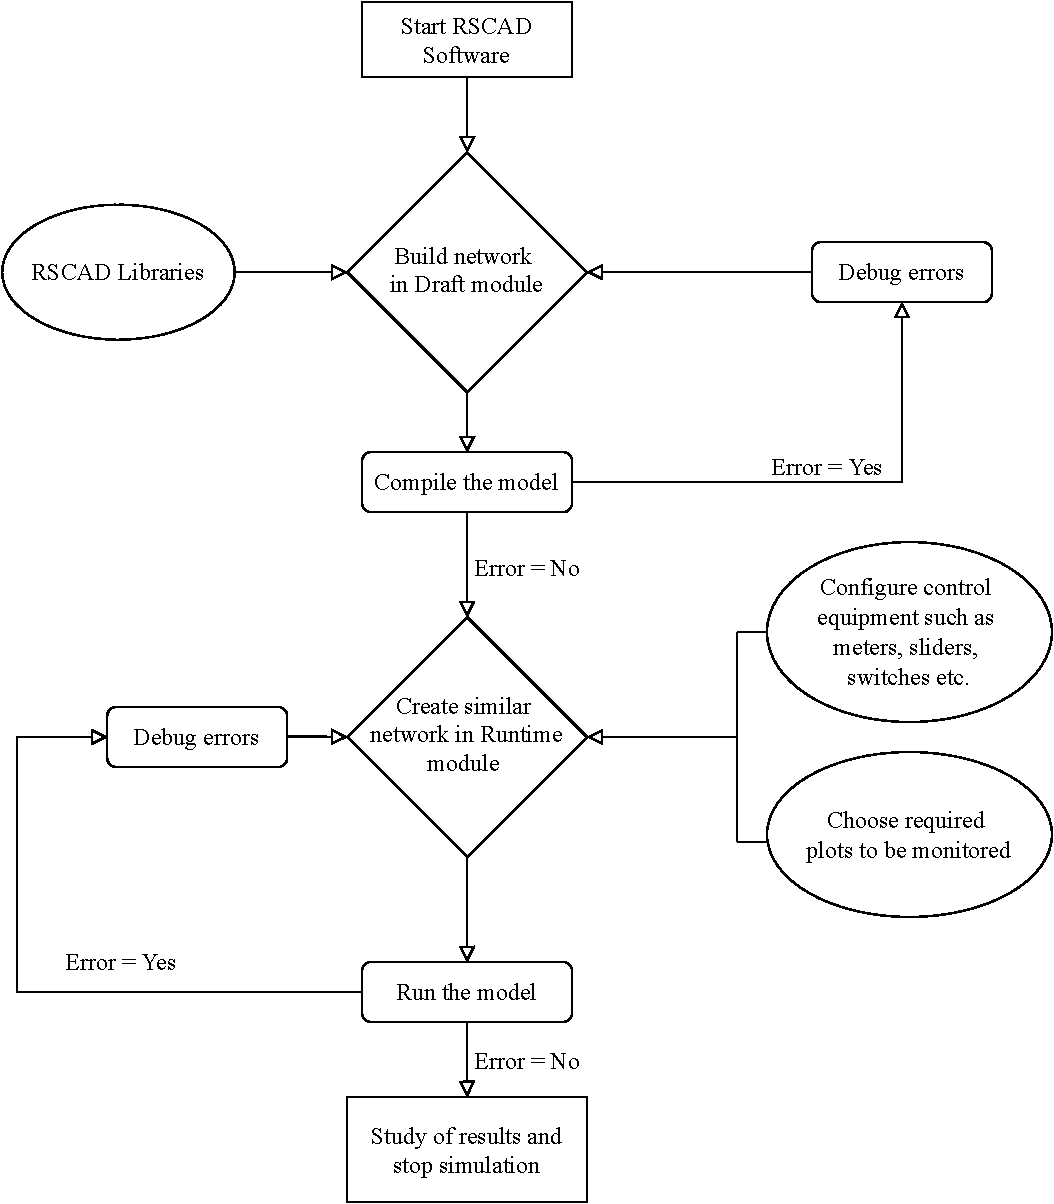
\includegraphics[height = 14.5cm,width = 12.5cm]{Diagrams/Chapter_3/RSCAD_Flowchart.pdf}
    \caption{Flowchart representation of RSCAD working}
    \label{fig:RSCAD_Flowchart}
\end{figure}

\section{Layout of the 66 kV HVAC test system in RSCAD}\label{RSCAD_ACsourcemodel}\label{WT1_ACsource_RSCAD_Test_Layout}
After understanding the basics of RSCAD software, a 66 kV offshore network, as shown in Figure \ref{fig:WT1_Model_RSCAD} is developed. The network consists of the following components.

\begin{itemize}
    \item An aggregated representation of 700 MW installed capacity Offshore Wind Farm (\gls{OWF}) is modelled with the following elements:
    \begin{itemize}
        \item A single Wind Generation System with 
    \begin{itemize}
        \item Permanent Magnet Synchronous Generator (\gls{PMSG})
        \item Machine Side Converter (\gls{MSC})
        \item \gls{DC} circuit
        \item Grid Side Converter (\gls{GSC}) 
    \end{itemize}
        \item High Pass filter (\gls{HPF}) with series reactor
        \item \gls{OWF} transformer
    \end{itemize}
    \item \gls{HVAC} cable  
     \item AC equivalent source representing grid connection
\end{itemize}

\begin{figure}[H]
\centering
%\hspace*{-1cm}
    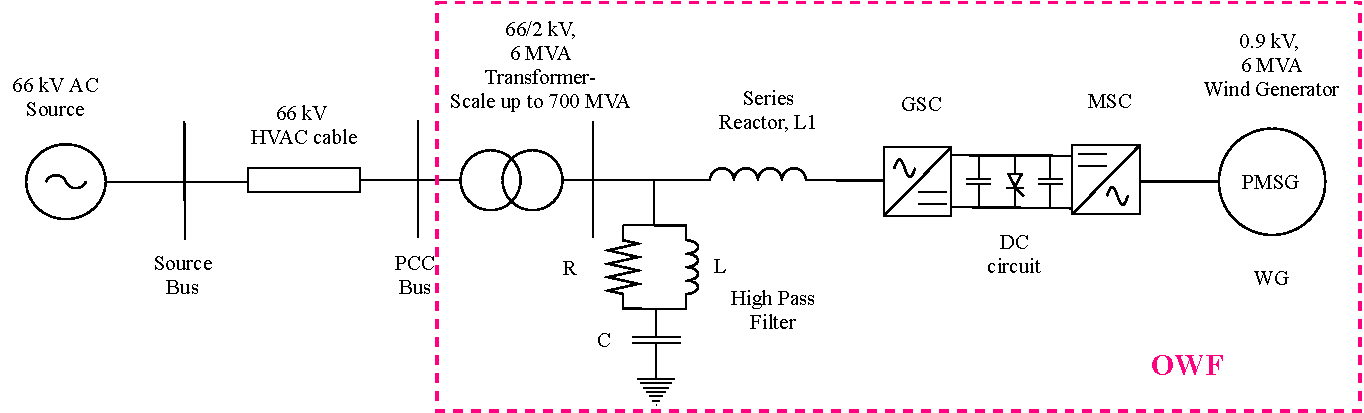
\includegraphics[height = 5.5cm,width = \textwidth]{Diagrams/Chapter_3/WT1_AC_RSCAD_OWF.pdf}
    \caption{Single line diagram of the 66 kV HVAC offshore test network in RSCAD}
    \label{fig:WT1_Model_RSCAD}
\end{figure}

\subsection{ Aggregated Offshore Wind farm (OWF)}\label{OWF}

The 700 MW offshore wind power is represented by a single \gls{OWF} consisting of 116 \gls{WG}s, each rated 6 MW connected in parallel. Type-4 \gls{WG}s are used for all units. The RSCAD representation of aggregated \gls{OWF} is used utilized in this work. The aggregated model consists of \gls{PE} components which require higher switching frequency %(19*50 = 950 Hz in this case) 
and hence is modelled in a small time step environment by selecting the "VSC Bridge Box" (Figure \ref{fig:SmallTimeStepBlock}) available in the small time step library in the Draft module. The box contains the \gls{PMSG}, \gls{MSC}, \gls{DC} capacitors, chopper circuit, \gls{GSC}, high pass filter and offshore transformer as illustrated in Figure \ref{fig:OveriewSmallTimeStepOWF}. As mentioned in Section \ref{RTDS_Theory}, the block can be assigned to have a time step value between 1400 to 3750 ns. 
%It is necessary to set this time step to a nearly high value to avoid the time step overflow error in RSCAD.
The value can be entered by right-clicking on the small time step block and choosing "Edit" and then "Parameters" as shown in Figure \ref{fig:SmallTimeStepBlock}. Also, it must the noted that the above-specified step size is only for initialization and the actual used step size can be viewed in the Map file which is accessible by right-clicking on any white space in the Draft file and selecting "View" then, "Map File". It is also worth mentioning that the ratio of the large time step to the small-time step in a network in RSCAD must be higher than 12 when using NovaCor and must be higher than 17 when using PB5 racks \cite{rtds_tech}. 

\begin{figure}[H]
\centering
%\hspace*{-4.2cm}
    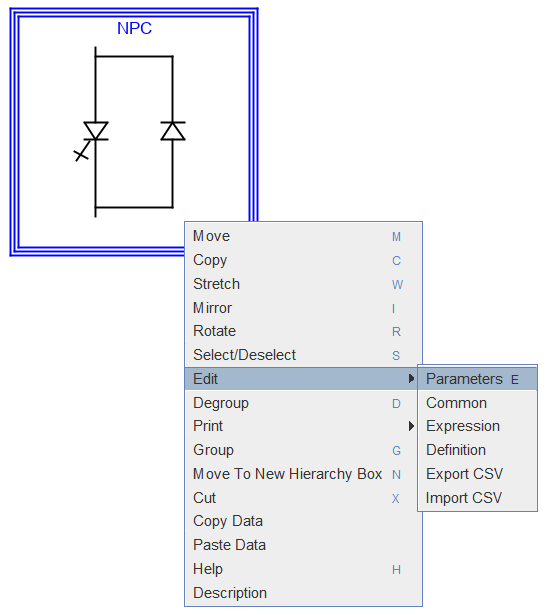
\includegraphics[height = 8cm,width = 7cm]{Diagrams/Chapter_3/SmallTimeStepBlock.PNG}
    \caption{Small time step block}
    \label{fig:SmallTimeStepBlock}
\end{figure}

\subsubsection{Wind Generation System}
The wind generation system consists of \gls{PMSG}, \gls{MSC}, \gls{DC} circuit and \gls{GSC}. Three-level \gls{VSC}s are utilized for the \gls{MSC} and \gls{GSC}. The basic models for this project are considered from the MIGRATE project \cite{denis_migrate_2018}. The detailed description of the \gls{PMSG}, \gls{MSC} and \gls{DC} circuit models along with the control structures are explained in Appendix \ref{Appendix_A}. The control for \gls{GSC} developed in \cite{sethi_real-time_nodate-new} is modified and implemented in this thesis work. This is explained in detail in Section \ref{DVC_RSCAD}.

\begin{figure}[H]
\text{\rotatebox{90}{\hspace{5mm}
\noindent
{\color{magenta} \rule{10mm}{1mm} } \gls{OWF} Transformer
\hspace{15mm}
\noindent
{\color{blue} \rule{10mm}{1mm} } \gls{HPF} with reactor
\hspace{15mm}
\noindent
{\color{green} \rule{10mm}{1mm} } \gls{GSC}
\hspace{15mm}
\noindent
{\color{orange} \rule{10mm}{1mm} } DC Circuit
\hspace{15mm}
\noindent
{\color{yellow} \rule{10mm}{1mm} } \gls{MSC}
\hspace{15mm}
\noindent
{\color{violet} \rule{10mm}{1mm} } \gls{PMSG}}
}
\hspace{10mm}
\centering
%\hspace*{-1.2cm}
    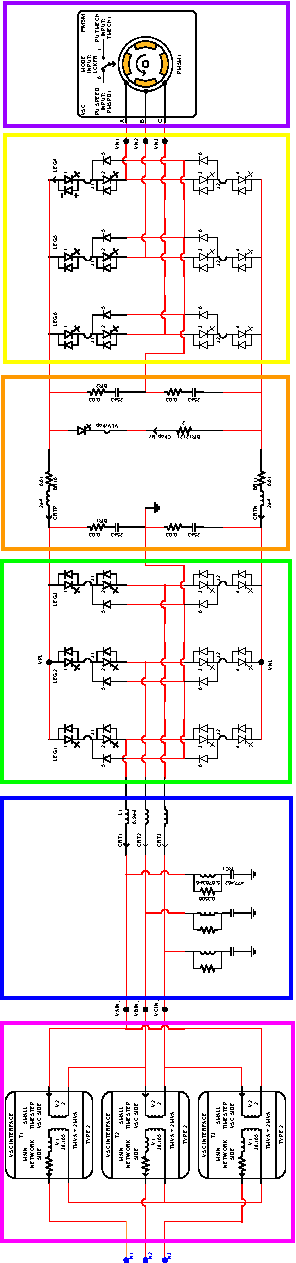
\includegraphics[height = 25cm,width = 6cm]{Diagrams/Chapter_3/SmallTimeStep_WTModel_New3.pdf}
    \caption{Overview of OWF model in small time step environment}
    \label{fig:OveriewSmallTimeStepOWF}
\end{figure}


\subsubsection{High Pass Filter (HPF) with Series Reactor}\label{HPF_design}
The switching operation of converters leads to generation of harmonics. Thereby, to mitigate these harmonics, filters are provided at the output of the \gls{GSC}. There are various types of filters available for this application. The common ones are the LCL filter, L filter and high pass filter \cite{beres_review_2016}. In RSCAD, there is a high pass filter block readily available in the small time step library, as shown in Figure \ref{fig:HPF} \cite{rtds_tech}. It is chosen by selecting the \gls{VSC} branch model in this library and changing the branch type to "HIPASS". A three-phase inductance branch is chosen by selecting the branch type to "L" and connected as the series reactor, as shown in Figure \ref{fig:OveriewSmallTimeStepOWF}. After the \gls{HPF} parameters are calculated and set, then it would only be required to tune the inductance of the series reactor to limit the flow of current by adding impedance and hence stabilizing the voltage. Hence it was decided to go with \gls{HPF}.

\begin{figure}[H]
\centering
%\hspace*{-4.2cm}
    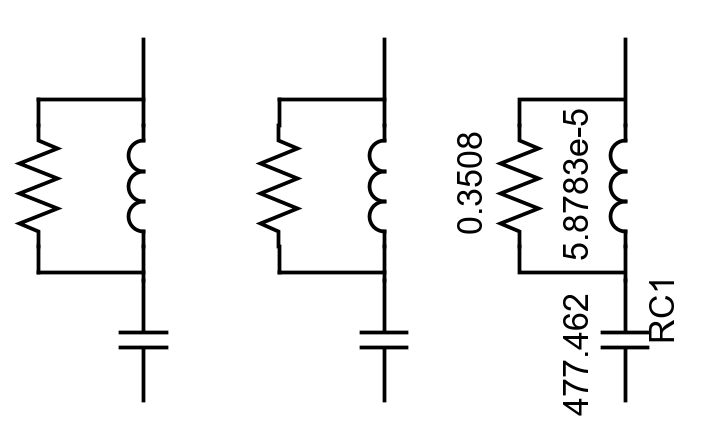
\includegraphics[height = 3.5cm,width = 5cm]{Diagrams/Chapter_3/HPF_RSCAD.PNG}
    \caption{High Pass Filter in RSCAD}
    \label{fig:HPF}
\end{figure}

The base impedance on the low voltage side of transformer is calculated in ohms as in Equation \ref{base_impedance}.
\begin{equation}\label{base_impedance}
    Z_{baseLV} = \frac{LV^2}{Base MVA} = \frac{(2 kV)^2}{6 MVA} = 0.6667\Omega  
\end{equation}

The \gls{HPF} should have a high impedance value at the nominal frequency (50 Hz) so that it works as an open circuit. Therefore, a higher value of 10 times base impedance is chosen. The impedance of the capacitor at 50 Hz is computed by the following equation.

\begin{equation}
    Z_c = 10 * Z_{baseLV} = 10 * 0.6667 \Omega = 6.667 \Omega   
\end{equation}
Hence, the value of capacitance at 50 Hz in Farad is calculated by using Equation \ref{capac_eq},
\begin{equation}\label{capac_eq}
    C = \frac{1}{2\pi f *Z_c} = \frac{1}{2\pi*50 Hz*6.667\Omega} = 4.77462*10^{-4} F
\end{equation}

The next step is to calculate the inductance 'L'. The inductance must be selected so that during the switching or modulating frequency (950 Hz in this case), the impedance of the inductor and capacitor cancel each other. The switching and higher frequencies can be passed to the ground and thereby purely sinusoidal signals will be transferred to the \gls{PCC} on doing so. The impedance of the inductor, resistor and capacitor must be equal at the switching frequency in order to pass the high frequencies to the ground. Therefore, to calculate inductance, it is considered as a series LC circuit. The resonant frequency of the LC circuit is given by Equation \ref{resosn_freq_eq}.

\begin{equation}\label{resosn_freq_eq}
    \omega = \frac{1}{\sqrt{L*C}}    
\end{equation}

Hence, the inductance value can be calculated as per the following equation.

\begin{equation}
    L = \frac{1}{\omega^2*C} = \frac{1}{(2\pi * 950 Hz)^2* 4.77462*10^{-4} F} = 5.8783*10^{-5} H
\end{equation}

Upon deriving the inductance, the resistance is selected to match the impedance of the parallel inductor at the modulating frequency.

\begin{equation}
    R = \omega* L = (2\pi*950 Hz)*5.8783*10^{-5} H = 0.3508 \Omega
\end{equation}

The series reactor is used for limiting the current to the \gls{AC} network. The inductance value of the reactor was selected after precise tuning and is set to 0.9 mH to achieve voltage of 1 p.u. at the \gls{PCC}.

\subsubsection{Offshore Wind Farm Transformer}\label{scaling_OWF}
The \gls{GSC} is connected in series to a three-phase offshore 66/2 kV, 6 MVA transformer through a series reactor and a shunt high pass filter as seen in Figure \ref{fig:OveriewSmallTimeStepOWF}. Single-phase \gls{VSC} interface transformer shown in Figure \ref{fig:VSC_interface_trafo_smalldt} available in the small time step library is used for this approach. Three transformers each rated 2 MVA are connected in delta-wye configuration as seen in Figure \ref{fig:OveriewSmallTimeStepOWF}. In RSCAD, the scaling up of power is done at this transformer. The option for scaling up the primary current of the transformer is available in the \gls{VSC} interface transformer block as shown in Figure \ref{fig:VSC_interface_trafo_scaling} \cite{rtds_tech}. The user can control the amount of scaling, i.e. the number of parallel units by a slider, as shown in Figure \ref{fig:scaling_factor_RSCAD}. The user can model the components in the secondary side of the transformer as required for a single \gls{WG} and then scale it to the required power (700 MW in this case).

\begin{figure}[H]
\centering
%\hspace*{-4.2cm}
    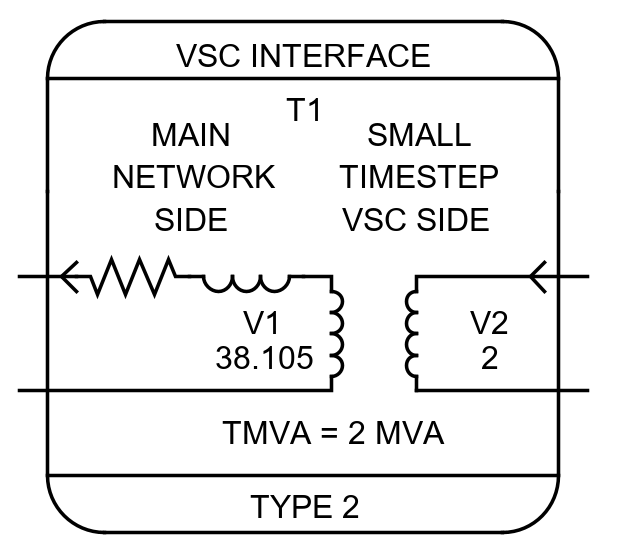
\includegraphics[height = 4cm,width = 4.5cm]{Diagrams/Chapter_3/VSC_interface_trafo_smalldt.PNG}
    \caption{VSC Interface Transformer}
    \label{fig:VSC_interface_trafo_smalldt}
\end{figure}
\vspace{0 mm}
\begin{figure}[H]
\centering
\begin{subfigure}{.55\textwidth}
  \centering
  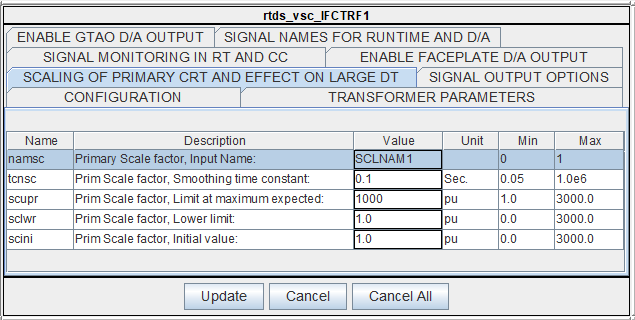
\includegraphics[height=5cm,width=10cm]{Diagrams/Chapter_3/VSC_interface_trafo_scaling.PNG}
  \caption{Option for scaling in VSC transformer}
  \label{fig:VSC_interface_trafo_scaling}
\end{subfigure}%
\begin{subfigure}{.5\textwidth}
  \centering
  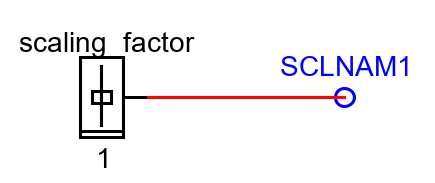
\includegraphics[height=2cm,width=4.5cm]{Diagrams/Chapter_3/scaling_factor_RSCAD.PNG}
  \caption{Scaling factor}
  \label{fig:scaling_factor_RSCAD}
\end{subfigure}
\caption{Scaling up of power in RSCAD}
\label{fig:VSC_trafo_options}
\end{figure}

\subsection{HVAC Cables}\label{HVAC_cable_RSCAD}
The \gls{HVAC} cables transfer power from the \gls{OWF} transformer to the  equivalent 66 kV \gls{AC} source. The \gls{HVAC} cables are rated at 66 kV and modelled in the large time step environment. When compared to 33 kV \gls{HVAC} cable system, 66kV cables allow twice the amount of power to be transferred for the same area of cross-section and require lower array cabling \cite{dnv66kv}. 
 
RSCAD allows cables to be modelled as Frequency Dependent Phase, Bergeron and Pi models \cite{rtds_tech}. The Frequency Dependent Phase and the Bergeron are travelling wave models. Pi model representation of cable is chosen for this research in RSCAD. To ease the goal of comparing the performance of models in two \gls{EMT} software which is shown in the later section, a Pi cable model was chosen. In RSCAD, cable parameters can be entered using the cable module available in the RSCAD modules section as denoted by a red box in Figure \ref{fig:CableModule_mark}. 

 
In the Draft module, the cable model is added in the circuit using the unified model shown in Figure \ref{fig:CableParaBlock} available in RSCAD library. The unified model consists of the following components: 
%\setlist{nolistsep}
    \begin{itemize}[noitemsep]
    \item Calculation Block
    \item Sending End Terminal
    \item Receiving End Terminal
\end{itemize}

The detailed representation of the cable parameters in Cable module, and the representation of the cable model using the calculation block, sending end terminal and receiving end terminals in the Draft module is shown in Appendix \ref{config_cable}.

%\vspace{-13mm}
\begin{figure}[H]
\centering
%\hspace*{-1.2cm}
    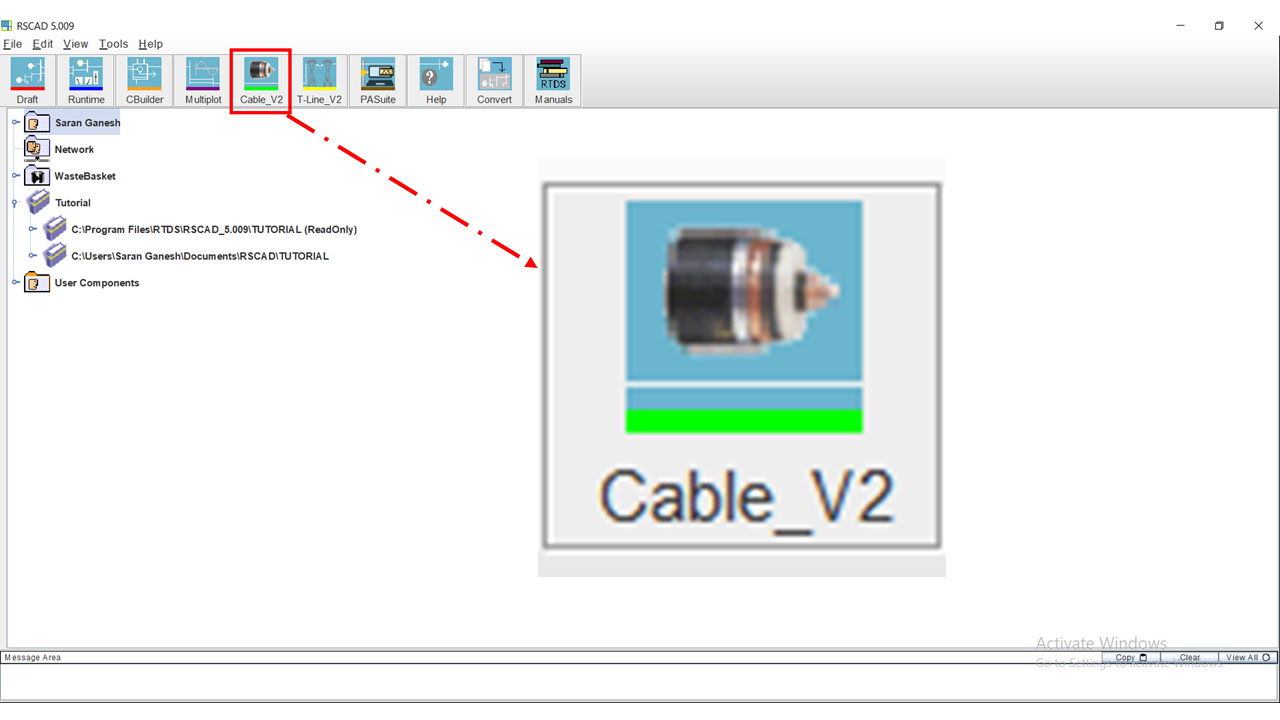
\includegraphics[height = 4.5cm,width = 7.5cm]{Diagrams/Chapter_3/Cable_module_Final.png}
    \caption{Cable module in RSCAD}
    \label{fig:CableModule_mark}
\end{figure}
%\vspace{-16mm}

\begin{figure}[H]
  \centering
  % include first image
  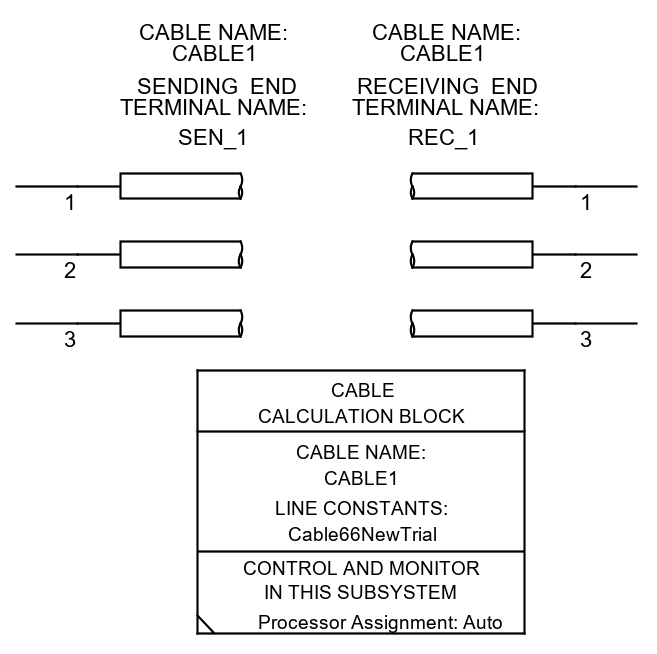
\includegraphics[height = 6cm,width = 6.5cm]{Diagrams/Chapter_3/CableParaBlock.PNG}  
  \caption{Cable configuration}
  \label{fig:CableParaBlock}
\end{figure}

\subsection{External AC system}\label{ext_AC_source}
The external \gls{AC} system represents the infinite grid connection and is modelled as an \gls{AC} voltage source. The infinite grid representation is similar to the representation of a synchronous generator with high inertia constant. For a strong grid, typical values of inertia constant of 5 MW/MVA$^2$ depicting a synchronous generator is chosen from \cite{kothari2003modern}. The commonly represented damping constant is the frequency-dependent load damping constant. However, the damping constant is zero in this case as no loads and a lossless machine is considered. Alternatively, for short circuit calculations, the reference parameters given in \cite{wachal2014guide} can be chosen for representing a infinite grid. The parameters include short circuit power of 30 GVA and X/R of 10. The \gls{AC} source voltage is rated at 66 kV (line-line RMS).

\section{Control structures}
The control strategies are implemented in the \gls{MSC} and \gls{GSC} of the \gls{WG}. The decoupled current control architecture utilized in \gls{MSC} is explained in Appendix \ref{MSC_Control}. The major area of interest for this thesis is the control strategy of \gls{GSC}. The \gls{DVC} illustrated in Section \ref{DVC_theory} is implemented in the \gls{GSC}.   

\section{Implementation of DVC in RSCAD}\label{DVC_RSCAD}
The control strategy depicted in \cite{korai_dynamic_2019} is achieved in RSCAD software. The control was implemented in RSCAD in \cite{sethi_real-time_nodate-new} for a 33 kV transmission network, but the final goal of achieving reactive current injection during severe dynamic conditions was lacking. The primary reason was due to the current limiter block that is explained later in this section. The block is implemented successfully in this work, and the results are illustrated. 
As RSCAD allows modelling of the secondary side of the transformer as required for one \gls{WG}, the control loop parameters of \gls{GSC} remain the same as 33 kV for a 66 kV offshore network and are based on the benchmark values provided in \cite{korai_98_nodate}. The control strategy described in Section \ref{DVC_theory} is incorporated in the reactive power and active power control loops defined in the following section. 

\subsection{Reactive Power Control}
From the control structure, it can be seen that, unlike in conventional current control, the reactive current is not directly utilized for voltage control. The converter voltage is directly controlled here, and this allows the current to modify on its own according to varying network conditions. This strategy is similar to the voltage control in conventional synchronous generators. The reactive control loop consists of an outer loop based on a slow VAR controller that tracks the changes in set-points required by the system-wide demand. The inner loop consists of a fast-acting controller, as the name suggests, that responds towards crucial changes in voltage where quick action is required \cite{korai_dynamic_2019}.

\begin{figure}[H]
\centering
%\hspace*{-1.2cm}
    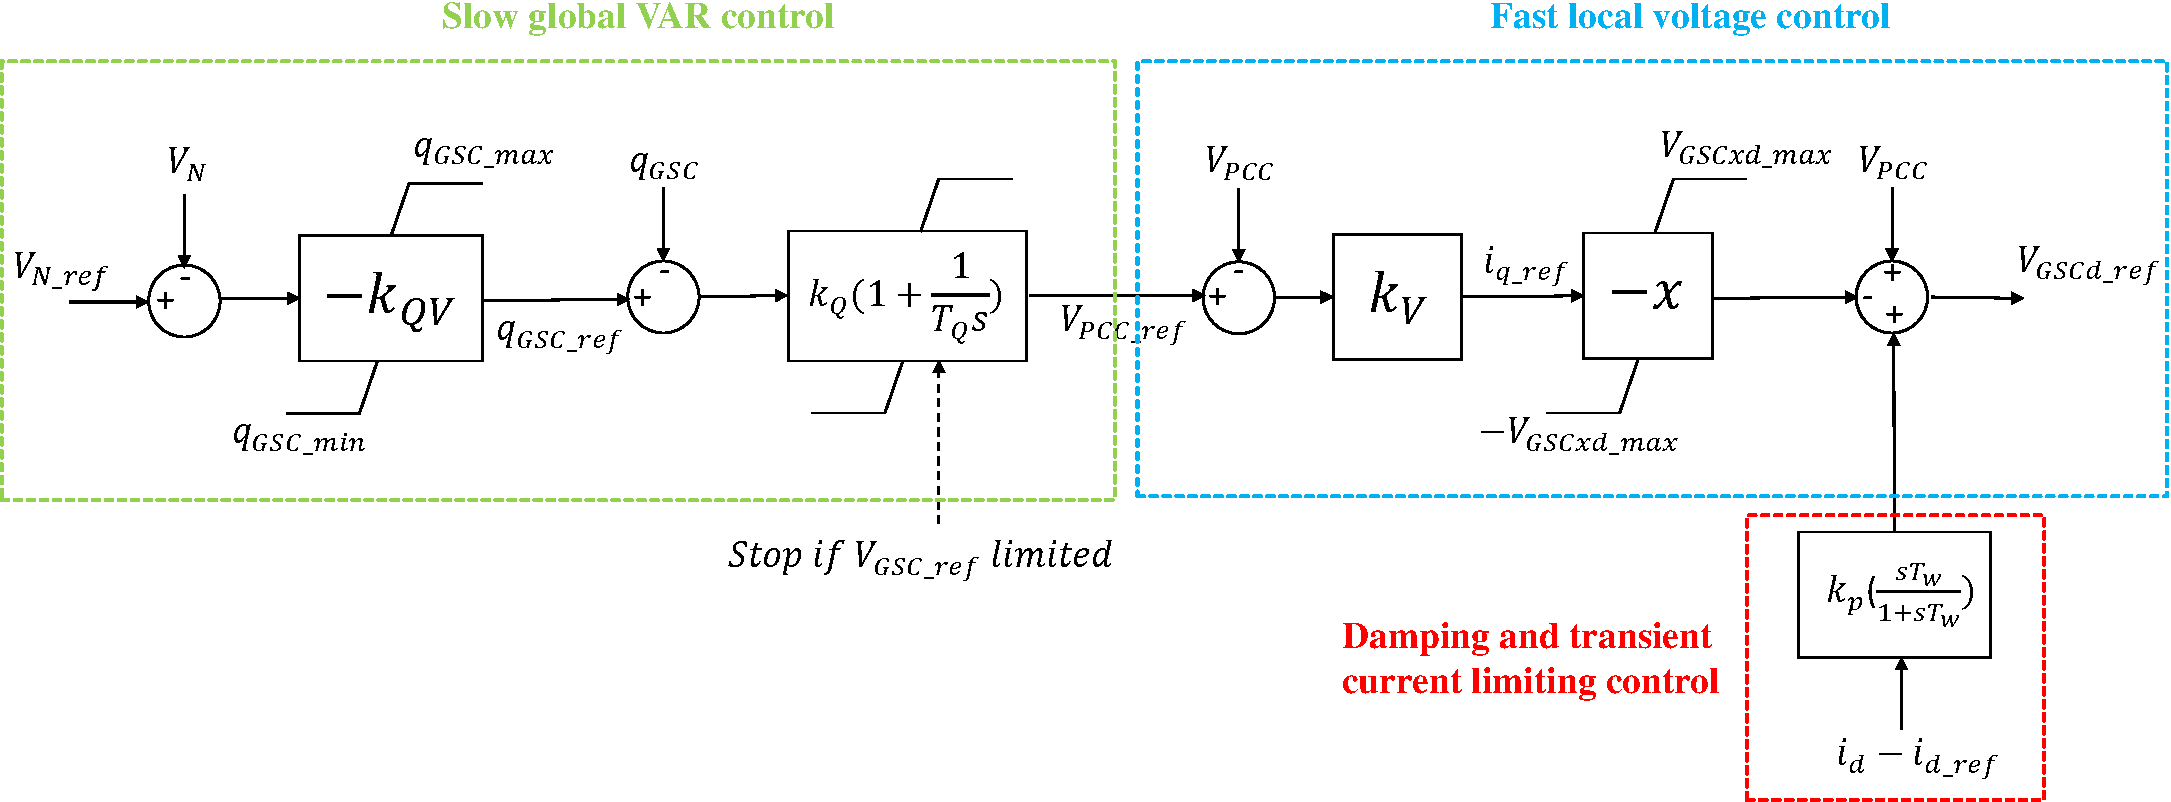
\includegraphics[height = 6.5cm,width = \textwidth]{Diagrams/Chapter_3/Reactive_power_loop.pdf}
    \caption{Reactive Power control loop \cite{korai_dynamic_2019}}
    \label{fig:Reactive_Power_Control_Loop}
\end{figure}

\paragraph{Slow global VAR control}
It is the upper-level controller and can be modelled as a power factor, reactive power or voltage controller. The reference values can be directly sent as inputs to the \gls{PI} controller if the controller is made to use for reactive power or power factor control. The voltage controller is used here, and this requires reactive power reference to be determined from a predefined voltage versus reactive power droop characteristic. A voltage value for which the injection of reactive power is zero is obtained from this characteristic. The obtained reactive power reference output is provided as input to the \gls{PI} controller having a small proportional gain and ample time constant in order to avoid transformer tap changes and not very fast in order to avoid unwanted controller interactions. The automatic adjustment of reactive power in relation to varying voltage using the proportional gain $k_{QV}$ is significant. There is no dead-band present in order to ensure continuous voltage control. The  proportional gain that represents the droop can be obtained from the following relation,

\begin{equation}
    k_{QV} = \frac{\Delta q_{gsc}}{\Delta V_N}
\end{equation}

In theory, the proportional gain can be varied with changes in power flow. But this is not practically feasible and hence it is recommended to set the reactive power reference ($q_{ref}$) based on load flow calculation in the network and corresponding optimum power flow (OPF) calculations. The values could be updated at regular intervals. $V_{N\_{ref}}$ can be determined from $q_{vsc\_ref}$ as,
\begin{equation}
    V_{N\_{ref}} = -\frac{q_{vsc\_ref}}{k_{QV}} + V_N
\end{equation}
where $V_N$ is desired voltage and $V_{N\_{ref}}$ is the voltage at which no reactive power injection is required.
The reactive power limits $q_{vsc\_max}$ and $q_{vsc\_min}$ are the continuous values in steady-state and can be computed from the P-Q diagram of the converter operation. The time constant is chosen in the range of 5-30 seconds wherein a value in the higher range tends to stabilize whereas a value in the lower range can cause interactions with other controllers.

The slow global VAR controller must be made inactive once the converter current limit is reached and also during cases of large voltage sags or swells by providing a signal to deactivate the controller. A scenario that could lead to the case mentioned above is a three-phase short circuit event. The output from the upper-level controller must be constant because of the chosen high integration time constant or must be limited by a blocking signal \cite{korai_dynamic_2019}.

\paragraph{Fast local voltage control}
The terminal voltage reference output received from the slow global VAR controller is provided as input to the fast local controller. This controller must be able to provide prompt support for grid voltage during the time of faults. The response of the controller in terms of voltage support must depend on local inputs sensed at the \gls{PCC} and not on quantities that need to be measured at remote places using a communication mechanism. A proportional gain is used for this purpose. The proportional gain can be obtained from the following relation \cite{korai_dynamic_2019},

\begin{equation}
    k_V = \frac{\Delta i_{Q\_vsc}}{\Delta V_N }
\end{equation}

The primary control action is provided by the feed-forward term, $x$, which is the reactance of the \gls{PE} converter. The voltage output obtained on multiplying the current with $x$ is the set point voltage of the converter in steady state.

\subsection{Active Power Control}\label{Active_power_DVC_theory}
The active power control consists of the \gls{DC} voltage, direct frequency control and Voltage Dependent Active Power Reduction (VDAPR) control, as shown in Figure \ref{fig:Active_Power_Control_Loop}. The control of active power is provided using the q-axis component of \gls{GSC} voltage as per the Equation \ref{P_eq}. Practically, since the \gls{DC} capacitor provides the active power control, the \gls{DC} energy barrier should be made higher which is to be done by increasing the capacitor size and \gls{DC} voltage when in comparison with the conventional \gls{PI} based current control \cite{korai_dynamic_2019}. One modification that was done is providing the minimum limit, $V_{a\_lim\_min}$, for the voltage measurement. A small value needs to be set for this parameter since in RSCAD software without a minimum limit, an error causing division by zero would be bound to occur during the start of the simulation. 

\begin{equation}\label{P_eq}
    p = V_Ti_d = -V_T\frac{v_{conv,q}}{x}
\end{equation}
where $V_T$ is the voltage at \gls{PCC}.

The direct frequency control provides control in case of under frequency and over frequency. The control is modelled to be activated when the frequency is above 50.2 Hz or below 49.8 Hz.
The VDAPR control is provided to control the power injection capacity of the \gls{GSC}. Since power cannot be injected to the grid by the \gls{GSC} during the time of faults, the VDAPR allows in reducing the set point of reference power and thereby refining the dynamic stability of the network. 
\begin{figure}[H]
\centering
%\hspace*{-1.2cm}
    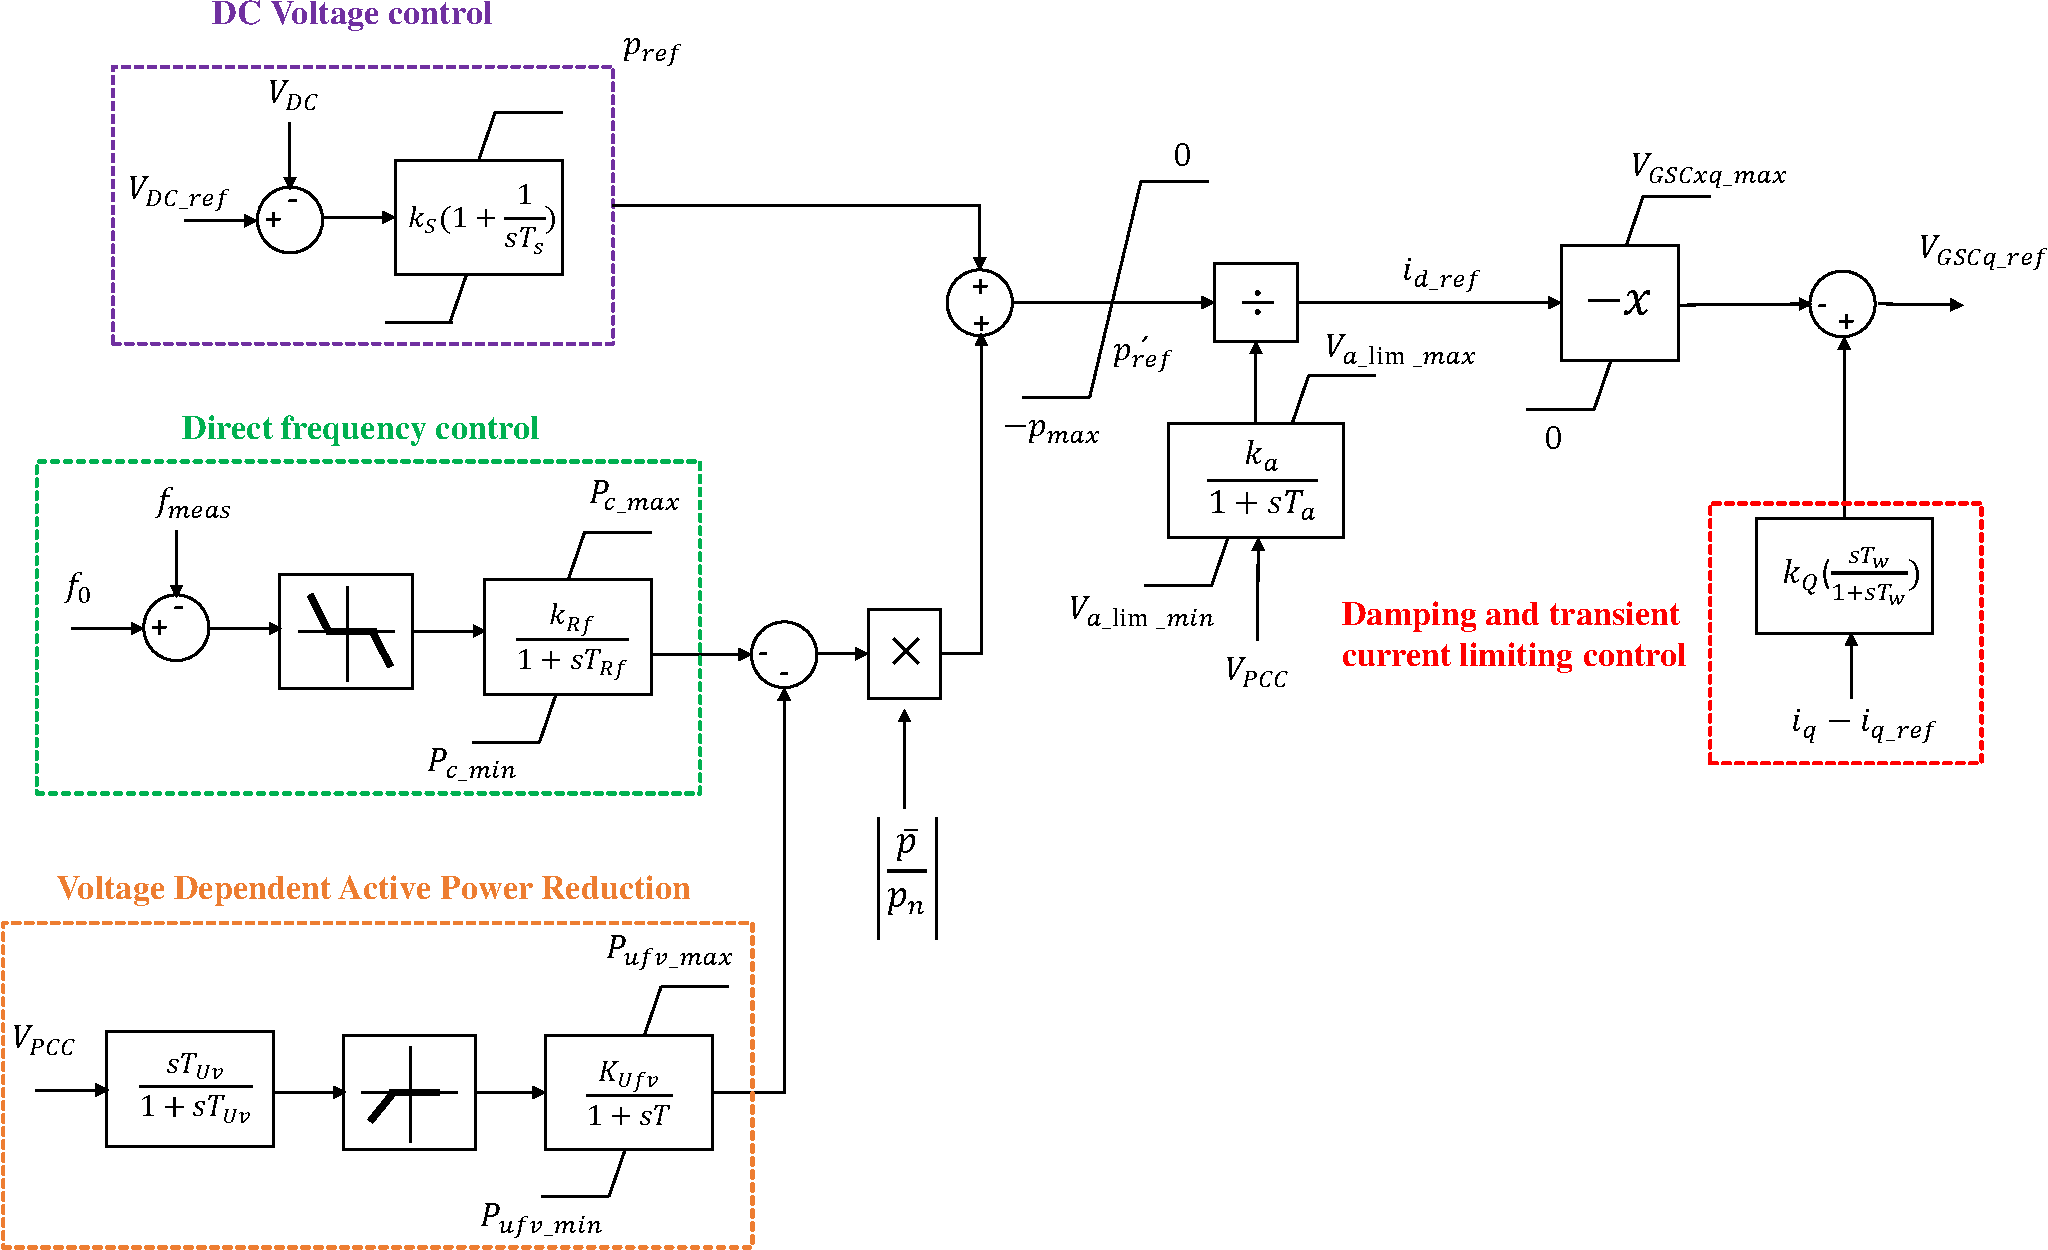
\includegraphics[height = 12cm,width = \textwidth]{Diagrams/Chapter_3/Active_power_loop_withfreq.pdf}
    \caption{Active Power control loop \cite{korai_dynamic_2019}}
    \label{fig:Active_Power_Control_Loop}
\end{figure}

\subsection{Current Limitation}\label{currentlimitation_RSCAD}
The current limitation is an important block that protects the \gls{PE} components from damage due to over current. A new maximum current value is computed whenever the maximum current of the \gls{PE} converter is exceeded. The current limitation is incorporated in \gls{GSC} based on Equations \ref{currentlimeq1} and \ref{currentlimeq2}. The upper and lower limits for $i_{q\_ref}$ and $i_{d\_ref}$ are calculated based on the grid impedance and the new computed maximum current value, as shown in Figure \ref{fig:Current_Limiter_block}. 
Once the reference limits are computed, the converter voltage limits are calculated by Equation \ref{vol_lim_1} or by Equations. \ref{vol_lim_2} and \ref{vol_lim_3} \cite{korai_dynamic_2019}.

if
\begin{equation} \label{currentlimeq1}
% \begin{split}
  (|i_d+ji_q|-i_{max0\_ref})>0 \longrightarrow i_{max\_ref} = i_{max0\_ref} - k_{red} .(|i_d+ji_d|-i_{max0\_ref}) \\
\end{equation}

else
\begin{equation}\label{currentlimeq2}
    \\
  i_{max\_ref} = i_{max0\_ref}  
% \end{split}
 \end{equation}
 
\begin{figure}[H]
\centering
%\hspace*{-1.2cm}
    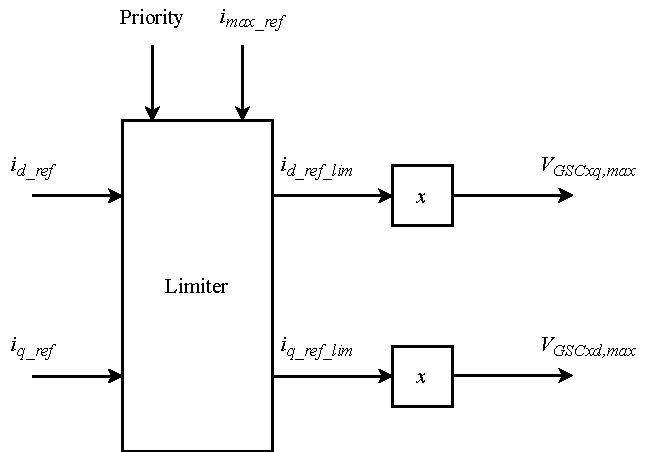
\includegraphics[height = 7.5cm,width = 10cm]{Diagrams/Chapter_3/Current_Limiter_block.pdf}
    \caption{Current limitation algorithm in VSC \cite{korai_dynamic_2019}}
    \label{fig:Current_Limiter_block}
\end{figure}

As long as the reference current is not limited,
\begin{equation}\label{vol_lim_1}
    V_{GSCqx,max} = V_{GSCdx,max} = x . i_{max,ref}
\end{equation}

else

\begin{equation}\label{vol_lim_2}
    V_{GSCqx,max} = x . i_{d\_ref\_lim} 
\end{equation}
\begin{equation}\label{vol_lim_3}
    V_{GSCdx,max} = x . i_{q\_ref\_lim}
\end{equation}

\subsection{Voltage Limitation}
The \gls{AC} voltage of the \gls{GSC} is generally limited by the \gls{DC} voltage value. The factor that brings the relationship between the \gls{AC} and \gls{DC} voltages is the modulation index. The modulation index is computed, as shown in Equation \ref{MI_eq}. The maximum value of the modulation index is set around to 1, and \gls{GSC} voltage must be limited at that point to avoid non-saturation of the \gls{GSC}. 

\begin{equation}\label{MI_eq}
    m = \frac{2\sqrt{2} V_{AC}}{\sqrt{3} {V_{DC}}}
\end{equation}

\section{Analysis of the dynamic performance of 66 kV test system}
After the 66 kV system is modelled, it has to be tested for operation in steady-state and dynamic conditions. The performance related to voltage restoration and reactive power injection by the \gls{DVC} during the worst dynamic situation in the grid has to be analyzed. A three-phase short circuit in the middle of the \gls{HVAC} cable is chosen to test the same.

\subsection{Three-phase line to ground fault}

The line to ground fault logic available in the power system library in RSCAD is adapted in this network by splitting the cable model into two halves and connecting it in the middle of the two halves of the cables as shown in Figure \ref{fig:2cablesblockwithfault}. The fault logic is explained in Appendix \ref{fault_logic}. 
The Draft module is compiled, and after ensuring no errors, the system is run in the Runtime module. The system is stabilized with the voltage values within the tolerance limit of $\pm$ 10\% during steady-state operation.

\begin{figure}[H]
\centering
%\hspace*{-1.2cm}
    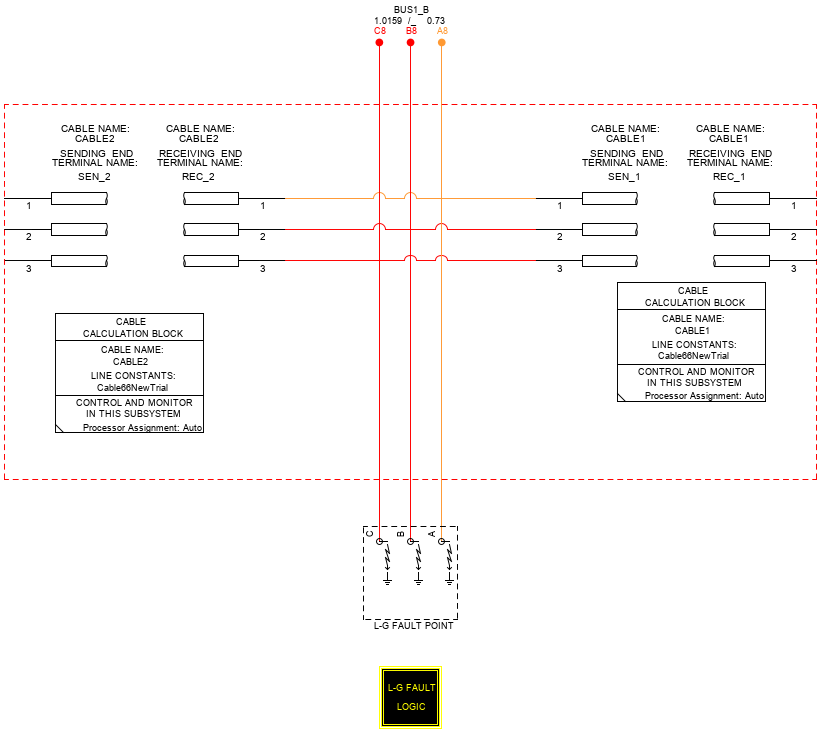
\includegraphics[height = 11.5cm,width = 12.5cm]{Diagrams/Chapter_3/2CablesBlockWithFault.png}
    \caption{Representation of three-phase fault in the middle of the cable in RSCAD}
    \label{fig:2cablesblockwithfault}
\end{figure}

The three-phase line to ground fault is applied at 0.5 s with a fault clearing time of 140 ms. The voltage and frequency responses are as shown in Figure \ref{fig:Vol_Freq_3phaseSC}. In the pre-fault condition, the voltage is stabilized and the active current of nearly 1 p.u. is provided by the \gls{GSC}. There is no reactive current or reactive power injection during this time. During the time of fault, the voltage drops at \gls{PCC} as expected for a three-phase line to ground fault (Figure \ref{fig:Vol_Freq_3phaseSC} a)). \gls{DVC} allows reactive current and hence reactive power to be injected by \gls{GSC} during the time of fault to support the voltage, as shown in Figure \ref{fig:ID_IQ_Final_3}. The corresponding behaviour is a major requirement as per the grid codes during dynamic conditions, as mentioned in \cite{mohseni_review_2012}. At the same time, the active current and thus active power is limited, and hence there is no generation from the \gls{OWF} (Figure \ref{fig:ID_IQ_Final_3}). Simultaneously, the voltage across DC-link increases in order to maintain the power balance as per the Equation \ref{powbaleq}. The chopper gets activated when \gls{DC} voltage goes beyond a particular limit in order to protect the \gls{DC} link from overvoltage. After the fault is cleared, the \gls{DVC} allows for quick recovery and voltage and powers return to the pre-fault values. There is no major drop in frequency as well since there are no loads connected to the \gls{OWF} (Figure \ref{fig:Vol_Freq_3phaseSC} b)). Hence the frequency control does not get activated since deviation remains within 49.8 Hz and 50.2 Hz. Another important observation is the transients in the currents during the occurrence of the fault in Figure \ref{fig:ID_IQ_Final_3}. These are due to the dynamic effects that arise due to the exclusion of an integrator \cite{korai_dynamic_2019}. It can be controlled by proper tuning of washout filters.

\begin{figure}[H]
%\centering
%\hspace*{-2cm}
    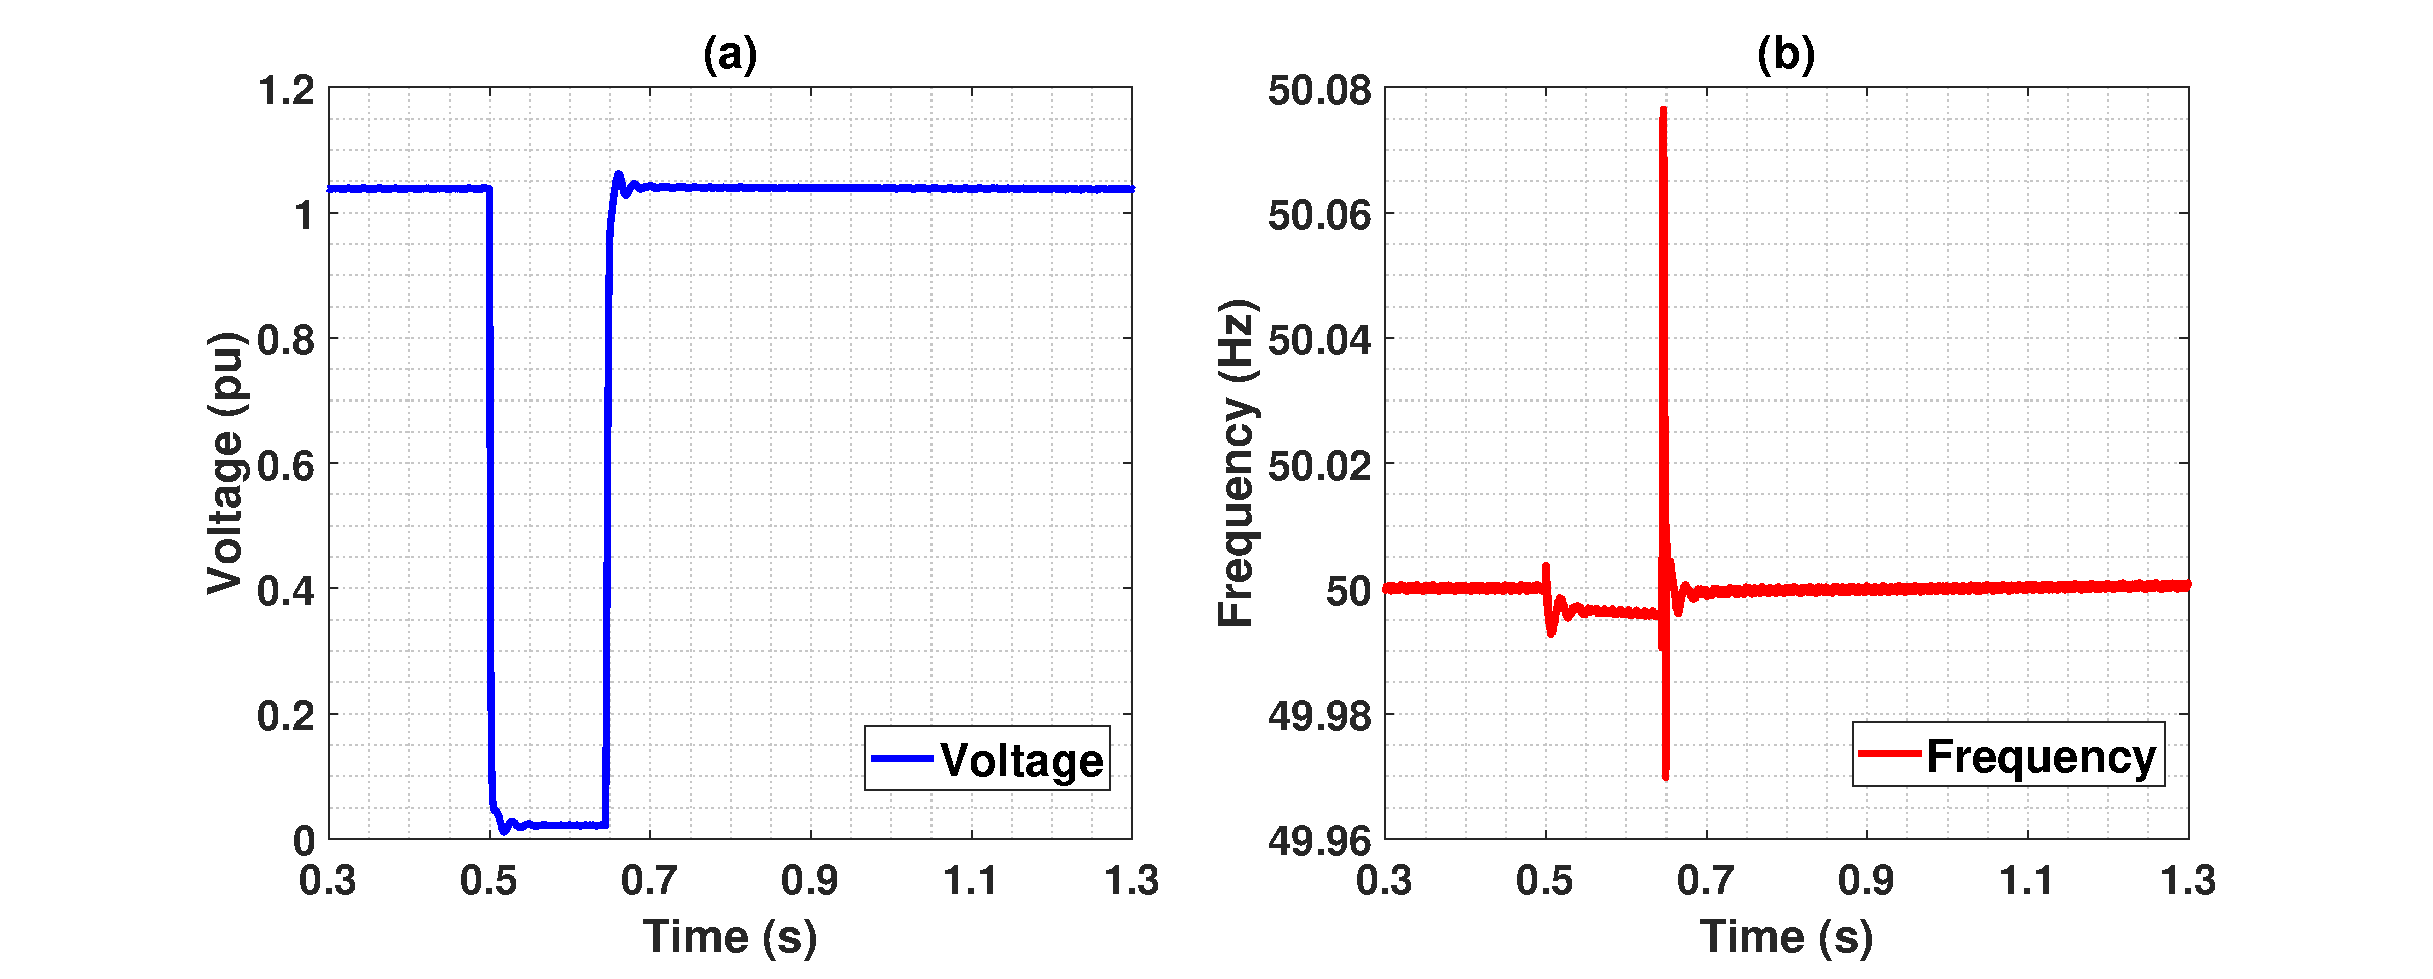
\includegraphics[height = 7cm,width = \textwidth]{Diagrams/Chapter_3/VACP_Freq_Final_3.eps}
    \caption{a) Voltage at PCC and b) Frequency response synthesised by PLL following a three phase fault in the middle of the cable}
    \label{fig:Vol_Freq_3phaseSC}
\end{figure}


\begin{figure}[H]
%\centering
%\hspace*{-0.1cm}
    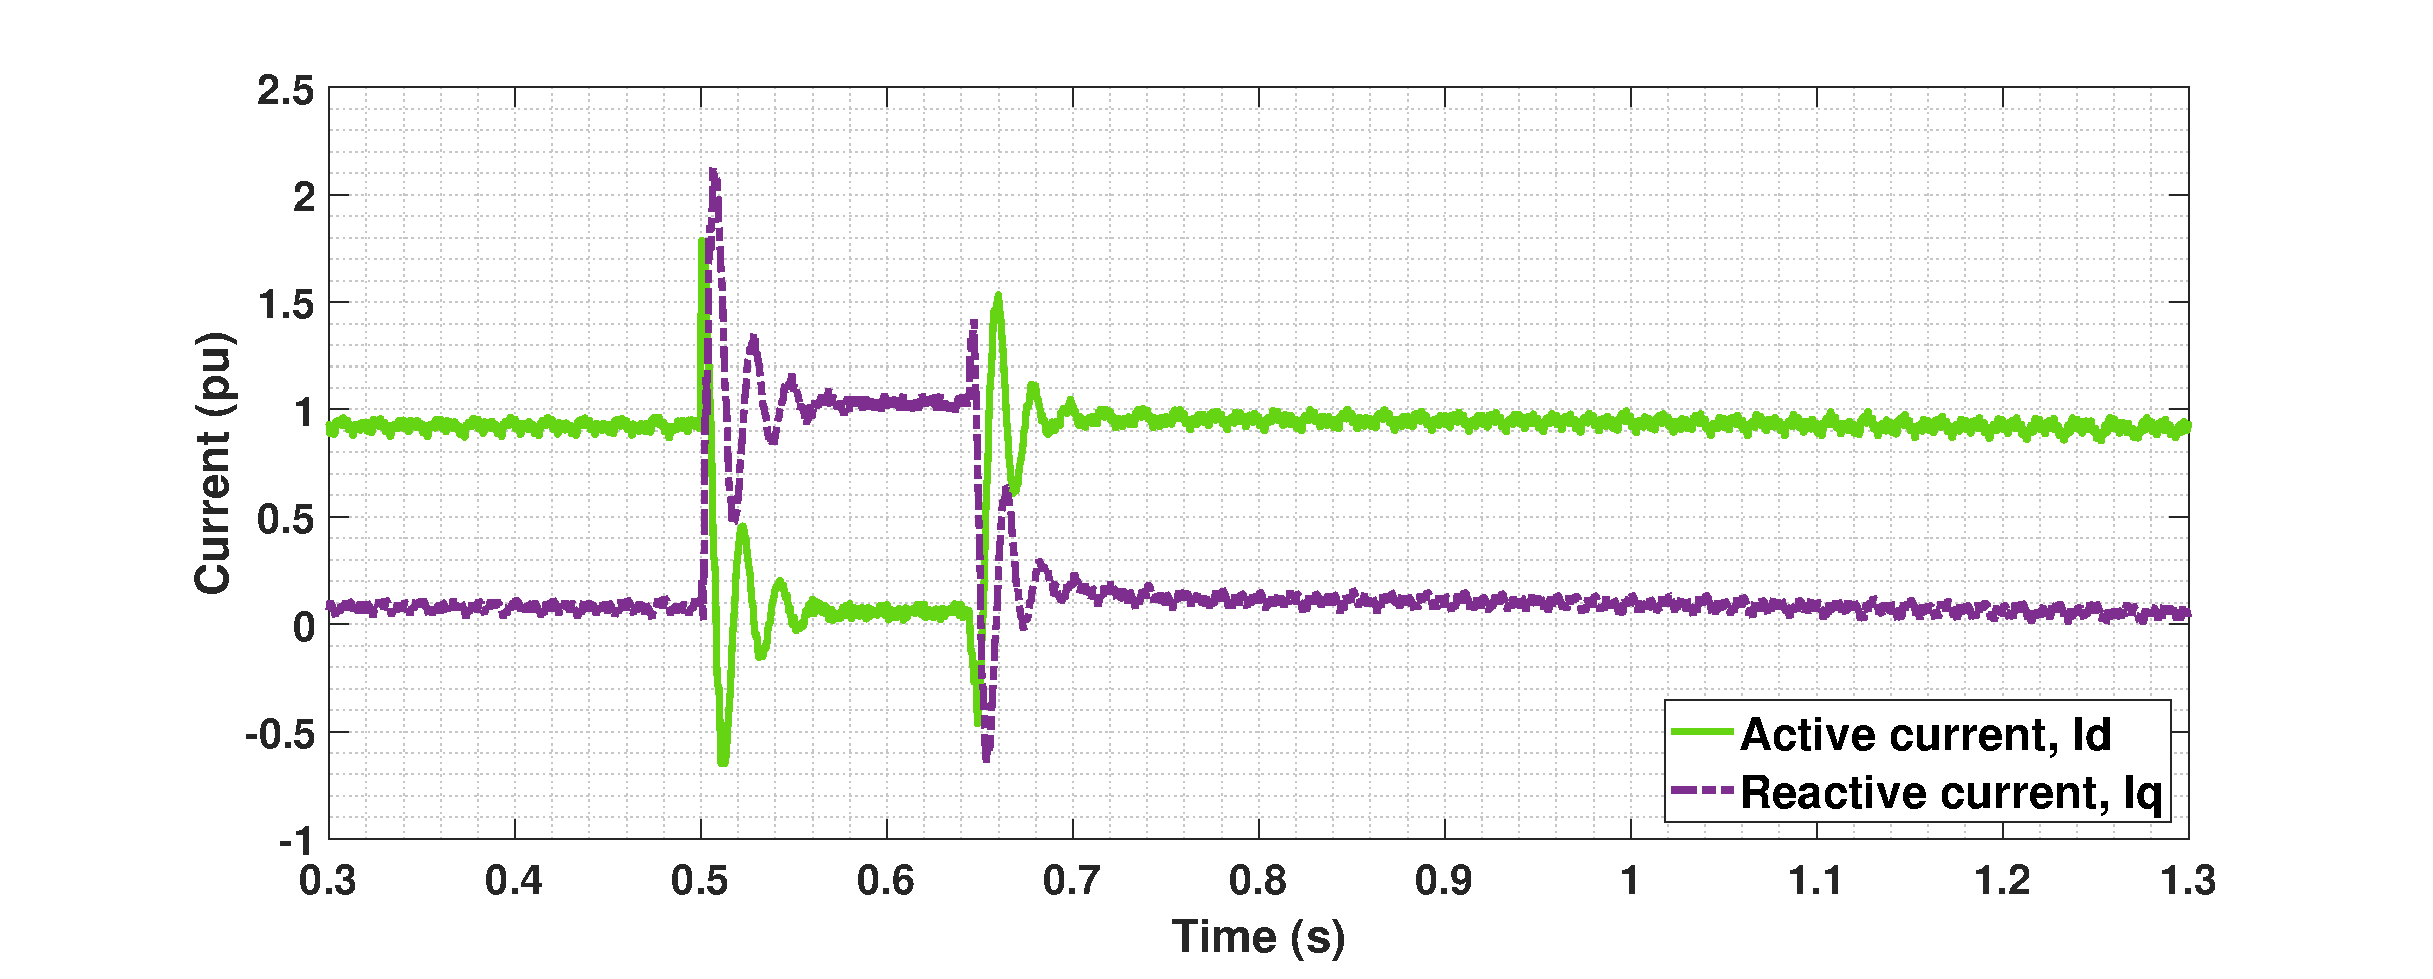
\includegraphics[height = 6.5cm,width = \textwidth]{Diagrams/Chapter_3/ID_IQ_Final_4.eps}
    \caption{Active and reactive currents flowing to the network for a three phase fault in the middle of the cable}
    \label{fig:ID_IQ_Final_3}
\end{figure}


\subsubsection{Parameter selection for Washout Filters}\label{para_selection_washout}
The damping during the transient process mentioned in Section \ref{DVC_theory} is ensured by the washout filters in the reactive power and active power control loops as seen in Figure \ref{fig:Reactive_Power_Control_Loop} and Figure \ref{fig:Active_Power_Control_Loop} respectively. The parameters for the washout filters need to be chosen wisely in order to ensure fast damping of transients. The output of the washout filter for various proportional gains for a step response is depicted in Figure \ref{fig:Washout_gain_output}. The proportional gain represents values to which the output of the washout filter changes when there is a change in the input. The time constant represents the rate of this change. It can be seen that the output of the washout filter changes proportionally to the gain value specified and comes back to the initial value after a specific time, depending on the time constant mentioned.


Effect of this property of the washout filter is observed in active and reactive currents of at the \gls{PCC} for a three-phase fault, as shown in Figure \ref{fig:ID_Washout_Comp} and \ref{fig:IQ_Washout_Comp} respectively. The proportional gain is set as 0.01, 0.03 and 0.05 for comparison keeping the time constant = 0.01 s for all the three cases. It is observed that faster damping can be achieved for higher proportional gains, as shown in Figure \ref{fig:ID_IQ_Washout_Comp}. It makes sense as the system would try to damp the transients to the maximum possible value in order to have minimum fluctuations and also to limit interactions with other controllers during this period. Thereby, it is worthy to conclude that choosing the right parameters for the washout filter is one among the key factors in this control approach.

\begin{figure}[H]
\centering
%\hspace*{-1cm}
    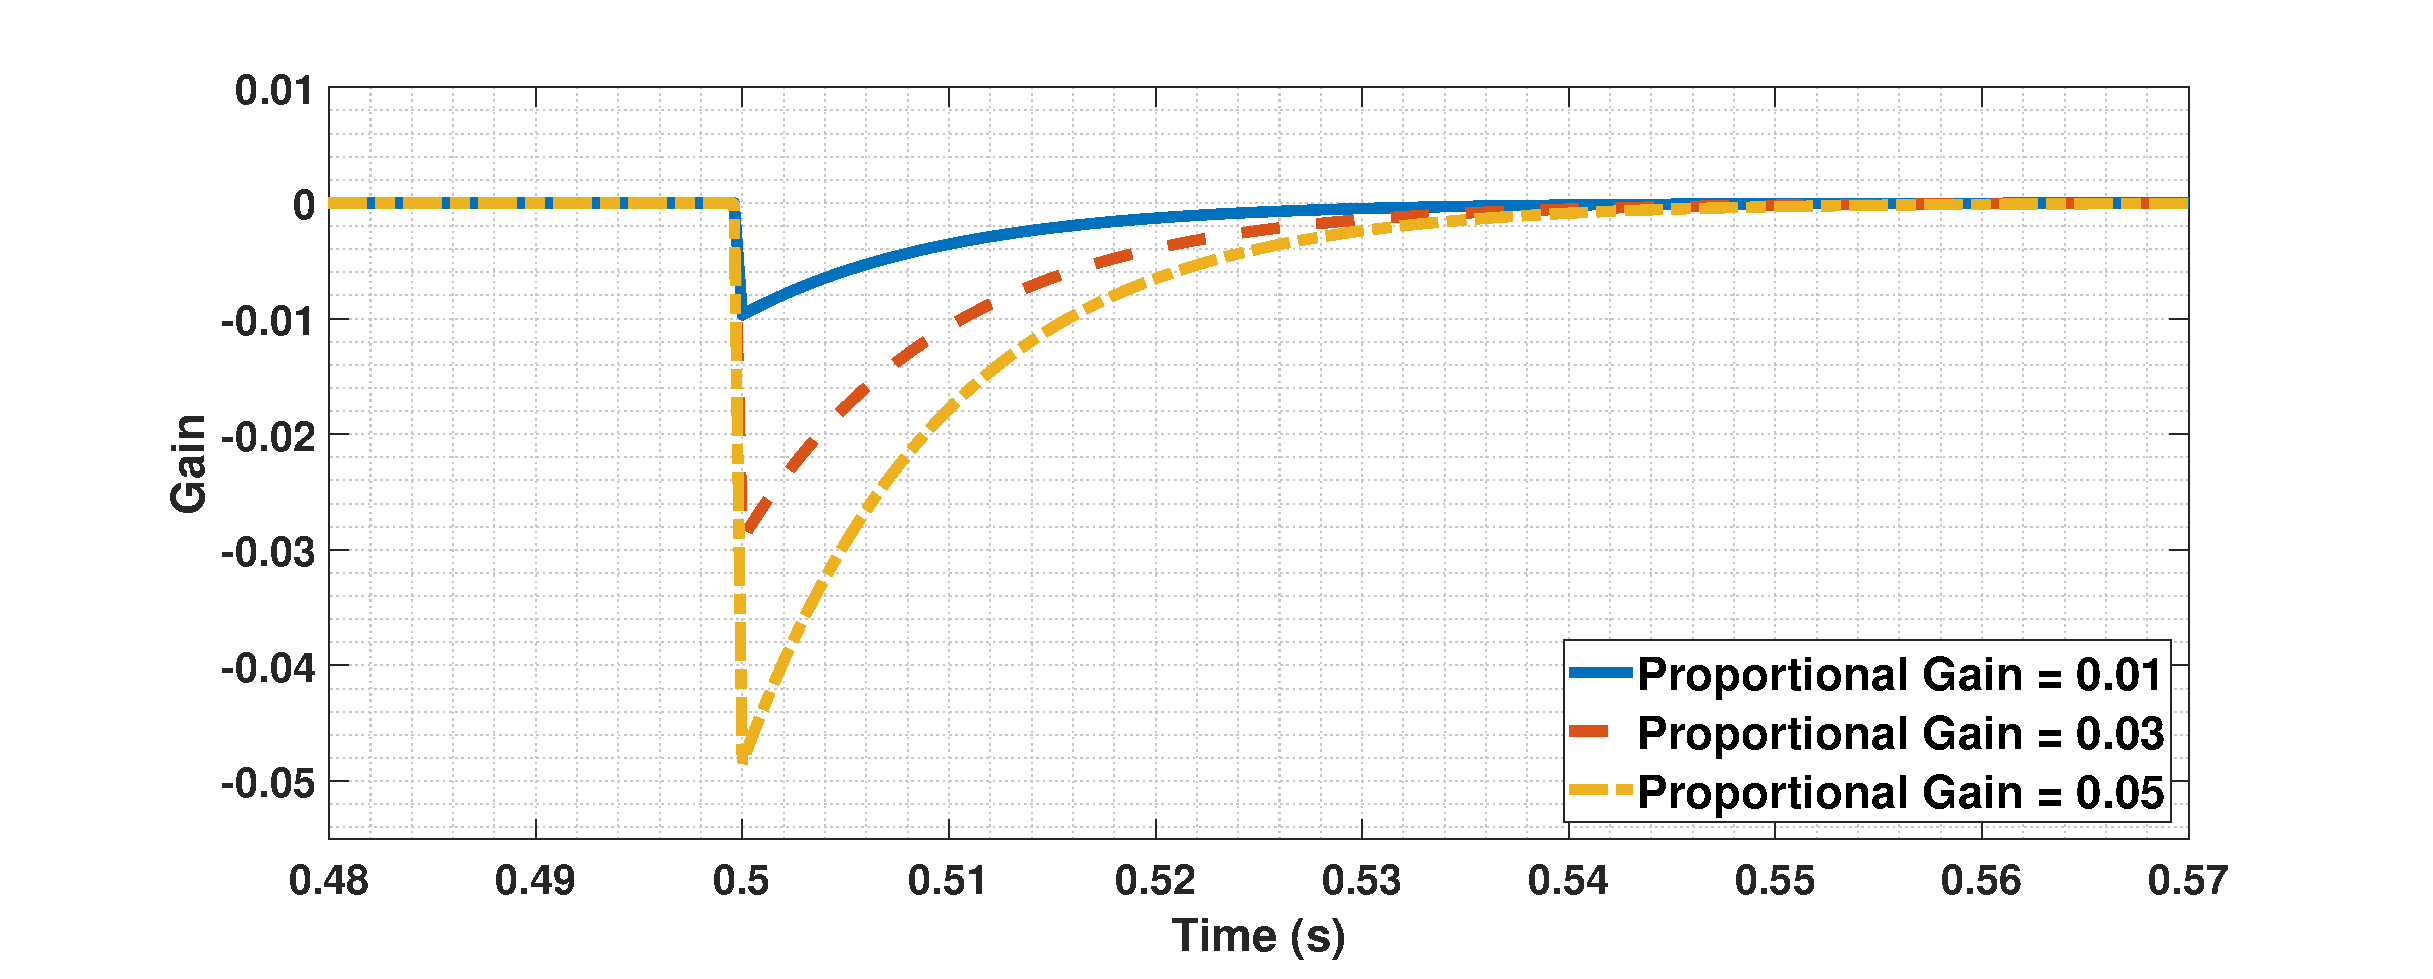
\includegraphics[height = 6cm,width = 14.5cm]{Diagrams/Chapter_3/Washout_gain_output_4.eps}
    \caption{Output of a washout filter for different proportional gains for a step response}
    \label{fig:Washout_gain_output}
\end{figure}

\begin{figure}[H]
%\centering
\begin{subfigure}{0.5\textwidth}
 % \centering
  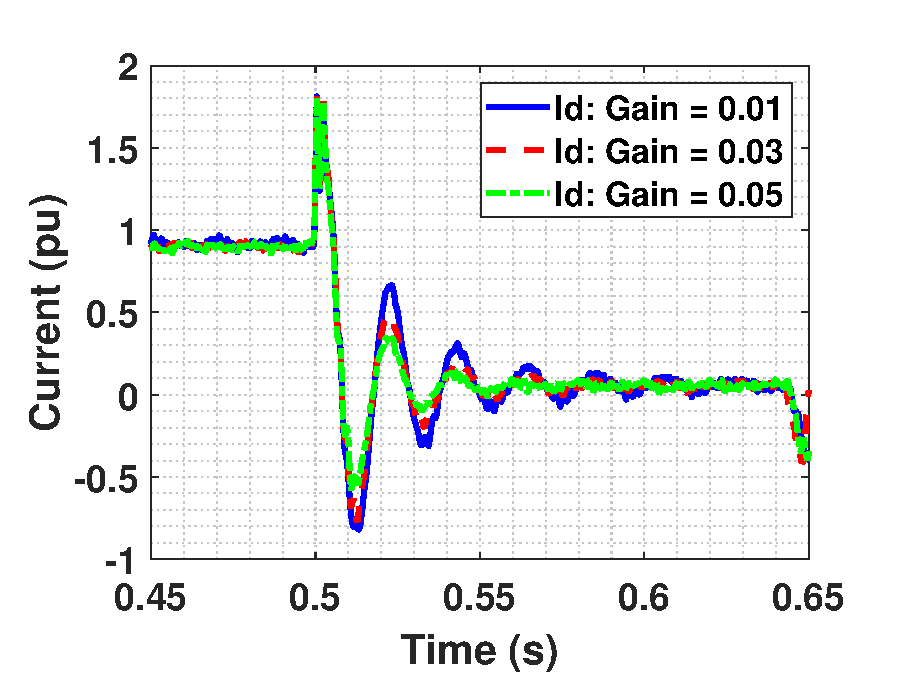
\includegraphics[height = 6.5cm,width = \textwidth]{Diagrams/Chapter_3/ID_Washout_Comp_4.eps}
  \caption{Current in d axis during three phase fault for gain 0.01, 0.03 and 0.05}
  \label{fig:ID_Washout_Comp}
\end{subfigure}%
\begin{subfigure}{0.5\textwidth}
  %\centering
  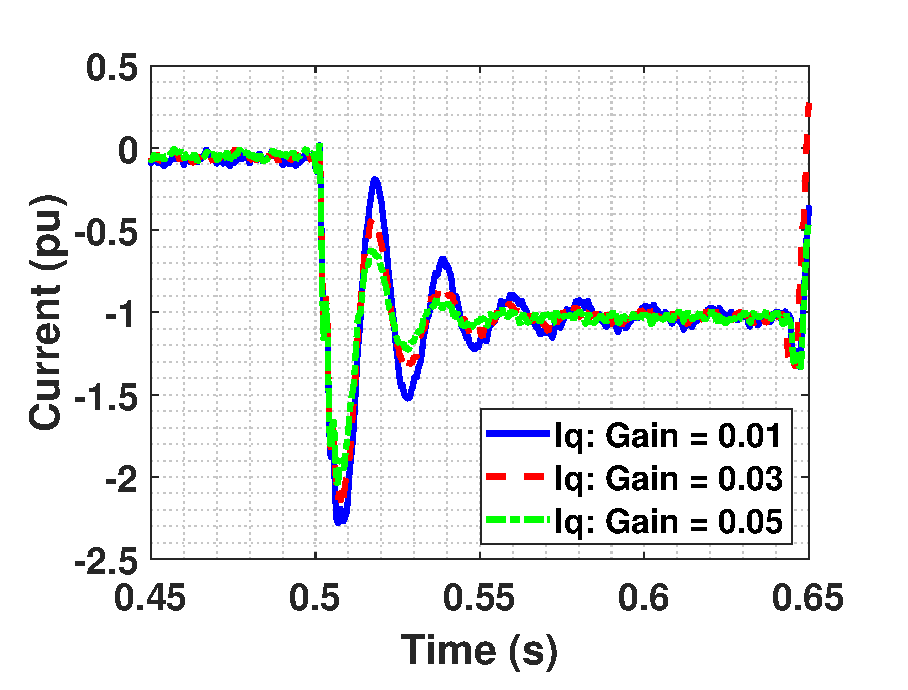
\includegraphics[height = 6.5cm,width = \textwidth]{Diagrams/Chapter_3/IQ_Washout_Comp_4.eps}
  \caption{Current in q axis during three phase fault for gain 0.01, 0.03 and 0.05}
  \label{fig:IQ_Washout_Comp}
\end{subfigure}
\caption{Currents in d and q axes during three-phase fault in the middle of the cable for different proportional gains of washout filters}
\label{fig:ID_IQ_Washout_Comp}
\end{figure}

\section{DIgSILENT PowerFactory Software}
PowerFactory is a software tool developed by DIgSILENT (Germany) that is used for RMS and EMT simulations. It has three integration characteristics, and they are functional integration, vertical integration and database integration. Functional integration explains that PowerFactory is a single executable program and vertical integration means that the models in the power system can exchange all of the analysis functions at one place. PowerFactory uses a Data Manager for database integration that allows all models to be stored under one project file. There are two libraries available in PowerFactory: Global and Project libraries. There are two subsections available within the Project library. They are \cite{powerfactory_tech}:
\begin{itemize}
    \item Equipment Type Library
    \item User Defined Models
\end{itemize}
PowerFactory also provides development of user-defined models using DIgSILENT Simulation Language (DSL). These features are utilized, and \gls{DVC} control is implemented in PowerFactory for a typical configuration of the offshore network in \cite{korai_dynamic_2019}. It is tested and proved to work \cite{korai_dynamic_2019}. The test results achieved in RSCAD in the previous section need to be compared with a similar 66 kV offshore network in PowerFactory to validate the control action. In this section, a 66 kV offshore network is built in PowerFactory with the \gls{DVC} model utilized from \cite{korai_dynamic_2019}. Differences in the models are notified, the voltage and current profiles are compared for a three-phase line to ground fault in the middle of the cable.

\section{Layout of the 66 kV HVAC test system in PowerFactory}

The 66 kV offshore network is modelled in PowerFactory as shown in Figure \ref{fig:WT1_Model_PFD_comp}. The network consists of the following components:

\begin{itemize}
    \item A simplified model of Full Scale Converter (FSC) based Type-4 \gls{WG} system consisting of the following elements:
    \begin{itemize}
        \item \gls{DC} circuit
        \item Grid Side Converter (\gls{GSC}) or Line Side Converter (\gls{LSC})
    \end{itemize}
    \item High Pass filter (\gls{HPF}) with series reactor
    \item \gls{OWF} transformer
    \item \gls{HVAC} cables  
    \item \gls{AC} equivalent source representing grid connection
\end{itemize}

\begin{figure}[H]
%\centering
%\hspace*{-1.2cm}
    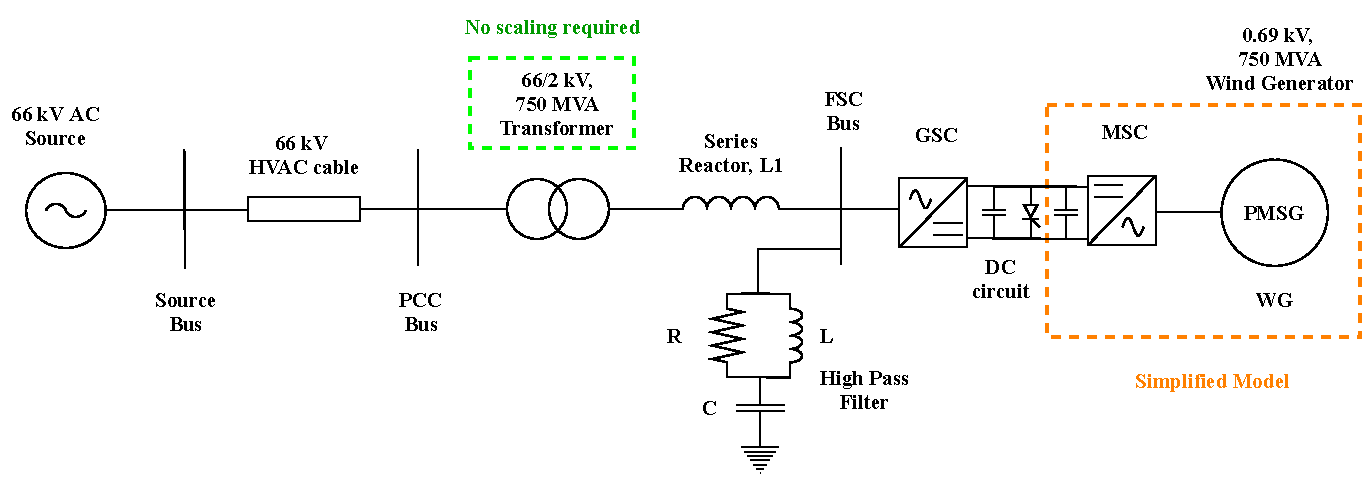
\includegraphics[height = 6cm,width = \textwidth]{Diagrams/Chapter_3/WT1_AC_PFD.pdf}
    \caption{Single line diagram of the 66 kV HVAC offshore test network in PowerFactory}
    \label{fig:WT1_Model_PFD_comp}
\end{figure}

\subsection{Simplified model of WG System}
The wind turbine and \gls{MSC} are simplified since they do not contribute to the dynamics of grid. \gls{LSC} is modelled in detail. A constant injection of active current is proposed from the \gls{MSC} to the \gls{DC} side \cite{korai_dynamic_2019}. Hence it is modelled as a \gls{DC} current source. The \gls{WG} unit is represented as a static generator model with 750 MVA nominal apparent power. It is made to operate with constant reactive power (Q) control in order to set the active and reactive power set points same as in RSCAD model. The active power flow is set to 700 MW, similar to the RSCAD model.

\subsubsection{DC Circuit}
The \gls{DC} voltage across the capacitor is set to 4 kV. The chopper activation control is provided when the \gls{DC} voltage crosses a minimum set value. 

\subsubsection{Line Side Converter (LSC)}
Unlike the RSCAD model, a two-level \gls{LSC} is utilized in this model. The \gls{PWM} is not used in this model, and the \gls{LSC} is modelled as a controlled voltage source. This is one among the major difference with the RSCAD model. The \gls{DVC} control for \gls{LSC} developed in \cite{korai_dynamic_2019} is provided in this model as explained in Section \ref{DVC_RSCAD}. The representation in PowerFactory is depicted in Appendix. [] 

\subsection{High Pass Filter (HPF) with Series Reactor}
The shunt filter available in the PowerFactory drawing toolbar is chosen. The values for R, L and C are chosen the same as mentioned in Section \ref{HPF_design}. A common impedance element available in the drawing tool is chosen for the series reactor and is connected at the output of \gls{LSC}, as shown in Figure \ref{fig:WT1_Model_PFD_comp}. The inductance value chosen is the same as the RSCAD model to have an equal impedance for both the models.  

\subsection{OWF Transformer}
A two winding transformer available in the equipment library folder of DIgSILENT library is used. The transformer is rated 66/2 kV, 750 MVA with a delta-wye configuration. The leakage inductance and resistance of the transformer are set the same as the RSCAD model.

\subsection{HVAC Cables}
The cables are rated at 66 kV same as the RSCAD model. The cable is modelled from the "Cables" section available in the equipment library in DIgSILENT library. The type of model is chosen to be the Pi model. %as shown in Figure \ref{fig:CableModel_PFD}. 
Pi model is utilized as it is easier to input the cable parameters in terms of RLC in both RSCAD and PowerFactory.

\subsection{External AC system}
The external \gls{AC} system in PowerFactory also represents an infinite grid. Similar to the model in RSCAD in Section \ref{ext_AC_source}, the infinite grid is modelled as a \gls{AC} voltage source available in the PowerFactory drawing toolbar. 

\section{Comparison of models in RSCAD and PowerFactory }
The major differences between the 66 kV \gls{HVAC} network built in RSCAD and PowerFactory are illustrated in Table. \ref{tab:Comp_RSCAD_PFD_Para}. 
\vspace{-1mm}
\begingroup
%\setlength{\tabcolsep}{10pt} % Default value: 6pt
\renewcommand{\arraystretch}{1.2} % Default value: 1
\begin{table}[H]
\centering
%\hspace*{-0.5cm}
\begin{tabular}{|c|c|c|}
\hline
\textbf{Parameters}            & \textbf{PowerFactory} & \textbf{RSCAD}            \\ \hline
Wind Generator         & Simplified (Constant power model)          & PMSG                      \\ \hline
Machine Side Converter control        & Not modelled          & Decoupled current control \\ \hline
Grid Side Converter & \multicolumn{1}{l|}{Controlled Voltage Source with no PWM} & {VSC with PWM} \\ \hline
Generated active power from WG & 700 MW                & 6 MW                      \\ \hline
Scaling factor at transformer  & Not applicable        & 117 (cf. Section. \ref{scaling_OWF})                      \\ \hline
\end{tabular}
\caption{Differences in models in PowerFactory and RSCAD}
\label{tab:Comp_RSCAD_PFD_Para}
\end{table}
\endgroup

\vspace{-6mm}
\paragraph{Representation of \gls{GSC}}: One of the differences in both models is the usage of average model representation of \gls{VSC} with \gls{PWM} in RSCAD for the \gls{GSC}, whereas a controlled voltage source model is utilized in the PowerFactory model.
\vspace{-3mm}
\paragraph{Scaling of power}: Another significant difference between the two models is that the components connected to the secondary side of the transformer are modelled for one \gls{WG} of 6 MW in RSCAD whereas it is directly modelled for 700 MW in PowerFactory. The scaling of power to 700 MW in RSCAD is done at the 66/2 kV \gls{OWF} transformer, as explained in Section \ref{scaling_OWF}. This helps in modelling and analysis in the real world in terms of single \gls{WG}.


\subsection{Selection of time step in RSCAD and PowerFactory}
Before the start of the simulation, a specific time step value suitable for both the RSCAD and PowerFactory models need to be set. As mentioned in Section \ref{OWF}, the ratio of large time step to small-time step needs to higher than 12 in RSCAD model if NovaCor processor is used. Hence a value of 50 $\mu$s was chosen for the large time step. The setting can be done by right-clicking on the Draft module and selecting "Circuit Options" in RSCAD. In PowerFactory, it can be edited in the "Step Size" option available in the "Calculation of initial conditions" tab, as shown in Figure \ref{fig:Stepsize_RSCAD_PFD}.  

\begin{figure}[H]
\centering
%\hspace*{-1.2cm}
\begin{subfigure}{.55\textwidth}
  \centering
  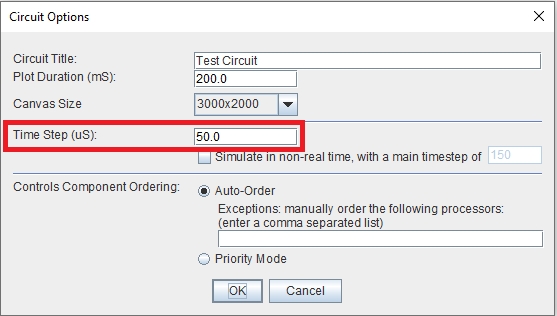
\includegraphics[height=4.5cm,width=7.5cm]{Diagrams/Chapter_3/Stepsize_RSCAD.PNG}
  \caption{Time step setting in RSCAD}
  \label{Stepsize_RSCAD}
\end{subfigure}%
\begin{subfigure}{.45\textwidth}
  \centering
  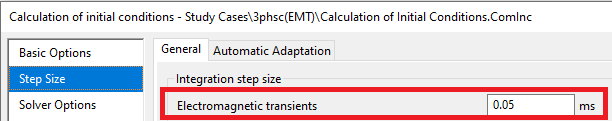
\includegraphics[height=1.6cm,width=7cm]{Diagrams/Chapter_3/Stepsize_PFD_Zoom.PNG}
  \caption{Time step setting in PowerFactory}
  \label{Stepsize_PFD_Zoom}
\end{subfigure}
\caption{Initialization of time step in RSCAD and PowerFactory}
\label{fig:Stepsize_RSCAD_PFD}
\end{figure}

\subsection{Event comparison in RSCAD and PowerFactory}
The 66 kV offshore network model in RSCAD and PowerFactory are compared for a three-phase short circuit in the middle of the cable. A fault is applied at 0.5 seconds with a clearing time of 140 ms. The resulting voltage and current waveforms are as shown in Figure \ref{fig:VACP_comp},  \ref{fig:ID_fullACSource} and \ref{fig:IQ_fullACSource} respectively. As can be observed in Figure \ref{fig:VACP_comp}, voltage drops and the generation is stopped during the fault period. The voltage profile is the same in RSCAD and PowerFactory models during the pre-fault, fault and post fault conditions as can be observed. The drop in voltage in both the graphs is the same due to equal impedance in both the models. 

\begin{figure}[H]
%\centering
%\hspace*{-1.2cm}
    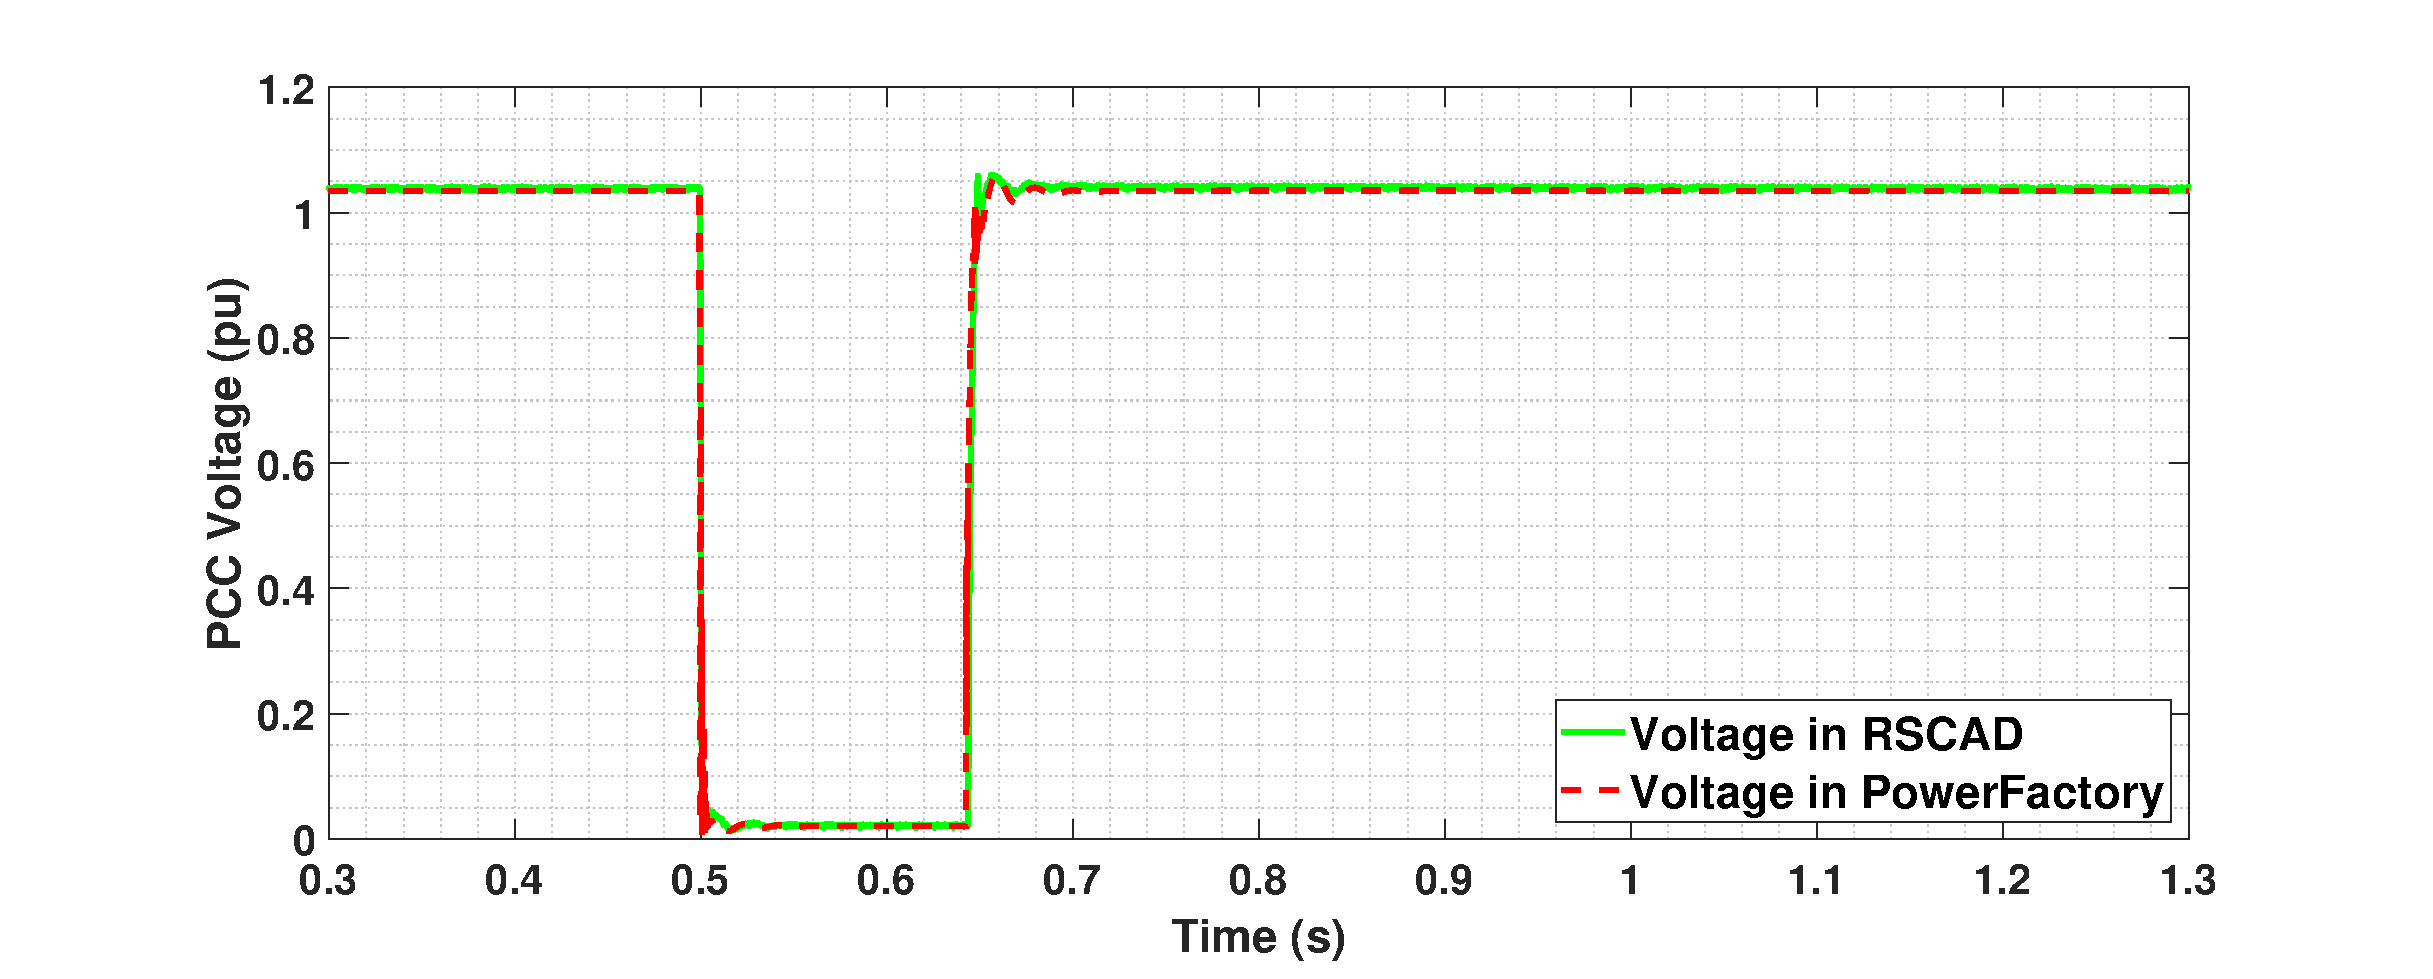
\includegraphics[height = 7cm,width = \textwidth]{Diagrams/Chapter_3/VACP_Comp_New_4.eps}
    \caption{Voltage measured at PCC for a three phase fault in the middle of the cable in RSCAD and PowerFactory}
    \label{fig:VACP_comp}
\end{figure}


Due to the unavoidable modelling difference of the software packages, the currents are measured at \gls{PCC} bus for the RSCAD model and at \gls{FSC} bus for the PowerFactory model. However, this does not affect the magnitude as the currents are measured in per unit. The currents in both the models have a similar profile, as summarized for the d-axis in Figure \ref{fig:ID_fullACSource} and q-axis in Figure \ref{fig:IQ_fullACSource}. The active and reactive currents generated by the \gls{WG} have the same set points in both the models during the steady state conditions confirming that the power flow in both the models is similar. The reactive power injection in RSCAD model during the time of fault is achieved similar to the PowerFactory model. The transients occurring during the time of fault can be damped by controlling the parameters of the washout filters, as seen in Section \ref{para_selection_washout}. The spike in the profiles is due to the dynamics of \gls{PLL} in both the software packages. Therefore, it can be concluded that the RSCAD model with the implemented \gls{DVC} provides accurate results similar to the benchmark PowerFactory model and can be used as a base model for reference as it provides a better representation of the real-world operation.  

\begin{comment}
\begin{figure}[H]
%\centering
%\hspace*{-1.2cm}
    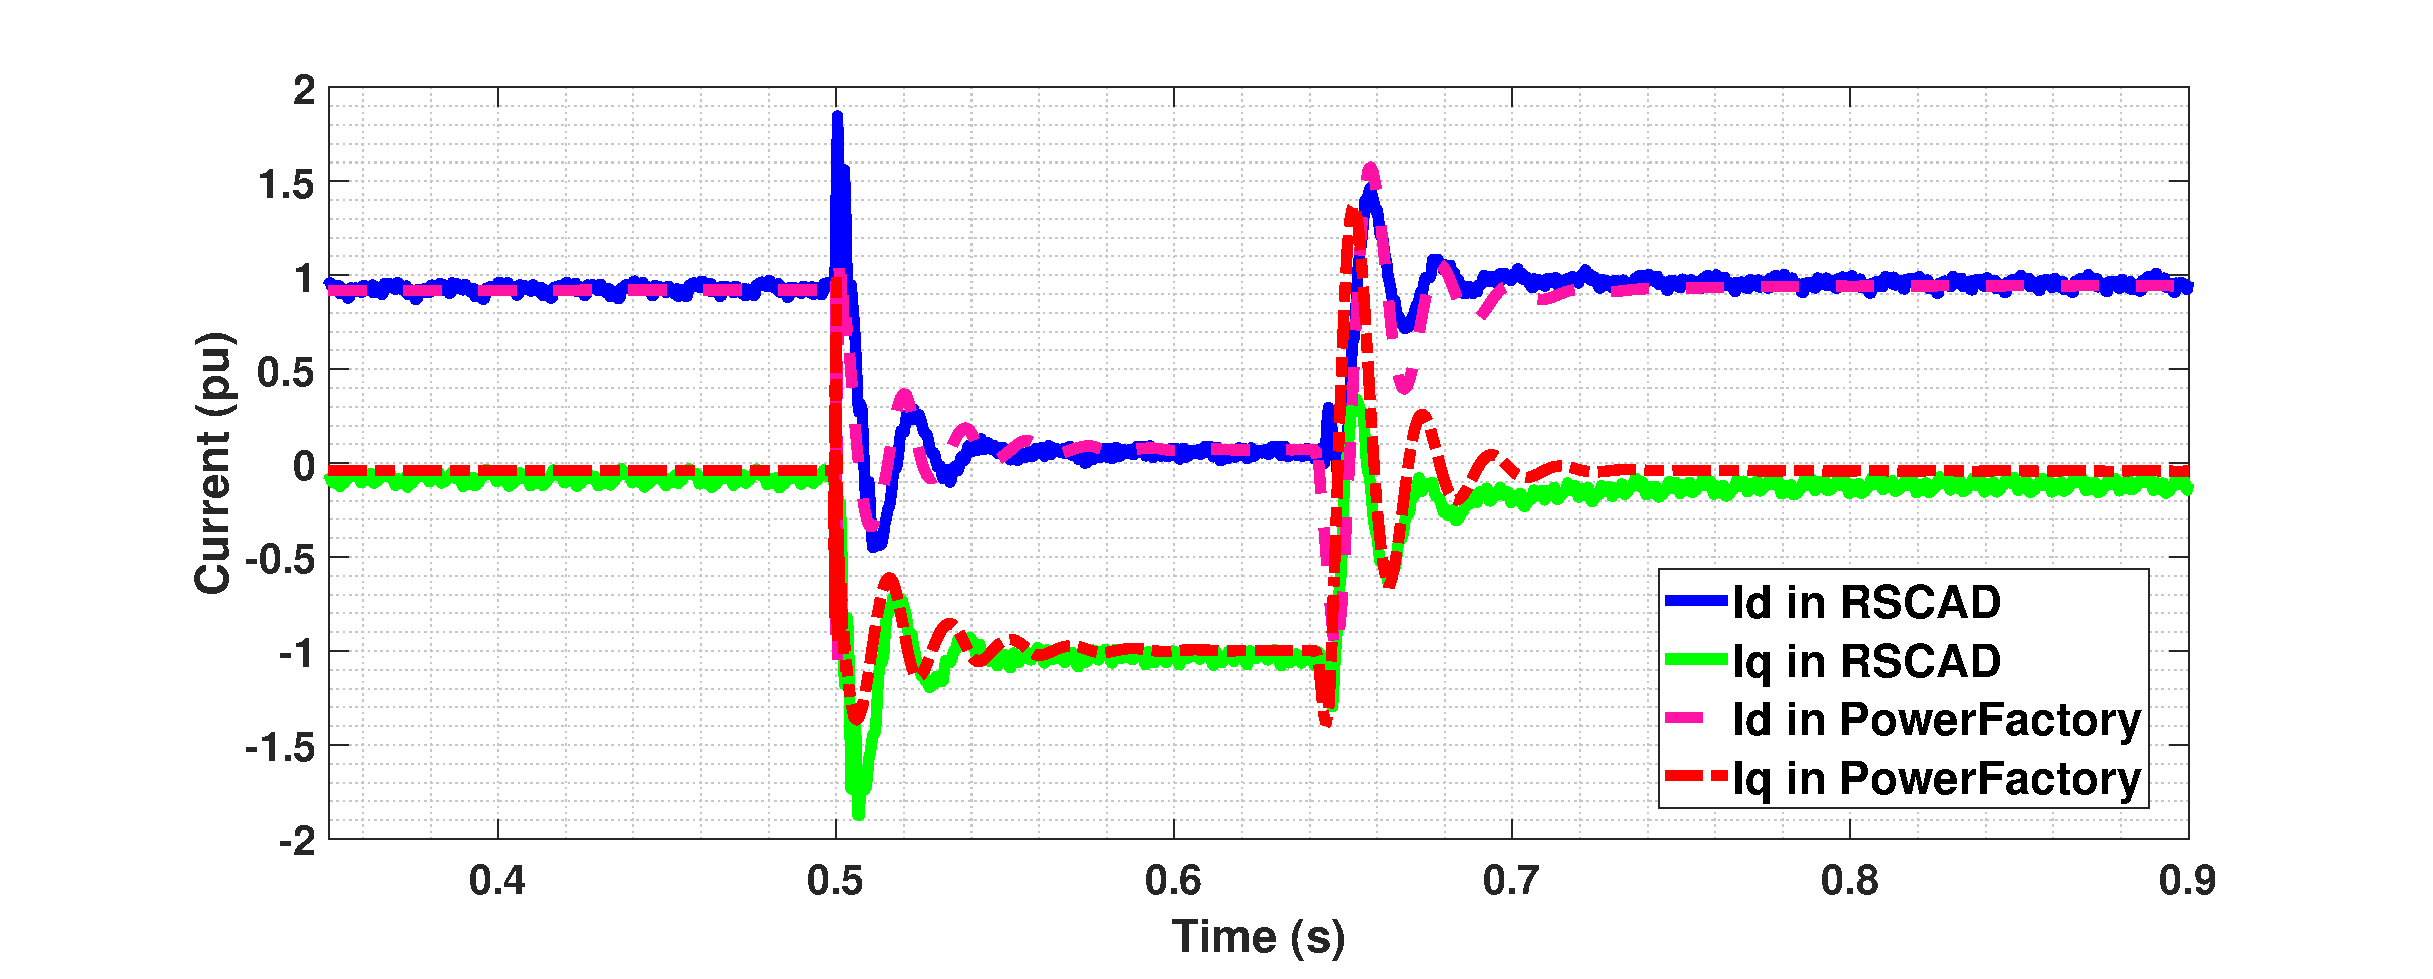
\includegraphics[height = 6cm,width = \textwidth]{Diagrams/Chapter_3/ID_IQ_Comp_New_3.eps}
    \caption{Active and reactive currents measured for a three phase fault in the middle of the cable in RSCAD and PowerFactory}
    \label{fig:ID_IQ_Comp}
\end{figure}
\end{comment}

\begin{figure}[H]
%\centering
%\hspace*{-0.1cm}
    \includegraphics[height = 7cm,width = \textwidth]{Diagrams/Chapter_3/ID_RSCAD_PFD_Comp.eps}
    \caption{Active currents flowing to the network for a three phase fault in the middle of the cable}
    \label{fig:ID_fullACSource}
\end{figure}
\vspace{-10mm}
\begin{figure}[H]
%\centering
%\hspace*{-0.1cm}
    \includegraphics[height = 7cm,width = \textwidth]{Diagrams/Chapter_3/IQ_RSCAD_PFD_Comp.eps}
    \caption{Reactive currents flowing to the network for a three phase fault in the middle of the cable}
    \label{fig:IQ_fullACSource}
\end{figure}
% \chapter{Modelling a Digital Twin of 2 GW, 66 kV HVAC Offshore Network with MMC-HVDC Transmission}\label{4}
This chapter details the development of a multi-gigawatt (focus of 2 GW), 66 kV \gls{HVAC} offshore network connected to two offshore converter stations. Like in Chapter \ref{3}, an average \gls{EMT} modelling depth is used (i.e. focus on the study of three-phase faults occurring in a balanced system), the model is developed and simulations are conducted in RSCAD. The model depicts the connection of four \gls{OWF}s through a 66 kV \gls{HVAC} offshore network contributing a total of 2 GW installed capacity. The power is transferred to the onshore system through \gls{MMC} based \gls{HVDC} links. The focus is to investigate the dynamic performance of such a system when subjected to severe disturbances (e.g. three-phase line to ground fault) in the \gls{AC} part of the network. The role of both \gls{DVC} in \gls{WG}s and voltage control in \gls{MMC} is examined in detail to understand the voltage performance and the power flow distribution based on simulations performed in RSCAD. %Firstly, the topology selected for the network is explained, and then the large scale network layout with all the components is detailed. The control structures utilized in the network is described in the final part of this chapter.

\section{Processors in RSCAD}\label{split_system}
The simulations in RSCAD can be run in either NovaCor or PB5 processor cards. NovaCor processor is used for this work as they have 2-3 times the simulation capacity of a completely loaded PB5 processor \cite{noauthor_novacor_nodate_1}. For an extensive power system network, NovaCor processor requires a part of the system to be placed in a separate subsystem. RSCAD allows provision for splitting of the network into subsystems if the network is large. The splitting is done by right-clicking on the main subsystem tag and choosing "Add Subsystem" as shown in Figure \ref{fig:subsystem_RSCAD} and this feature is utilized in this section. Tline modules are used to connect subsystems. The process is explained in Section \ref{Tline_cable_RSCAD} in detail.

There are two NovaCor processors available at TU Delft and they are equipped with four cores each. These cores are utilized to solve the overall network solution, auxiliary components (such as transformers, cables, generators etc.) and the controls present in the simulation. Assignment of cores for solving various components of the network is an important step that needs to be considered while modelling, as they depict the total load that is distributed over the available cores. The process is detailed in Section \ref{Aggregated_OWF_large_scale}. 

\begin{figure}[H]
\centering
%\hspace*{-1.2cm}
    \includegraphics[height = 2cm,width = 3.5cm]{Diagrams/Chapter_3/Subsystem.PNG}
    \caption{Adding subsystems in RSCAD}
    \label{fig:subsystem_RSCAD}
\end{figure}


\section{Defining the Layout for the 2 GW Offshore Network}
The initial aspect that needs to be considered for a offshore network is the topology of the network. The popularity of \gls{MMC} due to its improved controllability and superior system performances has led way for the increasing demand for \gls{MMC}-\gls{HVDC} transmission for integration of long distance \gls{OWF}s. For the connection of new \gls{OWF}s in the vicinity of the already existing ones, parallel operation of \gls{MMC}-\gls{HVDC} transmission systems can be expected in the near future with multiple connections to the onshore system. Such type of schemes increase the interest in hybrid systems with the hub-and-spoke principle proposed by ABB \cite{abb_hvdc_2018} and represented in Figure \ref{fig:ABB_Hub_Spoke_3}. The layout in Figure \ref{fig:ABB_Hub_Spoke_3}a) depicts the connection of \gls{OWF}s to a offshore converter station which in turn transfers power to the onshore system through multi-terminal \gls{HVDC} connections. However, in such a layout, the idea of scaling of offshore wind power is limited to the installed capacity of the \gls{MMC} unit. Another layout involves the \gls{OWF}s connected through \gls{AC} links to a back-to-back \gls{HVDC} converter station as shown in Figure \ref{fig:ABB_Hub_Spoke_3}b). Long distance \gls{HVAC} transmission is required in this case, for the transfer of power from \gls{OWF}s to the onshore network and hence contribute to high losses in the network when compared to \gls{HVDC} transmission for larger distances. Figure \ref{fig:ABB_Hub_Spoke_3}c) represents the connection of multiple \gls{OWF}s to the offshore converter station, and power is transferred to the onshore system through multiple \gls{HVDC} links. Such a layout provides contingency in the network by supplying offshore wind power to at least one onshore system if one of the \gls{HVDC} links gets disconnected \cite{lescale2012parallelling}. A stage-wise construction of such a \gls{HVDC} project is easier to be achieved by the developers as well \cite{cigre_B455}.

A specific configuration for a 2 GW offshore network is currently non-existent and this chapter tries to fill in such a research gap. The idea in this chapter is to expand the single \gls{OWF} model network in Figure \ref{fig:WT1_Model_RSCAD} for a 2 GW offshore wind power network. This could be made possible by connecting four such \gls{OWF} models in parallel with each generating 500 MW of power. The reason for choosing four \gls{OWF}s is to have a symmetrical layout and to test the ability of RSCAD to perform simulations of such a configuration. Correspondingly, a 2 GW offshore converter station capacity is required to transfer this generated amount of power to the onshore system. However, currently deployed (state-of-the-art) \gls{MMC}-\gls{HVDC} transmission, has a maximum rated capacity of 1.2 GW \cite{peralta2012detailed}. Hence, with the available technology, two \gls{MMC} offshore stations of 1 GW each will be required for 2 GW power transmission. Taking the aforementioned factors into account, a modified layout of Figure \ref{fig:ABB_Hub_Spoke_3}c) is developed for this work. 

\begin{figure}[H]
\centering
%\hspace*{-1.2cm}
    \includegraphics[height = 12cm,width = \textwidth]{Diagrams/Chapter_4/ABB_Hub_Spoke_3.png}
    \caption{a) Hub-and-spoke with multi-terminal HVDC system, b) Hub-and-spoke with AC links and HVDC back-to-back station and c) Hub-and-spoke with multiple HVDC links \cite{abb_hvdc_2018}}
    \label{fig:ABB_Hub_Spoke_3}
\end{figure}

\subsection{Scaling of Single OWF Model for 2 GW Offshore Network}\label{scaling_2GW}

The layout of 2 GW network is built by resorting to scaling of the aggregated \gls{OWF} model in Section \ref{OWF} of Chapter \ref{3}. A modular topology is considered to achieve the capacity of 2 GW. 

\begin{itemize}
    \item The aggregated \gls{OWF} model in Section \ref{OWF} provides a generation of 700 MW. The first step involves reducing this generation to approximately 500 MW as the layout is planned for four \gls{OWF}s. This is achieved by reducing the number of parallel \gls{WG} units from 116 (116 x 6MW = 696 MW) to 83 (83 x 6MW = 498 MW) which is done by changing the scaling factor explained in Section \ref{scaling_OWF}. Now the \gls{OWF} generates nearly 500 MW of active power, as shown in Figure \ref{fig:Steps_for_Scaling}a).
    \item The second step involves connection of two \gls{OWF}s in parallel to the external \gls{AC} system in a modular approach. This allows for generation of 1 GW of power as depicted in Figure \ref{fig:Steps_for_Scaling}b). All the control structures incorporated in \gls{OWF}-1 are replicated for \gls{OWF}-2.
    \item In the third step, the external \gls{AC} system is replaced by an offshore converter station consisting of the average \gls{EMT} model of \gls{MMC} (\gls{MMC}-1) and the interface transformer (IT-1) available in the CIGRE B4 DC Grid Test System \cite{vrana2013cigre}. The same is depicted in Figure \ref{fig:Steps_for_Scaling}c). As the final layout network would be extensive it is required to split the network into subsystems, as mentioned in Section  \ref{split_system}. The splitting into two subsystems is performed in this step. The offshore converter station is modelled in subsystem-1 and the \gls{OWF}s are modelled in subsystem-2. \gls{MMC}-1 is designed to operate in V/F control (or grid forming control) which is explained at the end of this chapter.
    \item The final step involves parallel connection of two more \gls{OWF} models (\gls{OWF}-3 and \gls{OWF}-4) in a modular approach generating 500 MW each. Additionally, another offshore converter station consisting of a similar average \gls{EMT} model of \gls{MMC} (\gls{MMC}-2) and two interface transformers (IT-2a and IT-2b), is connected in parallel to the previous converter station. The need for two interface transformers in \gls{MMC}-2 bus is explained at the end of this chapter. Therefore, the final layout shown in Figure \ref{fig:WT4_MMC2} represents a total of 2 GW offshore wind power transmission.
\end{itemize}


% Therefore by using the average \gls{EMT} model of an \gls{MMC} described in utilizing the available models for \gls{MMC}s, to enhance and understand the operation of Type-4 \gls{WG}s in parallel operation and their coordination with \gls{MMC}s, an \gls{AC} collector grid topology with parallel connection of two point-to-point \gls{HVDC} transmission system is implemented for this thesis work in RSCAD. 



%The development of the layout involves major three steps:

%The layout of the model is developed by connecting four \gls{OWF} 


\begin{figure}[H]
%\centering
%\hspace*{-1.2cm}
    \includegraphics[height = 21cm,width = \textwidth]{Diagrams/Chapter_4/Steps_for_Scaling.pdf}
    \caption{a) OWF-1 connected to external AC system, b) OWF-1 and OWF-2 connected in parallel to external AC system c) OWF-1 and OWF-2 connected in parallel to MMC-1}
    \label{fig:Steps_for_Scaling}
\end{figure}

\begin{figure}[H]
%\centering
%\hspace*{-1.5cm}
    \includegraphics[height = 12cm,width = \textwidth]{Diagrams/Chapter_4/WT4_MMC2_new.pdf}
    \caption{Single line diagram of 2 GW, 66 kV HVAC offshore network connected to 2 x 1 GW HVDC links with offshore converter stations in RSCAD}
    \label{fig:WT4_MMC2}
\end{figure}

\section{Layout of 2 GW, 66 kV HVAC Offshore Network in RSCAD}

The components in the 2 GW, 66 kV \gls{HVAC} network is detailed in this section. The single line diagram of the network is depicted in Figure \ref{fig:WT4_MMC2} and the major components of the network include :
\begin{itemize}
    \item Four aggregated \gls{OWF}s, each with 500 MW installed capacity represented by the following components:
    \begin{itemize}
        \item A single Wind Generation System with 
    \begin{itemize}
        \item Permanent Magnet Synchronous Generator (\gls{PMSG})
        \item Machine Side Converter (\gls{MSC})
        \item \gls{DC} circuit
        \item Grid Side Converter (\gls{GSC}) 
    \end{itemize}
        \item High Pass filter (\gls{HPF}) with series reactor
        \item \gls{OWF} transformer
    \end{itemize}
    \item Four \gls{HVAC} cables  
    \item Three interface transformers
    \item Two \gls{MMC}s
    \item Two pairs of \gls{HVDC} cables
\end{itemize}

\subsection{Aggregated OWF}\label{Aggregated_OWF_large_scale}
As mentioned in Section \ref{scaling_2GW}, the 2 GW offshore wind power is split into four \gls{OWF}s with 500 MW rated capacity each. Currently, the largest offshore \gls{WG} developed by GE Renewable Energy has a rating of 12 MW \cite{noauthor_worlds_2020}. However, the standard model available for a Type-4 \gls{WG} in RSCAD is rated 6 MW. Hence, to represent a 500 MW \gls{OWF}, 83 \gls{WG}s are required. All the \gls{OWF}s are at a distance of 30 kms from the \gls{MMC} bus. 


The average model of Type-4 \gls{WG} available in RSCAD is used for this work as well. The aggregated \gls{OWF} model represented in small time step environment described in Section \ref{OWF} is used here for all the four \gls{OWF}s. As the entire network is extensive, it is split into two subsystems in RSCAD as shown in Figure \ref{fig:WT4_MMC2} by employing the technique explained in Section \ref{split_system}. The four \gls{OWF}s are modelled in subsystem-2 and the rest of the system is modelled in subsystem-1. Each subsystem requires one rack for operation and hence two NovaCor racks are used for the network simulation. It is also possible to simulate the network with PB5 processor. However, this requires a total of three subsystems since PB5 racks allow only small network solutions to be solved in one rack \cite{noauthor_pb5_nodate_1}. Therefore, two \gls{OWF}s are to be modelled in subsystem-3, other two \gls{OWF}s in subsystem-2 and the rest of the network in subsystem-1. Henceforth, the simulations are considered only in NovaCor processor for this study.  


Since there need to be four different small time step blocks representing four \gls{OWF}s, each block needs to be set with different step sizes so as to avoid conflict during initialization. These step sizes are only used for initialization and the actual step sizes can be viewed in the "Map File" as mentioned in Section \ref{OWF}. Moreover, if the time steps are not initialized properly, it could lead to the occurrence of a time step overflow error during the simulation in the Runtime module. 


Another important parameter to be considered here is the assignment of the cores for the small time step blocks. As mentioned in Section \ref{split_system}, cores are responsible for solving the entire network solution. NovaCor processor in TU Delft is configured with four cores and each component used in the network can be assigned to specific cores (1 to 4 in number). Since there are six small time step blocks (\gls{OWF}-1, 2, 3 and 4; \gls{MMC}-1 and \gls{MMC}-2) in total, the cores need to be manually assigned to each block to allocate the load on each processor within their capacity. The core allocation of the small time step blocks representing \gls{OWF}s for this network is chosen as shown in Table \ref{tab:Core_assignment_sub2}.  

   

\begin{table}[H]
\centering
\begin{tabular}{|c|c|}
\hline
\textbf{Small time step block} & \textbf{Core assignment} \\ \hline
OWF-1                          & 4                        \\ \hline
OWF-2                          & 1                        \\ \hline
OWF-3                          & 3                        \\ \hline
OWF-4                          & 1                        \\ \hline
\end{tabular}
\caption{Core assignment of OWF models in subsystem-2}
\label{tab:Core_assignment_sub2}
\end{table}

\subsection{HVAC Cables}\label{Tline_cable_RSCAD}
The \gls{HVAC} cables transfer power from the \gls{OWF}s to the offshore converter stations. Hence, four sets of \gls{HVAC} cables are required to transfer power from four \gls{OWF}s. The cables are rated at 66 kV and are 30 kms of length. In the network layout represented in RSCAD, as shown in Figure \ref{fig:WT4_MMC2}, the \gls{HVAC} cables connect the \gls{OWF}s in subsystem-1 with the \gls{MMC} bus in subsystem-2. To provide such a connection between components placed in different subsystems in RSCAD, a feature called Tline module is available in the RSCAD modules section (denoted by a red box in Figure \ref{fig:TlineModule_mark}). This module is similar to the Cable module explained in Section \ref{HVAC_cable_RSCAD}. However, Cable module only allows connection between components in the same subsystem. The Tline module can be modelled as overhead transmission line or cable. Since an offshore network model is considered in this work, the Tline model represents a subsea cable model. 

The cables are modelled as Bergeron models with RLC data parameters. Bergeron model is chosen to test the working of the network using travelling wave model. Moreover, as the 2 GW offshore network is developed from the single \gls{OWF} model in Section \ref{OWF}, the same RLC cable parameters used in Section \ref{HVAC_cable_RSCAD} are used in the Tline module for all the four sets of cables. 
 
 \begin{figure}[H]
\centering
%\hspace*{-1.2cm}
    \includegraphics[height = 4.5cm,width = 7.5cm]{Diagrams/Chapter_4/Tline_module_Final.png}
    \caption{Tline module in RSCAD}
    \label{fig:TlineModule_mark}
\end{figure}
 
 In the Draft module, the cable model is added in the circuit using the unified Tline model shown in Figure \ref{fig:Tline_calculationbox_RSCAD} available in RSCAD power system library. The unified model consists of the following components: 
%\setlist{nolistsep}
    \begin{itemize}[noitemsep]
    \item Calculation Block
    \item Sending End Terminal
    \item Receiving End Terminal
\end{itemize}

The detailed representation of the cable parameters in Tline module, and the representation of the cable model using the calculation block, sending end terminal and receiving end terminals in the Draft module is shown in Appendix \ref{config_Tline}.

\begin{figure}[H]
  \centering
  % include first image
  \includegraphics[height = 5cm,width = 8cm]{Diagrams/Chapter_4/TlineParaBlock.PNG}  
  \caption{Tline configuration in Draft module in RSCAD}
  \label{fig:Tline_calculationbox_RSCAD}
\end{figure}

As the significant goal is to estimate the dynamic performance of the network under severe disturbances, a three-phase short circuit event in the middle of \gls{HVAC} cable-1 is chosen. To perform a short circuit event in the middle of a 30 km long \gls{HVAC} cable in RSCAD, two cable models of 15 kms length are modelled and connected in series, and the three-phase fault logic available in RSCAD library is modelled in the middle of the two cables as shown in Figure \ref{fig:Subsystem_Trial}. It must be noted that each cable model contain one set of sending and receiving end terminals. In order to connect two subsystems, the sending end terminal from the \gls{OWF} is placed in subsystem-2, and its receiving end is placed in subsystem-1. %The representation of one \gls{OWF} and one set of \gls{HVAC} cable in two subsystems in RSCAD is shown in Figure  \ref{fig:Subsystem_Trial}. All \gls{OWF}s placed in subsystem 2 are connected to the rest of the system in system 1 using \gls{HVAC} cables in a similar fashion.

\begin{figure}[H]
\centering
%\hspace*{-0.8cm}
    \includegraphics[height = 5.4cm,width = 17cm]{Diagrams/Chapter_4/subsystem_fault_mark.pdf}
    \caption{Representation of three-phase line to ground fault in the middle of HVAC cable-1 in RSCAD}
    \label{fig:Subsystem_Trial}
\end{figure}

\subsection{Offshore Converter Stations}
The offshore converter stations convert the \gls{HVAC} offshore wind power to \gls{HVDC} to transfer the power to the onshore system through \gls{HVDC} links.  %There are two offshore \gls{MMC} stations utilized in this network. 
The existing available \gls{HVDC} links in the industry have a rated capacity of 1.4 GW. Examples for such projects are the NordLink cable connecting Norway and Denmark, NSN Link connecting Norway and the United Kingdom \cite{ryndzionek_evolution_2020}. Moreover, the standard \gls{EMT} models for \gls{MMC}s available in CIGRE B4 DC Grid Test System \cite{vrana2013cigre} have a rated capacity of 1.2 GW. Therefore, with the currently available technology, two offshore converter stations are required for the transfer of 2 GW offshore wind power. From the description of \gls{MMC} explained in Section \ref{HVDC_trans_theory}, it can be understood that \gls{MMC}s also involve \gls{PE} components. Hence, similar to the \gls{OWF} model, the average \gls{EMT} models of \gls{MMC}s are represented in the small time step blocks in RSCAD to accurately represent fast switching events. The average \gls{EMT} models available in RSCAD consists of the \gls{MMC} and interface transformer modelled in the small time step environment representing the offshore converter station. For this work, two small time step blocks are required for the representation of two offshore converter stations. Both the blocks are placed in subsystem-1. These two blocks must be initialized with different time step to avoid conflict during initialization, and thereby avoiding the time step overflow error during the start of simulation in the Runtime module. To evenly distribute the load on four cores, considering the core allocation for \gls{OWF}s in Table \ref{tab:Core_assignment_sub2}, the cores for \gls{MMC}s are allocated as shown in Table \ref{tab:Core_assignment_sub1}. The offshore converter station-1 consists of the interface transformer (IT-1) and \gls{MMC}-1 whereas offshore converter station-2 consists of the interface transformers (IT-2a, IT-2b) and \gls{MMC}-2. 
%RSCAD also allows modelling in substep environment that can have a time step as small as 500 ns if the circuit is simple.    

\begin{table}[H]
\centering
\begin{tabular}{|c|c|}
\hline
\textbf{Small time step block} & \textbf{Core assignment} \\ \hline
MMC-1                          & 3                        \\ \hline
MMC-2                          & 2                        \\ \hline

\end{tabular}
\caption{Core assignment of MMC models in subsystem-1}
\label{tab:Core_assignment_sub1}
\end{table}


\subsubsection{Interface Transformers}
The interface transformers (also termed as converter transformers) are connected to the \gls{AC} side of the \gls{MMC}s and are depicted as IT-1 for offshore converter station-1 and IT-2a and IT-2b for offshore converter station-2 as shown in Figure \ref{fig:WT4_MMC2}. As explained in \cite{cigre2005b4}, these transformers entail the following main implications:
\begin{itemize}
    \item Providing a reactance between the offshore grid and the \gls{MMC}.
    \item Preventing the flow of zero sequence currents between the offshore grid and the \gls{MMC}.
\end{itemize} 

 %The three-phase three identical single-phase transformer \gls{VSC} interface model available in the RSCAD library shown in Figure \ref{fig:InterfaceTrafo} is considered for this research. 
As mentioned in the previous section, in the available average \gls{EMT} models in RSCAD library, the interface transformer is modelled with the \gls{MMC} in a small time step environment in RSCAD. Considering a delta-star type interface transformer and connecting \gls{MMC} to the delta side of the transformer, allows for isolation of the zero sequence currents during faults. The available \gls{EMT} models for offshore \gls{MMC} stations from \cite{vrana2013cigre} are utilized for this work. These models are designed for 145 kV \gls{HVAC} offshore network. Hence, to utilize this model for this work, the secondary side voltage of the transformer is changed from 145 kV to 66 kV. Additionally, there were modifications required to be made in the control structures of the \gls{MMC} models to utilize it for the 66 kV \gls{HVAC} network. These are explained in further sections of this chapter. There are mainly three interface transformers used in this work. The transformer (IT-1) is rated 66/380 kV, 1000 MVA in the offshore converter station-1. Two interface transformers in the offshore converter station-2 are rated 66/145 kV, 1000 MVA (IT-2a) and 145/380 kV, 1000 MVA (IT-2b) respectively. The need for two interface transformers in offshore converter station-2 is explained in the last section of this chapter.
%Due to limitation of the control structure model in RSCAD, an additional transformer is required to convert from 66 kV to 145 kV in the \gls{MMC}-2 bus. To have a minimum effect on the impedance of the network, the leakage inductance value of this transformer is kept as low as possible. In a practical scenario, this can be avoided by using a 66/380 kV transformer directly. 

\begin{comment}
\begin{figure}[H]
\centering
%\hspace*{-1.2cm}
    \includegraphics[height = 5cm,width = 4cm]{Diagrams/Chapter_4/InterfaceTrafo.PNG}
    \caption{VSC interface transformer model in RSCAD}
    \label{fig:InterfaceTrafo}
\end{figure}


These available models are for 145kV \gls{AC} offshore network. Since 66 kV \gls{HVAC} network is utilized for this work, the voltage rating on the secondary side of the transformer is changed to 66 kV. As the available models for the offshore \gls{MMC} station with the control structures are designed for 145 kV offshore network, a work around to use these models to be suitable for the 66 kV network is achieved.
\end{comment}

\subsubsection{Modular Multilevel Converters (MMCs)}
As mentioned in Chapter \ref{1}, it is seen that Modular Multilevel Converters (\gls{MMC}s) are the present converter topology preferred for \gls{VSC}-\gls{HVDC} transmission schemes due to their high efficiency and other advantages. They prove to be the state-of-the-art technology for \gls{HVDC} transmission until today. The average \gls{EMT} model of \gls{MMC} in
RSCAD has the option of modelling the \gls{MMC} using half-bridge submodules or full-bridge submodules \cite{noauthor_mmc_nodate_1}. 
% The voltage level determines the number of submodules required. The highest levels for \gls{HVDC} projects range from 525 kV to 600 kV. The voltages are bound to increase for the bulk transfer of power in the future projects \cite{alassi2019hvdc}.
The voltage levels for \gls{HVDC} offshore wind farm projects in Europe range from 300 kV to 640 kV \gls{DC} voltage \cite{ryndzionek_evolution_2020}. Hence, to continue with the latest trend, voltage level of 640 kV \gls{DC} is chosen for this work. Therefore, 320 submodules are required per arm to create a voltage of $\pm$ 320 kV for the positive and negative poles. Both the \gls{MMC}s (\gls{MMC}-1 and \gls{MMC}-2) in the offshore converter stations are modelled for 640 kV \gls{DC}.  

\begin{comment}
Both the \gls{MMC}s are connected to the \gls{DC} sources through a symmetric monopole configuration with $\pm$ 320 kV rated voltage on the \gls{DC} side and 380 kV on the \gls{AC} side. 
 A Bergeron travelling wave transmission model is used to connect the \gls{MMC} in the small-time step network with the large time step network. The \gls{MMC} models considered for this research are modelled from the reference models in \cite{wachal2014guide}. \gls{DC} side of \gls{MMC}s are simplified by connecting the \gls{HVDC} cables to \gls{DC} sources since the area of study for this thesis is the \gls{AC} offshore network. 


\begin{figure}[H]
\centering
%\hspace*{-1.2cm}
    \includegraphics[height = 7cm,width = 9cm]{Diagrams/Chapter_4/MMC5_RSCAD_2.PNG}
    \caption{MMC model in RSCAD}
    \label{fig:MMC5_RSCAD_2}
\end{figure}
\end{comment}

\subsection{\gls{HVDC} Cables}
The \gls{HVDC} cables transfer the generated wind power from the offshore converter station to the onshore system. As mentioned in the above section, the voltage level chosen for \gls{HVDC} transmission in this work is 640 kV \gls{DC}. Therefore, each cable model must be suitable for $\pm$ 320 kV. The cable parameters available in \cite{vrana2013cigre} for $\pm$ 400 kV voltage are utilized in this work. The cable model is represented in frequency-dependent phase domain using the unified cable model block as explained previously in Section \ref{HVAC_cable_RSCAD} \cite{rtds_tech}. The cables are modelled in subsystem-1 and are labelled as \gls{HVDC} cable-1 and \gls{HVDC} cable-2 for the connection from offshore converter station-1 and offshore converter station-2 to the onshore system  respectively (Figure \ref{fig:WT4_MMC2}). 

\subsection{Onshore Equivalent Converter Stations}
The connection between the offshore converter station and the onshore converter station follows a symmetrical monopole configuration as shown in Figure \ref{Monopole_rep} \cite{sharifabadi2016design}. However, the \gls{DC} part of the onshore converter stations are represented using an equivalent \gls{DC} source for this work as shown in Figure \ref{Monopole_rep_2}. This is done, as the focus of the thesis is majorly on the dynamic performance related to the \gls{AC} side of the network. Conventionally, the onshore converter stations provide \gls{DC} voltage and reactive power control. Hence, the representation of a constant \gls{DC} voltage source ensures the \gls{DC} voltage control during the time of disturbances in the \gls{AC} offshore network. The voltage of the \gls{DC} sources are rated at 640 kV representing the \gls{HVDC} transmission voltage. The equivalent representation of the symmetrical monopole configuration in RSCAD is shown in Appendix \ref{monopole_rep_RSCAD}.  

\begin{figure}[H]
\centering

\subfloat[Symmetrical monopole configuration \cite{sharifabadi2016design}]{%
  \includegraphics[clip,width=0.65\columnwidth]{Diagrams/Chapter_4/Monopole_rep.pdf}%
\label{Monopole_rep}}


\subfloat[Symmetrical monopole configuration by equivalent representation of DC side of onshore MMC station using a constant DC source]{%
  \includegraphics[clip,width=0.65\columnwidth]{Diagrams/Chapter_4/Monopole_rep_2.pdf}%
\label{Monopole_rep_2}}


\caption{Symmetrical monopole configuration in HVDC network}

\end{figure}



\section{Control Structures}\label{control_structures}
This section explains the different control structures implemented and modifications required in the control scheme of converters for operation in the 66 kV \gls{HVAC} network. The \gls{DVC} inspired from \cite{erlich_new_2017} and implemented in Section \ref{DVC_RSCAD} for Type-4 \gls{WG}s is extended for the 2 GW network. There are mainly three control strategies used:
\begin{itemize}
    \item \gls{DVC} in the \gls{GSC}s of the \gls{WG}s used to represent aggregated \gls{OWF}s 
    \item Island mode control in \gls{MMC}-1
    \item Non- island mode control in \gls{MMC}-2
\end{itemize}

\subsection{DVC}
The control structure explained in Section \ref{DVC_RSCAD} is implemented for all the four \gls{WG}s. Since the same type of model is used for \gls{GSC}s in all four \gls{WG}s, the control loop parameters remain the same. The reactive and active control loop parameters are provided in Appendix \ref{tab:Reactive_pow_para} and \ref{tab:Active_pow_para} respectively.

\subsection{Island Mode Control}
It is highly necessary to use a control strategy in any of the \gls{MMC}s which could provide the voltage and frequency reference for the \gls{MMC} bus since it is connected to a weak network (\gls{OWF} network). The reference voltage is created by V/F control mode, which comes under the classification of islanded mode of control for \gls{VSC} \cite{vrana2013cigre}. For this study, \gls{MMC}-1 is operated in the V/F control. A basic control strategy was developed according to the illustration provided in \cite{wachal2014guide} and is shown in Figure \ref{fig:U_F_control}. Since the voltage angle reference ($\theta$), is generated by an independent Voltage Controlled Oscillator (VCO), this control is termed under island mode operation. Such an approach provides the grid forming behaviour for \gls{MMC}-1 and is responsible for providing and absorbing power from the \gls{OWF} network as and when required. The power flow is kept in balance during the steady-state and transient condition with the help of this control \cite{cigre_B455}.  

The V/F control consists of a \gls{PI} controller which has an input that takes in the difference between the measured voltage ($V_{PCC}$) and the reference \gls{PCC} voltage ($V_{PCC\_ref}$) in p.u. and provides the reference d-axis converter voltage ($V_{PCC\_d}$) that is translated to abc frame ($V_{abc\_ref}$) as shown in Figure \ref{fig:U_F_control}. This makes $V_{PCC\_d}$ to be aligned with the grid voltage and the q-axis voltage ($V_{PCC\_q}$) set to zero. The parameters for the \gls{PI} gains used for this control are referred from \cite{vrana2013cigre} and is specified in Appendix \ref{tab:U_F_para}. 

\begin{figure}[H]
\centering
%\hspace*{-1.2cm}
    \includegraphics[height = 5cm,width = 12.5cm]{Diagrams/Chapter_4/U_F_control.pdf}
    \caption{V/F control in MMC-1 \cite{vrana2013cigre}}
    \label{fig:U_F_control}
\end{figure}


\subsection{Non- island Mode Control}
This mode of operation is based on the conventional current control (grid following) approach, which consists of the outer control loop and the inner control loop. The outer loop consists of the d and q axes loops. The d-axis loop can provide control of \gls{DC} voltage or active power and the q-axis loop can provide control of \gls{AC} voltage or reactive power as depicted in Figure \ref{Control_loop_MMC_Id} and Figure \ref{Control_loop_MMC_Iq} respectively. The outer control loop provides the respective current reference values as inputs for the inner current loops. \gls{MMC}-2 is configured with this control in this work. 

The parameters defined in this section are mathematically derived as given in \cite{saad2015modelisation}. The rotating dq frame provides a simplified control of the three-phase systems. As described in Section \ref{ref_frame_trafo} and mentioned in Figure \ref{fig:DQTransformation}, the currents and voltages in the abc frame are transformed into \gls{dq} frame using Clarke-Park transformation.
As conventionally followed, the d-axis voltage is aligned with the grid voltage at the \gls{HV} bus of IT-2a interface transformer ($V_{PCC\_d\_2}$) and the q-axis is set to zero. This provides constant values for d and q components during steady state.

If active power is the priority in d-axis, active power control of \gls{MMC}-2 is given by Equations \ref{activ_pow_MMC2_eq_1} and \ref{activ_pow_MMC2_eq_2}.

\begin{equation}\label{activ_pow_MMC2_eq_1}
    P_{AC\_2} = V_{PCC\_d\_2} \times i_{d\_2}
\end{equation}

\begin{equation}\label{activ_pow_MMC2_eq_2}
    i_{d\_ref\_2} =  \frac{1}{V_{PCC\_d\_2}} \left(\frac{k_{i_P}}{s}\right)\left(P_{AC\_ref\_2}-P_{AC\_2}\right)
\end{equation}

If \gls{DC} voltage is the priority in d-axis, \gls{DC} voltage control is provided by the following equation:

\begin{equation}
    i_{d\_ref\_2} = C_{V_{DC\_2}}\left(s\right) \times \left(V_{DC\_ref\_2} - V_{DC\_2}\right)
\end{equation}

where $C_{V_{DC\_2}}$ is the transfer function of the \gls{DC} voltage control.

If reactive power is the priority in q-axis, reactive power control of \gls{MMC}-2 is given by the following equations:

\begin{equation}\label{reactiv_pow_MMC2_eq_1}
    Q_{AC\_2} = -V_{PCC\_d\_2} \times i_{q\_2}
\end{equation}

\begin{equation}\label{reactiv_pow_MMC2_eq_2}
    i_{q\_ref\_2} = -  \frac{1}{V_{PCC\_d\_2}} \left(\frac{k_{i_Q}}{s}\right)\left(Q_{AC\_ref\_2}-Q_{AC\_2}\right)
\end{equation}

The voltage difference at the equivalent reactance interface is calculated as following:

\begin{equation}\label{ac_vol_MMC2_eq_2}
    \Delta V_{PCC\_2} = V_{conv\_2} - V_{PCC\_2} \approx \frac{\omega(L_{trafo\_2}+L_{arm\_2}/2)Q_{AC\_2}}{V_{PCC\_2}}
\end{equation}

where $L_{trafo\_2}$ is the interface transformer (IT-2b) leakage reactance and $L_{arm\_2}$ is the arm inductance in \gls{MMC}-2.

Since the d-axis voltage is aligned with the grid voltage, inserting Equation \ref{reactiv_pow_MMC2_eq_1} in Equation \ref{ac_vol_MMC2_eq_2}, the following equation is obtained:

\begin{equation}
   \Delta V_{PCC\_2} \approx \omega(L_{trafo\_2}+L_{arm\_2}/2)\times i_{q\_2}
\end{equation}

The control of \gls{AC} voltage is obtained with the following equation:

\begin{equation}
    i_{q\_ref\_2} =  \left(\frac{k_{i_V}}{s}\right)\left(V_{PCC\_{ref}\_2}-V_{PCC\_2}\right)
\end{equation}

The inner loop consists of \gls{PI} controllers for d and q axis separately and provides a decoupled control action. The output from the inner loop control is then translated back to the abc frame using \gls{dq} to abc frame transformation. 

\begin{figure}[H]
\centering

%\hspace{4cm}
\subfloat[Outer control loop representation for d-axis ($i_{d\_ref\_2}$)]{%
  \includegraphics[clip,width=0.65\columnwidth]{Diagrams/Chapter_4/Control_loop_MMC_Id.pdf}%
\label{Control_loop_MMC_Id}}

\vspace{10mm}
%\hspace{4cm}
\subfloat[Outer control loop representation for q-axis ($i_{q\_ref\_2}$)]{%
  \includegraphics[clip,width=0.65\columnwidth]{Diagrams/Chapter_4/Control_loop_MMC_Iq.pdf}%
\label{Control_loop_MMC_Iq}}


\caption{Simplified structure of the outer loop control for MMC-2 \cite{saad2015modelisation}}

\end{figure}

As the \gls{DC} voltage in the \gls{HVDC} link is maintained and controlled by the onshore equivalent \gls{MMC} station represented by a constant \gls{DC} source, the active power control is chosen as priority for d-axis for \gls{MMC}-2 control. Similarly, as the \gls{AC} voltage is controlled by the V/F control in \gls{MMC}-1, reactive power control is chosen as priority chosen for q-axis for \gls{MMC}-2. When active power is the chosen priority, $P_{AC\_2}$ represents the required amount of active power that flows through offshore converter station-2 and must be defined externally by the user. However, the outer loop control available for non-islanded mode in \cite{vrana2013cigre} is not suitable for parallel operation with V/F control. Hence, the outer loop is simplified and the reference points ($i_{d\_ref\_2}$ and $i_{q\_ref\_2}$) for the inner loop are controlled directly by the user. This modification in outer loop and the power flow control in \gls{MMC}-2 in RSCAD is detailed in Appendix \ref{modific_outer_loop}.  


The inner control loop consists of \gls{PI} controllers that play the major role in ensuring minimum steady state error. The inner control also contain the feed-forward term to compensate the cross coupling terms. The mathematical equations for the parameters of inner control loop are derived as provided in \cite{saad2015modelisation}. Applying Kirchoff's Voltage Law in Figure \ref{fig:MMC_pow_system_1} and with the \gls{MMC} representation in Figure \ref{fig:MMC_pow_system_2}, the equations are derived for offshore converter station-2 connected to the \gls{AC} network. The assumptions involve, the direction of current is from the \gls{AC} network to the \gls{MMC} (similar to the condition when offshore wind power is transferred from the offshore network to onshore system) and avoiding the star-point reactor:

\begin{equation}
    \frac{V_{DC\_2}}{2} = v_{uj} + L_{arm\_2}\frac{di_{uj}}{dt} + R_{arm\_2}i_{uj} - L_{trafo\_2}\frac{di_{j}}{dt} - R_{trafo\_2}i_j + v_{PCC_j}
\end{equation}

\begin{equation}
    \frac{V_{DC\_2}}{2} = v_{lj} + L_{arm\_2}\frac{di_{lj}}{dt} + R_{arm\_2}i_{lj} + L_{trafo\_2}\frac{di_{j}}{dt} + R_{trafo\_2}i_j - v_{PCC_j}
\end{equation}

where $R_{trafo\_2}$ is the interface transformer (IT-2b) resistance, $R_{arm\_2}$ is the arm resistance in \gls{MMC}-2, $j$ represents phases $a$, $b$ and $c$. $u$ and $l$ denotes the upper arm and lower arm of \gls{MMC}-2 respectively.

\begin{figure}[H]
\centering
%\hspace*{-1.2cm}
    \includegraphics[height = 5cm,width = 9cm]{Diagrams/Chapter_4/MMC_pow_system_1_new.pdf}
    \caption{Representation of offshore MMC-2 station connection to the AC network \cite{saad2015modelisation}}
    \label{fig:MMC_pow_system_1}
\end{figure}

\begin{figure}[H]
\centering
%\hspace*{-1.2cm}
    \includegraphics[height = 9cm,width = 13.5cm]{Diagrams/Chapter_4/MMC_pow_system_2.pdf}
    \caption{MMC-2 representation \cite{saad2015modelisation}}
    \label{fig:MMC_pow_system_2}
\end{figure}

The equations in \gls{dq} frame can be represented as following:

\begin{equation}
    V_{PCC\_d\_2} - V_{conv\_d\_2} = \left(\frac{L_{arm\_2}}{2} + L_{trafo\_2}\right)\frac{di_{d}}{dt} +\left (\frac{R_{arm\_2}}{2}+R_{trafo\_2}\right)i_d-\omega\left(\frac{L_{arm\_2}}{2}+L_{trafo\_2}\right)i_q
\end{equation}

\begin{equation}
    V_{PCC\_q\_2} - V_{conv\_q\_2} = \left(\frac{L_{arm\_2}}{2} + L_{trafo\_2}\right)\frac{di_{q}}{dt} +\left (\frac{R_{arm\_2}}{2}+R_{trafo\_2}\right)i_q+\omega\left(\frac{L_{arm\_2}}{2}+L_{trafo\_2}\right)i_d
\end{equation}

The control loop is defined as follows:

\begin{equation}
    V_{conv\_ref\_d\_2} = - \left(i_{d\_ref\_2} - i_d\right)C_{i_{ac}}\left(s\right) + V_{PCC\_d\_2} + \omega\left(\frac{L_{arm\_2}}{2}+L_{trafo\_2}\right)i_q
\end{equation}

\begin{equation}
    V_{conv\_ref\_q\_2} = - \left(i_{q\_ref\_2} - i_q\right)C_{i_{ac}}\left(s\right) + V_{PCC\_q\_2} + \omega\left(\frac{L_{arm\_2}}{2}-L_{trafo\_2}\right)i_d
\end{equation}

where $C_{i_{ac}}\left(s\right)$ is the transfer function of the \gls{PI} controller.

The inner control loop provides the control of reference voltages, as depicted in Figure \ref{fig:Inner_control_loop_MMC}, which are then used as inputs for the lower level control.

\begin{figure}[H]
\centering
%\hspace*{-1.2cm}
    \includegraphics[height = 12cm,width = 10.5cm]{Diagrams/Chapter_4/Inner_control_loop_MMC.pdf}
    \caption{Inner loop control for MMC-2 \cite{saad2015modelisation}}
    \label{fig:Inner_control_loop_MMC}
\end{figure}

The inner control loop model available in \cite{vrana2013cigre} is only suitable for a 145 kV \gls{HVAC} network. This is why a second interface transformer (IT-2a) is used to convert the 66 kV \gls{HVAC} voltage to 145 kV, as shown in Figure \ref{fig:WT4_MMC2}. To mitigate the effect of this transformer in terms of impedance, the leakage reactance and resistance of the transformer are kept to a minimum value (0.001 p.u.). However, it should be noted that, this is a work around approach used in this work and such a transformer with very low reactance is not practically used in a power system network. The non-island mode control in \gls{MMC}-2 identifies the frequency and phase angle at the \gls{HV} bus of the interface transformer (IT-2a) in Figure \ref{fig:WT4_MMC2}. The \gls{PLL} in \gls{MMC}-2 control, performs this task and synchronizes with the measured grid voltage at the \gls{HV} bus of IT-2a. The \gls{PI} gains for the \gls{PLL} were set based on parameter sensitivity analysis. The phase angle is generated by the \gls{PLL} which is used to transform it from abc to \gls{dq} frame.

The lower level controls such as circulating current suppression control, modulation and third harmonic injection %and current limiter 
are available in the average \gls{EMT} model of \gls{MMC} controls in \cite{vrana2013cigre} and are used as such for this work in both \gls{MMC}-1 and \gls{MMC}-2. Further, the performance of the 2 GW offshore network is to be analyzed during steady state and dynamic conditions after incorporating the aforementioned control strategies.


 \chapter{Analysis of the Dynamic Performance of 2 GW, 66 kV HVAC Offshore Network}\label{5}

Connecting a large scale \gls{OWF} network to an offshore-onshore \gls{HVDC} link has always been a challenge. In this chapter, the operation scheme of the 2 GW offshore network presented in Chapter \ref{4} is simulated and analyzed. Firstly, the initial conditions of the converters are defined and then the stage-wise synchronization and operation of the network is explained. Later, the network is tested for short-term voltage stability and the power flow analysis for severe disturbances such as sudden disconnection of one set of \gls{OWF} and a three-phase line to ground fault in the middle of a \gls{HVAC} cable.

\begin{figure}[H]
\centering
%\hspace*{-1.5cm}
    \includegraphics[height = 12cm,width = \textwidth]{Diagrams/Chapter_5/WT4_MMC2_fault.pdf}
    \caption{6 kV HVAC offshore network connected to 2 x 1 GW HVDC links with offshore MMC stations in RSCAD for two dynamic scenarios- \newline 
    a) Disconnection of OWF-2 (represented by the cross symbol) \newline 
    b) Three-phase line to ground fault in the middle of cable-1 (represented by the fault symbol)}
    \label{fig:WT4_MMC2_Chap5}
\end{figure}

\section{General settings, Control modes and Pre-set conditions}
The simulation time step for all the simulations are set to 50 $\mu$s. All plots are simulated for a span of 5 seconds. All the fault or switching events are timed to occur at 0.5 second of the simulation. The three-phase voltage and current graphs for all simulations are plotted for a shorter time span to have a clearer view of the signals during the occurrence of an event. However, the voltage in p.u., active and reactive power graphs are plotted for the whole time span (5 seconds) to analyze the voltage stability and power flow in the network during the simulation. In order to analyze the dynamic and steady state operation of the network, the controllers and set points need to be initialised before charging. They are set as following:

\begin{itemize}
    \item \gls{MMC}-1:
    \begin{itemize}
        \item Islanded mode operation (V/F control)
        \item \gls{AC} voltage control, V$_{PCC\_{ref}}$ = 1 p.u. (Reference \gls{AC} voltage)
    \end{itemize}
\end{itemize}

\begin{itemize}
    \item \gls{MMC}-2:
    \begin{itemize}
        \item Non-islanded mode operation
        \item Active power control, $I_{d\_ref\_2}$ = 0 (No power flow through \gls{MMC}-2 in the initial conditions)
        %\item Id priority
    \end{itemize}
\end{itemize}

\begin{itemize}
    \item Network:
    \begin{itemize}
        \item Circuit breakers (CB-1a, CB-1b, CB-2a, CB-2b, CB-3a, CB-3b, CB-4a, CB-4b, CB-5a and CB-6a) in open condition
    \end{itemize}
\end{itemize}

\section{Synchronization of the offshore MMC stations}
The \gls{AC} side of \gls{MMC}s are to be connected to simulate the synchronization scenario. Since the \gls{DC} side is connected to battery sources, the charging of \gls{HVDC} cables is not considered for this study. As mentioned in Section \ref{control_structures} in Chapter \ref{4}, \gls{MMC}-1 works as grid forming (V/F control) and \gls{MMC}-2 works as grid following (active power control). Once the simulation is started, the network is charged until the secondary side of interface transformer, IT-1. The point of measurement of voltages, currents and powers for the \gls{MMC} stations are at the \gls{LV} side of IT-1 for converter station-1 and \gls{LV} side of IT-2a for converter station-2. The voltage at both the buses are the same as the \gls{MMC} bus voltage, as they are connected to the same bus. Firstly, the circuit breaker, CB-5a is closed and the \gls{MMC} bus is charged. The \gls{MMC} bus voltage builds up to rated 66 kV \footnote{(Phase peak voltage = $66\times \frac{\sqrt{2}}{\sqrt{3}} = 53.88 kV)$} voltage on the \gls{AC} as shown in Figure \ref{fig:VABC_MMC_1_2_CB_5a} and in terms of per unit to nearly 0.98 p.u. as shown in Figure \ref{fig:VACP_MMC_1_2_CB_5a}. The currents at the measurement points for both the buses also increase and settles as shown in Figure \ref{fig:IABC_MMC_1_2_CB_5a}. The current takes nearly 0.35 seconds to settle after the closing of the breaker due to selected \gls{PI} parameters of the V/F control in \gls{MMC}-1 and additionally, the charging of transformer IT-2a is also done in this process. 

\begin{figure}[H]
%\centering
%\hspace*{-1.2cm}
    \includegraphics[height = 7.5cm,width = \textwidth]{Diagrams/Chapter_5/VABC_MMC_1_2_CB_5a.eps}
    \caption{Voltages at MMC bus upon CB-5a closing operation}
    \label{fig:VABC_MMC_1_2_CB_5a}
\end{figure}

\begin{figure}[H]
%\centering
%\hspace*{-1.2cm}
    \includegraphics[height = 7cm,width = \textwidth]{Diagrams/Chapter_5/VACP_MMC_1_2_CB_5a.eps}
    \caption{Voltage in p.u. at MMC bus upon CB-5a closing operation}
    \label{fig:VACP_MMC_1_2_CB_5a}
\end{figure}

\begin{figure}[H]
%\centering
%\hspace*{-1.2cm}
\subfloat[Currents in MMC-1 bus]{%
  \includegraphics[height = 7cm,width = \textwidth]{Diagrams/Chapter_5/IABC_MMC_1_CB_5a.eps}%
\label{fig:IABC_MMC_1_CB_5a}}

%\hspace*{-1.2cm}
\subfloat[Currents in MMC-2 bus]{%
  \includegraphics[height = 7cm,width = \textwidth]{Diagrams/Chapter_5/IABC_MMC_2_CB_5a.eps}%
\label{fig:IABC_MMC_2_CB_5a}}

\caption{Currents in a) MMC-1 bus and b) MMC-2 bus upon CB-5a closing operation}
\label{fig:IABC_MMC_1_2_CB_5a}
\end{figure}

The next step is to close the circuit breaker, CB-6a to connect \gls{MMC}-2 to the network and hence synchronizing it with \gls{MMC}-1. The voltage at the \gls{MMC} bus remains the same after connecting \gls{MMC}-2 as shown in Figures \ref{fig:VABC_MMC_1_2_CB_6a} and \ref{fig:VACP_MMC_1_2_CB_6a} since the voltage reference is provided and maintained by \gls{MMC}-1. The currents also remain the same in both the buses after \gls{MMC}-2 connection as seen in Figure \ref{fig:IABC_MMC_1_2_CB_6a}. Now both the converter stations are synchronized and running.


\begin{figure}[H]
%\centering
%\hspace*{-1.2cm}
    \includegraphics[height = 7.5cm,width = \textwidth]{Diagrams/Chapter_5/VABC_MMC_1_2_CB_6a.eps}
    \caption{Voltages at MMC bus upon CB-6a closing operation}
    \label{fig:VABC_MMC_1_2_CB_6a}
\end{figure}

\begin{figure}[H]
%\centering
%\hspace*{-1.2cm}
    \includegraphics[height = 7.5cm,width = \textwidth]{Diagrams/Chapter_5/VACP_MMC_1_2_CB_6a.eps}
    \caption{Voltage in p.u. at MMC bus upon CB-6a closing operation}
    \label{fig:VACP_MMC_1_2_CB_6a}
\end{figure}

\begin{figure}[H]
%\centering
%\hspace*{-1.2cm}
\subfloat[Currents in MMC-1 bus]{%
  \includegraphics[height = 7.5cm,width = \textwidth]{Diagrams/Chapter_5/IABC_MMC_1_CB_6a.eps}%
\label{fig:IABC_MMC_1_CB_6a}}

%\hspace*{-1.2cm}
\subfloat[Currents in MMC-2 bus]{%
  \includegraphics[height = 7.5cm,width = \textwidth]{Diagrams/Chapter_5/IABC_MMC_2_CB_6a.eps}%
\label{fig:IABC_MMC_2_CB_6a}}

\caption{Currents in a) MMC-1 bus and b) MMC-2 bus upon CB-6a closing operation}
\label{fig:IABC_MMC_1_2_CB_6a}
\end{figure}

\section{Energization of the HVAC cables and OWFs}\label{energization_HVAC_Cables}
The energization procedure of the \gls{AC} network followed in this work involves charging of each \gls{HVAC} cable and the corresponding \gls{OWF}. Initially cable-1 is charged and then \gls{OWF}-1 is connected. The same is followed for the other sets of \gls{OWF}s as well. As mentioned in Section \ref{Aggregated_OWF_large_scale} in Chapter \ref{4}, each \gls{OWF} have a maximum capacity of 500 MW that is represented by scaling up (by using the scaling factor function in RSCAD) of a \gls{WG} model of 6 MW rated power. For the energization process, the \gls{OWF}s are connected initially with lesser number of \gls{WG} units (9 $\times$ 6 = 48 MW) of nearly 50 MW power to avoid surge of voltage at \gls{PCC} and to maintain the voltage within limits. Once stability is attained after connecting all the \gls{OWF}s, the scaling in all \gls{OWF}s is incremented. Since power only flows through \gls{MMC}-1 until then, the increment can be until the maximum capacity of \gls{MMC}-1 i.e. 1 GW.

The cable-1 gets energized when the CB-1a circuit breaker, as shown in Figure \ref{fig:WT4_MMC2_Chap5}, is switched on. The voltage at \gls{MMC} common bus is increased and set to a value of nearly 1.05 p.u. as seen in Figure \ref{VACP_MMC_bus_Cab1charg}. The current for cable charging is provided by \gls{MMC}-1 and the active power reference for the \gls{MMC}-2 is not changed in this process. Hence, current flow in \gls{MMC}-1 bus increases for cable-1 charging as shown in Figure \ref{fig:IABC_MMC_1_Cab1charg} and the current flow in \gls{MMC}-2 bus remains unchanged as shown in Figure \ref{fig:IABC_MMC_2_Cab1charg}. The disturbances observed during the switching operation at 0.5 seconds, before the currents stabilize to a particular value at 0.75 seconds, is due to the \gls{PI} parameters chosen for the V/F control in \gls{MMC}-1. Optimizing these parameters through small-signal stability analysis could achieve smoother signals. The current in cable-1 upon CB-1a closing is depicted in Figure \ref{fig:IABC_Cab1_Cab1charg}. 

\begin{figure}[H]
%\centering
%\hspace*{-1.2cm}
    \includegraphics[height = 7cm,width = \textwidth]{Diagrams/Chapter_5/VACP_MMC_bus_Cab1charg.eps}
    \caption{Voltage at MMC bus upon charging of cable-1}
    \label{VACP_MMC_bus_Cab1charg}
\end{figure}

\begin{figure}[H]
%\centering
%\hspace*{-1.2cm}
\subfloat[Currents in MMC-1 bus]{%
  \includegraphics[height = 7cm,width = \textwidth]{Diagrams/Chapter_5/IABC_MMC_1_Cab1charg.eps}%
\label{fig:IABC_MMC_1_Cab1charg}}

%\hspace*{-1.2cm}
\subfloat[Currents in MMC-2 bus]{%
  \includegraphics[height = 7cm,width = \textwidth]{Diagrams/Chapter_5/IABC_MMC_2_Cab1charg.eps}%
\label{fig:IABC_MMC_2_Cab1charg}}

\caption{Currents in a) MMC-1 bus b) MMC-2 bus upon CB-1a closing operation for charging of cable-1}
\label{fig:IABC_MMC_1_2_CB_Cab1charg}
\end{figure}

\begin{figure}[H]
%\centering
%\hspace*{-1.2cm}
    \includegraphics[height = 7cm,width = \textwidth]{Diagrams/Chapter_5/IABC_Cab1_Cab1charg.eps}
    \caption{Currents in cable-1 upon CB-1a closing operation for charging of cable-1}
    \label{fig:IABC_Cab1_Cab1charg}
\end{figure}

After cable-1 has been charged, the breaker at the \gls{OWF}-1 end (CB-1b) is switched on. \gls{OWF}-1 gets connected to the network. As mentioned in Section \ref{energization_HVAC_Cables}, the \gls{OWF}-1 is connected initially with less generation to keep the voltage at \gls{PCC}-1 within limits. The initial high voltage at the \gls{PCC}-1 before closing the breaker as seen in Figure \ref{VACP_WT1_WT1connect} is due to the capacitance in the DC link. Once the breaker is closed, the voltage is maintained at nearly 1 p.u. as shown in Figure \ref{VACP_WT1_WT1connect} and the currents in \gls{PCC}-1 also increase as shown in Figure \ref{IABC_WT1_WT1connect}. The \gls{OWF} starts generating 50 MW and this flows through \gls{MMC}-1 as shown in Figure \ref{P_MMC_1_WT1234connect}. In a similar way all the other \gls{OWF}s are connected. All \gls{OWF}s are connected with 50 MW generation. A total power of 200 MW through \gls{MMC}-1 after connection of \gls{OWF}-1, \gls{OWF}-2, \gls{OWF}-3 and \gls{OWF}-4 is clearly depicted in Figure \ref{P_MMC_1_WT1234connect}. There is no flow of active power in \gls{MMC}-2 (Figure \ref{P_MMC_2_WT1234connect}) since the rated capacity of 1 GW of \gls{MMC}-1 is yet to be reached. %The delay before connecting \gls{OWF}-4 at 0.5 s, that is depicted in the purple line in Figure \ref{P_MMC_1_WT1234connect} and Figure \ref{P_MMC_2_WT1234connect}, is due to the time delay in measurement of the signals.

\begin{figure}[H]
%\centering
%\hspace*{-1.2cm}
    \includegraphics[height = 7cm,width = \textwidth]{Diagrams/Chapter_5/VACP_WT1_WT1connect.eps}
    \caption{Voltage in p.u. at PCC-1 upon connecting OWF-1 with 50 MW generation to the network}
    \label{VACP_WT1_WT1connect}
\end{figure}

\begin{figure}[H]
%\centering
%\hspace*{-1.2cm}
    \includegraphics[height = 7cm,width = \textwidth]{Diagrams/Chapter_5/IABC_WT1_WT1connect.eps}
    \caption{Currents in PCC-1 upon connecting OWF-1 with 50 MW generation to the network}
    \label{IABC_WT1_WT1connect}
\end{figure}

\begin{figure}[H]
%\centering
%\hspace*{-1.2cm}
    \includegraphics[height = 7cm,width = \textwidth]{Diagrams/Chapter_5/P_MMC_1_WT1234connect_2.eps}
    \caption{Active power in MMC-1 bus upon connecting all OWFs with 50 MW generation each}
    \label{P_MMC_1_WT1234connect}
\end{figure}

\begin{figure}[H]
%\centering
%\hspace*{-1.2cm}
    \includegraphics[height = 7cm,width = \textwidth]{Diagrams/Chapter_5/P_MMC_2_WT1234connect_2.eps}
    \caption{Active power in MMC-2 bus upon connecting all OWFs with 50 MW generation each}
    \label{P_MMC_2_WT1234connect}
\end{figure}

Once the system gets stabilized, the generation is increased in steps by increasing the number of parallel \gls{WG} units. On doing so, the voltage is ensured to be within limits at all \gls{PCC}s. The power flow to the \gls{MMC}-2 is to be controlled in the next step. This is done by controlling the active power reference of \gls{MMC}-2. For this study, it is modelled such that all \gls{OWF}s have the same scaling of power and hence they all produce the same amount of power at every instant. An step-by-step increment of 50 MW in all \gls{OWF} is done and correspondingly the active power reference for \gls{MMC}-2 is also increased. Finally, the \gls{OWF}s are made to generate 500 MW each and the total of nearly 2 GW power is equally split between \gls{MMC}-1 and \gls{MMC}-2 having nearly 960 MW active power in each as seen from the final steady state plots in Figure \ref{P_MMC_1_2_All_WTconnect}.

\begin{figure}[H]
\centering
%\hspace*{-1cm}
    \includegraphics[height = 7cm,width = \textwidth]{Diagrams/Chapter_5/P_MMC_1_2_All_WTconnect.eps}
    \caption{Active power in MMC-1 and MMC-2 buses upon connecting all OWFs with 500 MW generation each}
    \label{P_MMC_1_2_All_WTconnect}
\end{figure}

From Figure \ref{fig:VABC_MMC_1_2_CB_5a} to \ref{P_MMC_1_2_All_WTconnect}, it can be said that, by viewing the respective voltages, currents and powers, the synchronization of both \gls{MMC}s and the energization of the offshore \gls{AC} grid is done successfully. The offshore \gls{AC} grid converters and cables now operate at a voltage of 66 kV, the \gls{HVDC} voltage is set to 640 kV and the total active power transmitted is nearly 2 GW in the network. Frequency of the system is stabilized at 50 Hz and the power system is said to be operating in the steady state condition.  

\section{Dynamic performance analysis}
Fault events and perturbations can occur in the grid and the components in the system must be able to withstand these voltage surges and fault currents for a short duration of time. The performance of the network in terms of short-term (fault occurring for a time span of 6-10 cycles accounting for 120 ms-200 ms) voltage stability and power flow is analyzed. The coordination among different controllers available in the network is studied during severe perturbations in the network as described below.  

\subsection{Disconnection of one OWF}\label{disconnection_one_OWF}
The first event is a sudden disconnection of one \gls{OWF}. \gls{OWF}-2 is permanently disconnected from the circuit by opening the breaker, CB-2a connected towards the \gls{OWF}-2 cable end at 0.5 seconds. Once the breaker is open, the generation of 500 MW is lost and the power flow is reduced through \gls{MMC}-1 as shown in Figure \ref{P_MMC_1_2_WT2off}. This is due to the fact that \gls{MMC}-1 is the one in grid forming control (provides power balance in the network) and also the active power reference of \gls{MMC}-2 is unchanged. In the post-fault period, the active power flow through \gls{MMC}-2 is seen to be higher than the pre-fault period. The reason for this can be justified from the increase in voltage at the \gls{OWF} side shown in the following section. \gls{MMC}-2 is seen to be operating with the maximum rated capacity of 1 GW in this condition. The decrease in generation in \gls{MMC}-1 can also be viewed from the current flowing in \gls{MMC}-1 as witnessed in Figure \ref{fig:IABC_MMC_1_WT2off} whereas the current remains the same in \gls{MMC}-2 as seen from the current graphs in Figure \ref{fig:IABC_MMC_2_WT2off}.  


\begin{figure}[H]
%\centering
%\hspace*{-1cm}
    \includegraphics[height = 7cm,width = \textwidth]{Diagrams/Chapter_5/P_MMC_1_2_WT2off.eps}
    \caption{Active power in MMC-1 and MMC-2 buses upon OWF-2 disconnection event}
    \label{P_MMC_1_2_WT2off}
\end{figure}

\begin{figure}[H]
%\centering
%\hspace*{-1cm}
\subfloat[Currents in MMC-1 bus]{%
  \includegraphics[height = 7cm,width = \textwidth]{Diagrams/Chapter_5/IABC_MMC_1_WT2off.eps}%
\label{fig:IABC_MMC_1_WT2off}}

%\hspace*{-1cm}
\subfloat[Currents in MMC-2 bus]{%
  \includegraphics[height = 7cm,width = \textwidth]{Diagrams/Chapter_5/IABC_MMC_2_WT2off.eps}%
\label{fig:IABC_MMC_2_WT2off}}

\caption{Currents in a) MMC-1 bus and b) MMC-2 bus upon OWF-2 disconnection event}
\label{fig:IABC_MMC_1_2_WT2off}
\end{figure}


In the \gls{OWF}s side, the voltage at \gls{PCC}-2 goes to beyond bounds and is in the condition as before energizing. This can be observed from the voltage in p.u. graph in Figure \ref{VACP_WT134_WT2off}b). During the disconnection of \gls{OWF}-2, there occurs drop in voltage at \gls{PCC}-1, 3 and 4 as well as seen from the voltage graphs in Figure \ref{VACP_WT134_WT2off}a), c) and d). This happens since they are all connected to a common bus (\gls{MMC} bus). Moreover, in the post-fault period, the voltages at \gls{PCC}-1, 3 and 4 settles to a higher value (nearly 1.08 p.u.) than the pre-fault voltage in order to compensate for the loss of \gls{OWF}-2. But the currents at these \gls{OWF}s remain the same since the scaling factor for each \gls{OWF} is still 83 (83 $\times$ 6 = 498 MW). This can be viewed from the current measured at \gls{PCC}-1 in Figure \ref{IABC_WT1_WT2off}. Similar is the case for \gls{PCC}-3 and \gls{PCC}-4 and the graphs are shown in Appendix. As the voltage increases and the current remains the same, the active power generated from the \gls{OWF}- 1, 3 and 4 increases and therefore the power flowing through \gls{MMC}-2 also increases.

\begin{figure}[H]
%\centering
\hspace*{-1.7cm}
    \includegraphics[height = 10.5cm,width = 20.5cm]{Diagrams/Chapter_5/VACP_WT1234_WT2off.eps}
    \caption{Voltage in p.u. at a) PCC-1, b) PCC-2, c) PCC-3 and d) PCC-4 upon OWF-2 disconnection event}
    \label{VACP_WT134_WT2off}
\end{figure}

\begin{figure}[H]
%\centering
%\hspace*{-1.2cm}
    \includegraphics[height = 7cm,width = \textwidth]{Diagrams/Chapter_5/IABC_WT1_WT2off.eps}
    \caption{Currents at PCC-1 upon OWF-2 disconnection event}
    \label{IABC_WT1_WT2off}
\end{figure}

\subsection{Three-phase line to ground fault}

Before the application of three-phase line to ground fault, a logic to operate the circuit breaker (CB-1a) at the cable-1 end is developed as shown in Figure \ref{fig:Fault_logic}. This logic is inspired from the "Fault Control" model 
%\footnote{Tutorial >> SAMPLES >> Mainstep >> Fault Control} available in RSCAD. 
For the fault, the line to ground fault component available in RSCAD library is used \cite{rtds_tech}.

\subsubsection{Circuit Breaker (CB) operation logic}\label{Fault logic and cb}
The logic is developed for the operation of the circuit breaker CB-1a in Figure \ref{fig:WT4_MMC2_Chap5} by detecting overcurrent. The signal 'SWD2A' is the signal for operating CB-1a. Initially, the breaker is closed during the energizing process using the switch 'CabMMC$\_$side'. Once the system is fully operational after connecting all the four \gls{OWF}s and achieving 2 GW power in the network, the 'Activ' switch in Figure \ref{fig:Fault_logic} is turned on. This is done to provide the switching operation of CB-1a by comparing the RMS current ($I_{rms}$) and the maximum phase current ($I_{phase\_max}$)\footnote{$I_{phase\_max}$ = 10 \% above $I_{phase}$ = 1.1 $\times$ $I_{phase}$

$I_{phase}$ = $\frac{Apparent \;\; power \;\; in \;\; single-phase}{Line \;\; to \;\; neutral \;\; voltage}$} at CB-1a. The system is still in steady state condition. Once fault is applied, when $I_{rms}$ becomes greater than $I_{phase\_max}$, the SR flip flop detects the change and holds a value of zero for the signal 'SWD2A'. This action causes the breaker CB-1a to open. The delay block before the signal 'SWD2A' provides the time delay for the operation of \gls{CB} after the fault has been detected.

\begin{figure}[H]
\centering
%\hspace*{-1.2cm}
    \includegraphics[height = 4.5cm,width = \textwidth]{Diagrams/Chapter_5/Fault_logic_New.pdf}
    \caption{Circuit breaker operation logic}
    \label{fig:Fault_logic}
\end{figure}

\begin{figure}[H]
%\centering
%\hspace*{-1.2cm}
    \includegraphics[height = 7.5cm,width = \textwidth]{Diagrams/Chapter_5/IABC_CB_3phaseSC_new_5.eps}
    \caption{Currents in circuit breaker (CB-1a) upon three-phase line to ground fault in the middle of cable-1}
    \label{Circuit_breaker_3phasefault}
\end{figure}

In order to analyse the short-term voltage stability of the system, a permanent three-phase line to ground fault is applied in the middle of the \gls{OWF}-1 cable. The response of the network is recorded and the plots for voltages, currents, active and reactive powers are depicted from Figure \ref{Circuit_breaker_3phasefault} to Figure \ref{IDQ_WT2_3phaseSC} for the event. During the time of fault, the RMS current exceeds the maximum phase current and the logic developed detects this over current at CB-1a. This leads to the opening of breaker CB-1a according to the logic explained in previous paragraph. The overcurrent is detected at 0.53 s of the simulation from the developed logic and a short delay of nearly 12 ms is provided to open the breaker after the fault has been detected similar to a practical scenario (Figure \ref{Circuit_breaker_3phasefault}). After the breaker has been opened, the \gls{OWF}-1 is isolated from the network and the total power provided to the onshore network is reduced. The total power in the pre-fault period is 2 GW and after the fault the total power is reduced to 1500 MW. Similar to the disconnection of one \gls{OWF} discussed earlier in Section \ref{disconnection_one_OWF}, the power flow is reduced through \gls{MMC}-1 as shown by the blue line in Figure \ref{17_3phaseSC}. It is also worthy to mention that the network is stable by viewing the the stable voltage in the post-fault period in \gls{MMC} bus as shown in Figure \ref{VABC_MMC_1_3phaseSC}.



The increase in active power in \gls{MMC}-2 after the fault has been cleared (as seen from the red line in Figure \ref{17_3phaseSC}) can be explained by viewing the current profiles in the \gls{OWF}s which is detailed in the following paragraph. A major observation can be viewed from the profile of transients during the fault in the currents of both the \gls{MMC}s in Figure \ref{fig:IABC_MMC_1_3phaseSC} and Figure \ref{fig:IABC_MMC_2_3phaseSC}. The initial rise in current till 0.53 s is due to the occurrence of the three-phase fault. The breaker is opened at 0.542 s. The profile of the currents at around 0.59 s are complementary in both \gls{MMC}s i.e. the currents are decreasing in \gls{MMC}-1 and increasing in \gls{MMC}-2. This is due to the difference in control strategies in \gls{MMC}-1 (V/F control) and \gls{MMC}-2 (active power control).

\begin{figure}[H]
%\centering
%\hspace*{-1.2cm}
    \includegraphics[height = 7cm,width = \textwidth]{Diagrams/Chapter_5/P_MMC_1_2_3phaseSC.eps}
    \caption{Active power in MMC-1 bus and MMC-2 bus upon three-phase line to ground fault in the middle of cable-1}
    \label{17_3phaseSC}
\end{figure}

\begin{figure}[H]
%\centering
%\hspace*{-1.2cm}
    \includegraphics[height = 7cm,width = \textwidth]{Diagrams/Chapter_5/VABC_MMC_1_3phaseSC.eps}
    \caption{Voltages at MMC bus upon three-phase line to ground fault in the middle of cable-1}
    \label{VABC_MMC_1_3phaseSC}
\end{figure}


\begin{figure}[H]
%\centering
%\hspace*{-1.2cm}
\subfloat[Currents in MMC-1 bus]{%
  \includegraphics[height = 7cm,width = \textwidth]{Diagrams/Chapter_5/IABC_MMC_1_3phaseSC.eps}%
\label{fig:IABC_MMC_1_3phaseSC}}

%\hspace*{-1.2cm}
\subfloat[Currents in MMC-2 bus]{%
  \includegraphics[height = 7cm,width = \textwidth]{Diagrams/Chapter_5/IABC_MMC_2_3phaseSC.eps}%
\label{fig:IABC_MMC_2_3phaseSC}}

\caption{Currents in a) MMC-1 bus and b) MMC-2 bus upon three-phase line to ground fault in the middle of cable-1}
\label{fig:IABC_MMC_1_2_3phaseSC}
\end{figure}

Analyzing at the \gls{OWF}s side of the network, the \gls{DVC} is modelled to provide rated reactive current to flow to the fault location by controlling the voltage of the converter as explained in Section \ref{DVC_RSCAD}. From the voltage in p.u. plot in Figure \ref{VACP_WT1_3phaseSC} and the three-phase voltage plot in Figure \ref{VABC_WT1_3phaseSC}, it can be seen that the voltage at the \gls{PCC}-1 drops and remains low throughout the fault period. During the time of fault in cable-1 and after CB-1a is opened, the voltage angle and magnitude at \gls{PCC}-1 goes to zero. The \gls{PLL} is synchronized with the \gls{AC} voltage at the \gls{PCC}-1. The voltage magnitude at \gls{GSC} remains non-zero, and the voltage angle is zero  during the time of fault as the \gls{PLL} follows the angular reference at \gls{PCC}-1. Therefore, due to higher voltage magnitude at the \gls{GSC} than the magnitude at \gls{PCC}-1, reactive power will flow from the \gls{GSC} to \gls{PCC}-1 and since the voltage angle is zero at \gls{GSC} and \gls{PCC}-1, the active power transmitted is zero during the time of fault. This is performed in \gls{DVC} by controlling the d-axis reference voltage of the \gls{GSC} and thereby indirectly controlling the current coming out of the \gls{GSC} to \gls{PCC}-1. The current limitation algorithm implemented in the \gls{DVC} in Section \ref{currentlimitation_RSCAD}, limits the output current to the rating of the converter and hence rated reactive current flows from the \gls{GSC} as seen in Figure \ref{WT1_currents_3phasefault}.



\begin{figure}[H]
%\centering
%\hspace*{-1.2cm}
    \includegraphics[height = 6.5cm,width = \textwidth]{Diagrams/Chapter_5/VACP_WT1_3phaseSC.eps}
    \caption{Voltage in p.u. at PCC-1 upon three-phase line to ground fault in the middle of cable-1}
    \label{VACP_WT1_3phaseSC}
\end{figure}

\begin{figure}[H]
%\centering
%\hspace*{-1.2cm}
    \includegraphics[height = 6.5cm,width = \textwidth]{Diagrams/Chapter_5/VABC_WT1_3phaseSC.eps}
    \caption{Voltages at PCC-1 upon three-phase line to ground fault in the middle of cable-1}
    \label{VABC_WT1_3phaseSC}
\end{figure}

Also the voltages at \gls{PCC}-2, 3 and 4 have transients during the time of fault and is then stabilised to slightly higher value than the pre-fault state to compensate for the loss of \gls{OWF}-1 from the network. The post-fault voltage value is within the tolerance limit ($\pm$10 \% ) and this can be viewed from the graphs in Figure \ref{VACP_WT234_3phaseSC}. An important observation in the voltage graphs of \gls{OWF}s-2, 3 and 4 is the occurrence of spikes right after the circuit breaker CB-1a is opened, as can be seen in Figure \ref{VACP_WT234_3phaseSC}. 
There can be two reasons for such a phenomena to occur. The first is that, after the circuit breaker CB-1a is opened, reactive current injection still takes place (at 0.59 s in Figure \ref{IABC_WT2_3phaseSC} for \gls{PCC}-2) and this causes the voltage at the corresponding \gls{PCC} to also rise. Such a rise in voltage is not applicable in real world \gls{OWF}s and is therefore a drawback that occurs due to the \gls{OWF} modelling. The second reason could be due to two control strategies that provide the voltage reference in the network. It is seen that during the steady state and post-fault condition, the V/F control is dominant and provides the voltage reference in the network. However, during the time of fault, the \gls{DVC} in all \gls{OWF}s takes the role of providing the voltage reference in the corresponding \gls{PCC}s as seen in \gls{PCC}-1 during the time of three-phase line to ground fault in cable-1. The sudden change back to the steady-state condition after the fault is released could lead to discrepancies between the V/F mode and the \gls{DVC}. The conflict between these control strategies occur as to which control strategy provides the voltage reference right after the circuit breaker is open and hence this causes a spike in voltage at the \gls{PCC}s.

\begin{figure}[H]
%\centering
%\hspace*{-1.2cm}
    \includegraphics[height = 6.5cm,width = \textwidth]{Diagrams/Chapter_5/IABC_WT1_3phaseSC.eps}
    \caption{Currents in PCC-1 upon three-phase line to ground fault in the middle of cable-1}
    \label{WT1_currents_3phasefault}
\end{figure}


The currents from the \gls{OWF}s-2, 3 and 4 are the same in the post-fault region as the pre-fault condition (Figure \ref{IABC_WT2_3phaseSC} for \gls{PCC}-2) since the scaling factor for each \gls{OWF} is still the same. The \gls{DVC} control in these \gls{OWF}s operate during the time of fault and limit the currents by controlling the voltages at their respective \gls{PCC}s. Due to the increase in voltage in the post-fault period at the \gls{PCC}s-2, 3 and 4 as mentioned in the previous paragraph, the active power generated also will be higher from the \gls{OWF}s-2, 3 and 4 and it is also reflected in the increase in active power in \gls{MMC}-2 as shown in Figure \ref{17_3phaseSC}. Another important observation is in the profile of transients in the currents in \gls{PCC}s-2, 3 and 4 following the occurrence of the fault. As shown in Figure \ref{IABC_WT2_3phaseSC} for \gls{PCC}-2, the current is limited from 0.5 to 0.54 s during the time of fault. After the breaker has been operated at 0.542 s, the profile of currents (from 0.55 s to 0.6 s) is similar to that of the \gls{MMC}-2 (Figure \ref{fig:IABC_MMC_2_3phaseSC}). This shows that \gls{MMC}-1 is dominating during the steady-state conditions and \gls{DVC} takes over control during dynamic scenarios.

\begin{figure}[H]
%\centering
%\hspace*{-1.2cm}
\captionsetup{justification=centering}
    \includegraphics[height = 6.5cm,width = \textwidth]{Diagrams/Chapter_5/VACP_WT2_3phaseSC.eps}
    \caption{Voltage in p.u. at PCC-2 upon three-phase line to ground fault in the middle of cable-1}
    \label{VACP_WT234_3phaseSC}
\end{figure}
%\vspace{-2mm}


\begin{figure}[H]
%\centering
%\hspace*{-1.2cm}
\captionsetup{justification=centering}
    \includegraphics[height = 6.5cm,width = \textwidth]{Diagrams/Chapter_5/IABC_WT2_3phaseSC.eps}
    \caption{Currents in PCC-2 upon three-phase line to ground fault in the middle of cable-1}
    \label{IABC_WT2_3phaseSC}
\end{figure}

In practice, if a three-phase fault occurs in a subsea cable, it is difficult that the fault clears on its own and would require human interference. During such critical islanding situations, the \gls{DVC} allows rated reactive current to flow to the fault location by controlling the \gls{GSC} voltage and thereby protecting the converters in the \gls{OWF} from high overcurrents. Based on the reference grid codes mentioned in \cite{mohseni_review_2012}, during normal operation active current must be the priority and during the time of fault the priority must be changed to reactive current. The major takeaway from this chapter is that, the \gls{DVC} follows the reactive current injection requirement during the time of fault as shown in Figure \ref{IDQ_WT1_3phaseSC} even while working in coordination with other controls in the network. The current is limited to the rated current of the converter by the current limitation algorithm in \gls{DVC} without requirement of any external controls. %Simultaneously, the currents in the other \gls{OWF}s are balanced as per the active power required in \gls{MMC}-2 as seen in Figure \ref{IDQ_WT2_3phaseSC}. 

\vspace{-3mm}
\begin{figure}[H]
%\centering
%\hspace*{-1.2cm}
    \includegraphics[height = 6.5cm,width = \textwidth]{Diagrams/Chapter_5/IDQ_WT1_3phaseSC_2.eps}
    \caption{Currents in d and q axes in PCC-1 upon three-phase line to ground fault in the middle of cable-1}
    \label{IDQ_WT1_3phaseSC}
\end{figure}


% \vspace{-5mm}
% \begin{figure}[H]
% %\centering
% %\hspace*{-1.2cm}
%     \includegraphics[height = 6cm,width = \textwidth]{Diagrams/Chapter_5/IDQ_WT2_3phaseSC.eps}
%     \caption{Currents in d and q axes in PCC-2 upon three-phase line to ground fault in the middle of cable-1}
%     \label{IDQ_WT2_3phaseSC}
% \end{figure}
\chapter{Conclusions and Future Scope}\label{6}

This chapter provides a concise description of the achieved results in the previous chapters, answers to the formulated research questions in Chapter \ref{1} and the future scope of this thesis is presented at the end.

\section{Summary}
The thesis tackles the research problems identified in Chapter \ref{1} related to the need for large scale offshore networks with the available technology and provides solutions to mitigate technical challenges related to voltage and frequency control while developing large scale offshore networks.

From literature, it is seen that the current state-of-the-art technology, \gls{MMC}-\gls{HVDC} transmission, for transferring offshore wind power is limited to a maximum capacity of 1.2 GW \cite{peralta2012detailed}. Hence, a configuration for a large scale offshore network (greater than or equal to 2 GW) with the available technology is currently lacking. It is expected that the upcoming \gls{OWF} projects will be utilizing 66 kV \gls{HVAC} transmission from \gls{OWF}s to the offshore converter station due to their significant advantages over the conventional combination of 33 kV and 145 kV \cite{dnv66kv}. Moreover, the technical challenges related to voltage and frequency control in islanding of \gls{OWF}s is not full filled in real-time application and lacks the major requirement of reactive current injection by the \gls{WG}s during dynamic conditions \cite{sethi_real-time_nodate-new}.

This thesis adapts the latest trend in technology and overcomes the above mentioned research gaps by achieving the overall goal of developing a generic digital twin model of 2 GW, 66 kV \gls{HVAC} offshore network in RSCAD and performing analysis on the dynamics of voltage and power at various locations in the network. The digital twin model developed in this thesis adapts a hybrid configuration with two \gls{MMC}s working in parallel and connecting four \gls{OWF}s to the onshore system. The layout adapted for the 2 GW offshore network is achieved by modifying the layout of the hub-and-spoke principle in \cite{abb_hvdc_2018}. Additionally, the technical challenges faced while using conventional current control strategies in \gls{WG}s related to voltage and frequency control, are mitigated by implementing a new control strategy, \gls{DVC}, in all the four \gls{WG}s in RSCAD for real-time application. 

To achieve the overall goal, initially, the \gls{DVC} is implemented for real-time application in RSCAD for one set of \gls{OWF} connected to a 66 kV \gls{HVAC} network. The large scale 2 GW offshore network is developed by modularly connecting four sets of the aforementioned single \gls{OWF} model in parallel. The 2 GW offshore wind power is transferred to the onshore network through two parallel connected \gls{MMC}s. The key features of the model include- all the \gls{WG}s are equipped with \gls{DVC}, one \gls{MMC} working in grid forming control and the other working in grid following control. Such a model is unique because it incorporates a hybrid layout that allows for the coordination of the above mentioned strategies during steady state and dynamic conditions in the network.    


Few significant results of the model include the achievement of short-term voltage stability in the network during severe dynamic scenarios, the requirement of reactive current injection by \gls{WG}s during islanding by performing three-phase fault analysis. These results confirm the stable operation of the network under severe dynamic scenarios and the corresponding network model can be utilized for further advancements on the size of the offshore network.  

% The voltage stability and power flow in the network during severe dynamic conditions such as disconnection of one set of \gls{OWF} and a three-phase line to ground fault in the middle of an \gls{HVAC} cable, The \gls{DVC} implemented in Type-4 \gls{WG}s    

% The compelling need to move towards \gls{RES} and the technical challenges faced due to the penetration of \gls{PE} converters is detailed in Chapter \ref{1} of the thesis. The relevant theoretical background required for the thesis work is presented in Chapter \ref{2}. 



% After recognizing the need for a 66 kV \gls{HVAC} offshore transmission through literature, a 66 kV offshore network with Type-4 \gls{WG} is modelled for \gls{EMT} simulations in Chapter \ref{3}. The 66 kV \gls{HVAC} cables transfer power from the \gls{OWF} to the infinite grid. The conventional usage of an offshore collector platform where the 33 kV from \gls{OWF} is stepped up to nearly 145 kV is avoided when using 66 kV \gls{HVAC} transmission and direct usage of 66 kV allows for twice the amount of power to be transferred. To overcome the challenges faced by conventional current control, the identified \gls{DVC} is implemented in the \gls{GSC} of Type-4 \gls{WG} model for the network in RSCAD. The design of a \gls{HPF} at the output of \gls{GSC} to filter out the higher frequency components is depicted in Section \ref{HPF_design}. On running \gls{EMT} simulations, it is seen that \gls{DVC} provides effective voltage control and the required performance of reactive power injection during dynamic conditions as mentioned in major grid codes \cite{mohseni_review_2012} is achieved. The influence of the major element in \gls{DVC} i.e. the washout filters is detailed by understanding the effect of gain parameters. To validate the \gls{DVC} operation in RSCAD, the performance of the model is compared with the benchmark model in PowerFactory \cite{korai_dynamic_2019} for a similarly modelled 66 kV network. The working is tested for a severe disturbance such as a three-phase line to ground fault in the middle of the cable. It is observed that \gls{DVC} modelled in RSCAD provides similar characteristics as the benchmark \gls{DVC} model in PowerFactory. Thereby, a Type-4 \gls{WG} model with implemented \gls{DVC} in RSCAD working in connection with an infinite grid is successfully developed and validated. The model can be used as reference for future works due to its real-time application.  

% The effective method to accomplish the targets set for several European and other countries towards energy transition is to further the usage of large scale offshore wind energy. In this thesis, a large scale offshore network with \gls{DVC} in \gls{WG}s is developed as detailed in Chapter \ref{4}. This is done by modelling a 2 GW offshore network with four sets of \gls{WG}s (with \gls{DVC}s) connected to two \gls{MMC}s using \gls{HVAC} cables through a modular approach in RSCAD. Each \gls{WG} can be scaled up to have a maximum rating of 500 MW. The model also avoids the usage of a offshore collector platofrm by using 66 kV \gls{HVAC} transmission. The chosen topology for the network and the representation of subsystems using Tline modules in RSCAD is represented. The V/F control mode available in \cite{wachal2014guide} is developed for \gls{MMC}-1 suitable for a 66 kV network and the outer loop control of \gls{MMC}-2 is modified to be suitable for a 66 kV network. The work around to use an extra interface transformer in \gls{MMC}-2 bus due to the unavailability of 66 kV control structure for \gls{MMC} in RSCAD is explained. 


% The operation of the 2 GW model is detailed in Chapter \ref{5}. The sychronization of \gls{MMC}s, energization procedure of \gls{HVAC} cables and \gls{WG}s in real time environment are described. To achieve the overall goal defined in Chapter \ref{1}, the 2 GW test network is subjected to perturbations such as sudden disconnection of 1 set of \gls{WG} and three-phase fault in the middle of an \gls{HVAC} cable for dynamic analysis. A logic is developed in RSCAD for the operation of circuit breaker at the \gls{HVAC} cable end. 


% The performance of \gls{DVC} to work in islanding operation is depicted by the operation of the circuit breaker. The \gls{DVC} implemented in \gls{GSC} executes reactive current injection by \gls{WG} during islanding operation in a large scale network which is also a significant requirement for majority of the grid codes. A modular 2 GW model with an control strategy (\gls{DVC}) implemented in \gls{WG}, working in coordination with two \gls{MMC}s with different control strategies is successfully developed for \gls{EMT} simulations in the real-time environment.   


\section{Answers to Research Questions}
\vspace{2mm}
\paragraph{\textcolor{blue}{Research Question 1 : How effective is the \gls{DVC} when implemented in an \gls{EMT} average model of Type-4 \gls{WG} connected to a 66 kV equivalent \gls{HVAC} system in RSCAD?}}

\paragraph{} As the upcoming projects are expected to have 66 kV \gls{HVAC} transmission from \gls{OWF} to the offshore converter station, the \gls{DVC} in \gls{GSC} of Type-4 \gls{WG} connected to an infinite grid, is modelled for a 66 kV offshore network in RSCAD. The performance of \gls{DVC} is tested for the most severe disturbance i.e. the three-phase fault. The three-phase line to ground fault is implemented in the middle of the 66 kV \gls{HVAC} cable. On viewing the voltage profile at the \gls{PCC} following the fault, it is observed that \gls{DVC} provides a stable operation in terms of short-term voltage stability. In terms of reactive current injection, the \gls{DVC} provides active current priority during steady state conditions and reactive current priority during the time of fault which is a significant requirement by most of the grid codes. Additionally, the indirect control of voltage in conventional current control requires a FRT controller to force reactive current injection during the time of fault. However, such an external control is not required in \gls{DVC} wherein the voltage of \gls{GSC} is controlled directly. 

\paragraph{\textcolor{blue}{Research Question 2 : What insights can be attained by the \gls{EMT} average model of Type-4 \gls{WG} with \gls{DVC} in 66 kV network in RSCAD in comparison with a similar system modelled with a simplified Type-4 \gls{WG} configuration with \gls{DVC} in DIgSILENT PowerFactory?}}

\paragraph{} The performance of the implemented \gls{DVC} in a average model of Type-4 \gls{WG} in RSCAD for a 66 kV \gls{HVAC} network is compared with the benchmark \gls{DVC} for a simplified Type-4 \gls{WG} model in PowerFactory for a similar 66 kV \gls{HVAC} network in terms of short-term voltage stability and reactive current injection following a three-phase fault in the network. A three-phase fault event in the middle of the \gls{HVAC} cable is simulated in both the models in \gls{EMT} platforms. The voltage and current profiles are compared and found to have good correspondence following the three-phase line to ground fault. This shows the validation of the \gls{DVC} implemented in the average model of the Type-4 \gls{WG} for a 66 kV \gls{HVAC} offshore network in RSCAD. Moreover, the model developed in RSCAD provides accurate results for the real-time application of the implemented \gls{DVC} and can be used as a reference model since it provides a detailed representation of the Type-4 \gls{WG} when compared to the simplified representation of the \gls{WG} in the PowerFactory model. The results in terms of short-term voltage stability and reactive current injection obtained for the 66 kV \gls{HVAC} network are in line with the results from previous studies with \gls{DVC} implemented in Type-4 \gls{WG}s connected to a 33 kV \gls{HVAC} network as in \cite{korai_dynamic_2019}.    

\paragraph{\textcolor{blue}{Research Question 3 : How can Type-4 \gls{WG}s with implemented \gls{DVC} work in coordination with offshore \gls{MMC}s within a multi-gigawatt offshore transmission network?}}

\paragraph{} Due to the urging need to move for large scale offshore networks with the currently available technology, a modified hybrid layout is implemented for the development of a 2 GW offshore network. The layout contains the connection of four sets of \gls{OWF}s connected to a common bus to which two \gls{MMC}s working in parallel are connected. To tackle the technical challenges related to voltage and frequency control in offshore islanded networks, all the four \gls{OWF}s are modelled with the implemented \gls{DVC}. This is done by modularly connecting the single \gls{OWF} model with implemented \gls{DVC} developed in Chapter \ref{3}. To provide the voltage reference during steady-state operation, one of the \gls{MMC}s (\gls{MMC}-1) is operated in grid forming (V/F control) and to maintain the flow of power in the network, \gls{MMC}-2 is operated with grid following (active power control) behaviour. %During the time of fault, the voltage reference at the \gls{PCC} is provided by the \gls{DVC} in \gls{WG}s.
The coordination between the V/F control in \gls{MMC}-1, active power control in \gls{MMC}-2 and the \gls{DVC} in \gls{OWF}s provide a synchronized operation during the steady state and dynamic conditions in the network. One of dynamic conditions tested is the disconnection of one set of \gls{OWF}. In such a situation, it is observed that the network remains stable and the power flowing through \gls{MMC}-1 reduces as it is working in grid forming control. Another dynamic event tested is the three-phase fault in one of the \gls{HVAC} cables. A circuit breaker logic is modelled to isolate the \gls{OWF} from the network when the fault occurs in the corresponding \gls{HVAC} cable. It is observed that the operation of the entire network remains stable and after the circuit breaker is opened, islanding the \gls{OWF}, the \gls{DVC} in the corresponding \gls{OWF} provides reactive current injection to the fault location.

\paragraph{\textcolor{blue}{Research Question 4 : How effectively do Type-4 \gls{WG}s with implemented \gls{DVC} perform when connected in parallel operation?}}

\paragraph{} The four \gls{OWF}s with implemented \gls{DVC} are connected to a common \gls{MMC} bus in the 2 GW offshore network. This makes the \gls{OWF}s to be working in parallel configuration. The voltage and current profiles at the \gls{PCC}s of all the \gls{OWF}s are similar in steady-state since all the four \gls{OWF}s are modelled to generate equal amount of power. During the dynamic conditions such as the disconnection of one set of \gls{OWF}, it is observed that the power generated from other \gls{OWF}s connected to the network compensate for the loss of the disconnected \gls{OWF} by providing a slightly higher voltage at the corresponding \gls{PCC}s. Depending on the active power reference specified in the \gls{MMC} with grid following control (\gls{MMC}-2 in this case), the connected \gls{DVC}s contribute equally to this power since all the \gls{OWF}s generate the same amount of power. Similar results are attained for another dynamic event of a three-phase fault in any \gls{HVAC} cable. This shows the well-ordered coordination between the \gls{OWF}s in terms of short-term voltage stability and power flow in the network during all conditions.  

\section{Recommendations for Future Work}
Having successfully achieved the defined goals for this thesis and based on the studies performed, the author provides recommendations in the following section:  
\begin{itemize}
    \item The availability of additional NovaCor processor at TU Delft could be fully utilized to scale up the model to a capacity of 4 GW by accordingly connecting \gls{WG}s and \gls{MMC}s in a modular approach. The practical scenario of multi-terminal \gls{AC} network can be implemented and the performance of the \gls{WG}s with \gls{DVC} can be analyzed.
    \item The present model of \gls{DVC} is applicable for three-phase fault analysis. Analysis can be extended for single-phase faults that are more common to occur in the real scenario by developing a negative sequence control loop for the \gls{DVC}.
    \item Various other network topologies can be researched on and tested with the implemented \gls{DVC} to investigate the cost-benefit feature for the industry experts. 
    \item The integration of the onshore converter station to the offshore network by removing the \gls{DC} sources from the present model can be accomplished and extensive fault analysis can be performed in the \gls{MMC}-\gls{HVDC} network.
    \item The practicality of the controller can be tested by performing Hardware In Loop testing of the implemented \gls{DVC} in a properly set-up test bench.
\end{itemize}

% \begin{appendices}
%  \chapter{WG model Utilized in RSCAD and PowerFactory}\label{Appendix_A}

\section{RSCAD model}

The Type-4 \gls{WG} model is utilized for the thesis work and the complete implementation of the model is described in this section. 

The \gls{PMSG} modelled in the small-time step block, consists of the parameters shown in Figure \ref{fig:PMSG_block_para}. The \gls{PMSG} component majorly operates in two modes: Speed or Lock mode (LCKFR = 0) ; Torque or Free mode (LCKFR = 1).
As the name suggests, a control signal directly controls the speed of the machine in speed mode and a control signal directly controls the torque of the machine in torque mode.  

\begin{figure}[H]
\centering
%\hspace*{-1.2cm}
    \includegraphics[height = 5cm,width = 11.5cm]{Diagrams/Appendix_A/PMSG_block_para.PNG}
    \caption{PMSG data}
    \label{fig:PMSG_block_para}
\end{figure}

The major three blocks that represent the control system of Type-4 \gls{WG} are:
\begin{itemize}
    \item Aerodynamic model
    \item Machine Side Converter model
    \item Grid Side Converter model
\end{itemize}

\section{Aerodynamic model}

\begin{figure}[]
\centering
%\hspace*{-1.2cm}
    \includegraphics[height = 4.5cm,width = 15.5cm]{Diagrams/Appendix_A/Aerodynamic_model.PNG}
    \caption{Aerodynamic model}
    \label{fig:Aerodynamic_model}
\end{figure}

The aerodynamic block consists mainly of the wind turbine data and the coefficient data i.e. is the $C_p(\lambda,\beta)$ parameters, as shown in Figures \ref{fig:Turbine_data} and \ref{fig:Coeff_type}. The parameters used are for a 6 MVA rated \gls{WG} model. The detailed configuration of the aforementioned parameters is described in "WTG50R3.pdf" in the Samples folder in RSCAD. The aerodynamic model consists of the two mass representation model of \gls{WG} shown in Figure \ref{fig:Two-mass model} and the pitch angle control shown in Figure \ref{fig:Pitch_controller}. 

\begin{figure}[H]
\centering
%\hspace*{-1.2cm}
\begin{subfigure}{.55\textwidth}
  \centering
  \includegraphics[height=4.5cm,width=8.5cm]{Diagrams/Appendix_A/Turbine_data.PNG}
  \caption{Turbine data}
  \label{fig:Turbine_data}
\end{subfigure}%
\begin{subfigure}{.45\textwidth}
  \centering
  \includegraphics[height=4.5cm,width=8.5cm]{Diagrams/Appendix_A/Coeff_type.PNG}
  \caption{Coefficient data}
  \label{fig:Coeff_type}
\end{subfigure}
\caption{Aerodynamic model data}
\label{fig:aerodynamic_model_data}
\end{figure}

The input for the two-mass model are the mechanical torque from the aerodynamic model and the electrical torque from \gls{PMSG}. The output is the change in rotor speed ($SPDPU\_M$) and the generator speed ($SPDPU$). The two-mass model represents the non-linear nature of the wind turbine aerodynamics. To protect the turbines from damage due to high wind speeds, the pitch control mechanism is adapted. The maximum speed is controlled through the limits of the $G1MXPSD$ parameter. When the speed goes beyond the limit, a pitch angle ($G1PITCH$) is calculated and this is provided as input to the aerodynamic model to compute a new speed.  

\begin{figure}[H]
\centering
%\hspace*{-1.2cm}
    \includegraphics[height = 8.5cm,width = 12.5cm]{Diagrams/Appendix_A/Two_mass_model.PNG}
    \caption{Two-mass model}
    \label{fig:Two-mass model}
\end{figure}

\begin{figure}[H]
\centering
%\hspace*{-1.2cm}
    \includegraphics[height = 11.5cm,width = 14.5cm]{Diagrams/Appendix_A/Pitch_controller.PNG}
    \caption{Pitch angle control}
    \label{fig:Pitch_controller}
\end{figure}

\section{Machine Side Converter model}\label{MSC_Control}

The overall \gls{MSC} control is depicted, as shown in Figure \ref{fig:MSC_Control}. A three-level \gls{VSC} is used for operation as \gls{MSC} in this model. The conventional vector current control utilized in the \gls{MSC} control. As required for \gls{PI} control operation, the abc signals are transformed to the dq frame using the rotor angle measurement for alignment and synchronizing with the dq reference frame. The \gls{MSC} control consists of two inner fast control loops using \gls{PI} controllers that regulate the converter currents during all conditions i.e. steady-state and dynamic scenarios. The reference values for the inner control loop is provided by the outer control loop. By measurement of active power of the \gls{WG}, a \gls{MPPT} control is used to output an optimum speed reference ($WMOPTPU$) as shown in Figure \ref{fig:MPPT_control}. The error difference from the optimum speed reference and the rotor speed is regulated through a outer \gls{PI} control loop. The modulation index for the \gls{MSC} control is same as \gls{GSC} control and is given by Equation \ref{MI_eq}.

\begin{figure}[H]
\centering
%\hspace*{-1.2cm}
    \includegraphics[height = 2.5cm,width = 9.5cm]{Diagrams/Appendix_A/MPPT_control.PNG}
    \caption{MPPT controller}
    \label{fig:MPPT_control}
\end{figure}

The gating for the \gls{MSC} control utilizes \gls{PWM} and the inputs for the triangular wave repeater in terms of point and slope, in the small-time step environment are defined as shown in Figure \ref{fig:Triangular_wave_input}. However, the rated frequency of the \gls{PMSG} is chosen to be 3.77 Hz and the frequency of the carrier wave is 31 times this frequency. Hence the slope of the triangular signal is double the carrier frequency which is then sent to the small-time step block.  

\begin{figure}[H]
\text{\rotatebox{90}{\hspace{5mm}
\noindent
{\color{green} \rule{10mm}{1mm} } Outer control loop
\hspace{25mm}
\noindent
{\color{yellow} \rule{10mm}{1mm} } Inner control loop
\hspace{15mm}
\noindent
{\color{blue} \rule{10mm}{1mm} } Modulation limitation
\hspace{15mm}
\noindent
{\color{orange} \rule{10mm}{1mm} } Modulation index
}
\hspace{10mm}}
\centering
%\hspace*{-1.2cm}
    \includegraphics[height = 22cm,width = 7.5cm]{Diagrams/Appendix_A/MSC_control.pdf}
    \caption{MSC control}
    \label{fig:MSC_Control}
\end{figure}

\begin{figure}[H]
\centering
%\hspace*{-1.2cm}
    \includegraphics[height = 4.5cm,width = 12.5cm]{Diagrams/Appendix_A/Triangular_wave_input.PNG}
    \caption{Triangular wave inputs}
    \label{fig:Triangular_wave_input}
\end{figure}

The triangular wave repeater and the firing pulse generator blocks are placed in the small-time step environment as shown in Figure \ref{fig:Firing_blocks_MSC}. As the name suggests, the triangular wave repeater creates the triangular-carrier wave taking the points and slope as input, and provides the carrier wave to the firing pulse generator. Each \gls{VSC} have dedicated firing pulse generator which take the carrier wave input from the triangular wave repeater (e.g. TWAVE6) and the modulation signal from the large-time step block controls (e.g. MODWAV6). Depending on the comparison of these signals, the switching of the valves take place. The firing signal to be sent to the \gls{VSC} leg are named as for example FPOUT6. The number denomination for the three-phases of \gls{MSC} are 4,5 and 6 respectively in this model.  

\begin{figure}[H]
\centering
%\hspace*{-1.2cm}
    \includegraphics[height = 7.5cm,width = 9.5cm]{Diagrams/Appendix_A/Firing_blocks_MSC.PNG}
    \caption{Triangular wave repeater and Firing pulse generator for MSC}
    \label{fig:Firing_blocks_MSC}
\end{figure}

There exists a \gls{DC} link in between the \gls{MSC} and the \gls{GSC} consisting of capacitor banks on either end and a chopper circuit in between. The voltage in the upper and lower capacitive branches in the \gls{MSC} side are depicted as $V3$ and $V4$. Voltages in the branch at the \gls{GSC} side are $V1$ and $V2$. The voltages $V1$ and $V2$ sum up to $V_{DC\_ref}$ in the outer control loop for the \gls{GSC} as explained in Section \ref{Active_power_DVC_theory}. Hence, the control of d-axis voltage is associated with the control of active power and this task is accomplished by regulating the \gls{DC} voltage. The voltage across the \gls{DC} link is maintained constant during steady state conditions. During the time of disturbance in the network, the chopper circuit gets activated and holds the \gls{DC} voltage within the limit. The chopper gets activated when the \gls{DC} voltage ($V1 + V2$) goes above 1.05 p.u. as shown in Figure \ref{fig:Chopper_circuit_signals}. The chopper also utilizes \gls{PWM} for gating and the signals involved are a 50 Hz carrier signal and, the difference between the maximum voltage limit (1.05 p.u. in this case) and the measured \gls{DC} voltage as the modulating signal. The triangular wave repeater block and the firing pulse generator block for the chopper is also placed in the small-time step block and is shown in Figure \ref{fig:Chopper_circuit_firing}. The firing pulse output is provided to the circuit valve shown in Figure \ref{fig:Chopper_circuit}.

\begin{figure}[H]
\centering
%\hspace*{-1.2cm}
    \includegraphics[height = 6.5cm,width = 16.5cm]{Diagrams/Appendix_A/Chopper_circuit_signals.PNG}
    \caption{Chopper activation control}
    \label{fig:Chopper_circuit_signals}
\end{figure}


\begin{figure}[H]
\centering
%\hspace*{-1.2cm}
\begin{subfigure}{.3\textwidth}
  \centering
  \includegraphics[height=4.5cm,width=1.5cm]{Diagrams/Appendix_A/Chopper_circuit.PNG}
  \caption{Chopper circuit valve}
  \label{fig:Chopper_circuit}
\end{subfigure}%
\begin{subfigure}{.5\textwidth}
  \centering
  \includegraphics[height=7.5cm,width=5.5cm]{Diagrams/Appendix_A/Chopper_circuit_firing.PNG}
  \caption{Triangular wave repeater and Firing pulse generator for DC circuit}
  \label{fig:Chopper_circuit_firing}
\end{subfigure}
\caption{Chopper circuit in small-time step block}
\label{fig:Chopper_circuit_valve_firing}
\end{figure}

\section{Grid Side Converter model}
\gls{GSC} also uses a three-level \gls{VSC} similar to the \gls{MSC}. The \gls{GSC} also uses \gls{PWM} technique for gating and the points and slope for the triangular wave is created by the \gls{PLL} as shown in Figure \ref{fig:PLL_model}. The \gls{PLL} block plays a significant role in the entire network as it computes the phase angle of the space vector that defines the synchronization of the rotating dq frame with the abc frame. The input for the \gls{PLL} is the three-phase voltage at the \gls{PCC} and the angle is defined such that the d-axis aligns with the grid voltage and q-axis voltage is zero. This is done to to achieve decoupled control of the two axes. Thereby, d-axis provides control of active power and q-axis provides control of reactive power. The proportional and the integral gains need to be defined in the \gls{PLL} block. The influence of these parameters in a grid dominated with \gls{PE} is an ongoing topic of research.

The slope and points for the triangular wave repeater are also generated in Figure \ref{fig:PLL_model}. The frequency of the carrier wave is chosen to be 19 times the nominal frequency (19*50 Hz). Therefore, the points would be 2*19*50 Hz if x = 0 and -2*19*50 Hz if x = 1. The angle is also multiplied by 19 and is between 0 and 2$\pi$, hence has to be divided by 2$\pi$ to achieve points between 0 and 1. The triangular wave repeater and the firing pulse generator for the \gls{GSC} are similar to that of the \gls{MSC} and are shown in Figure . The numbers denominated for the three-phases of \gls{GSC} are 1,2 and 3 respectively.


\begin{figure}[H]
\centering
%\hspace*{-1.2cm}
    \includegraphics[height = 7cm,width = 15.5cm]{Diagrams/Appendix_A/PLL_model.PNG}
    \caption{PLL circuit, points and slope for triangular wave generation}
    \label{fig:PLL_model}
\end{figure}

\begin{figure}[H]
\centering
%\hspace*{-1.2cm}
    \includegraphics[height = 7.5cm,width = 9.5cm]{Diagrams/Appendix_A/Firing_blocks_GSC.PNG}
    \caption{Triangular wave repeater and Firing pulse generator for GSC}
    \label{fig:Firing_blocks_GSC}
\end{figure}

The \gls{GSC} control block has the abc to dq transformation and vice versa, of \gls{PCC} voltages and currents, measurement of \gls{PCC} voltage in p.u. and the measurement of \gls{DC} voltage in p.u., as shown in Figure \ref{fig:GSC_Control_RSCAD_1}. The generation of the gating pulses are similar to the \gls{MSC} control. The outer and inner control loop structure of the implemented \gls{DVC} is illustrated in Figure \ref{fig:GSC_Control_RSCAD_2}.

\begin{figure}[H]
\centering
%\hspace*{-1.2cm}
    \includegraphics[height = 22cm,width = 14.5cm]{Diagrams/Appendix_A/GSC_Control_RSCAD_1.pdf}
    \caption{GSC control}
    \label{fig:GSC_Control_RSCAD_1}
\end{figure}

\begin{figure}[H]
\centering
%\hspace*{-1.2cm}
    \includegraphics[height = 22cm,width = 12.5cm]{Diagrams/Appendix_A/GSC_Control_RSCAD_2.pdf}
    \caption{DVC representation in RSCAD}
    \label{fig:GSC_Control_RSCAD_2}
\end{figure}

\section{PowerFactory model}\label{pfd_model_appen}

\begin{figure}[H]
\centering
%\hspace*{-1.2cm}
    \includegraphics[height = 22cm,width = \textwidth]{Diagrams/Appendix_A/FSC_PFD.pdf}
    \caption{FSC representation in PowerFactory \cite{erlich_description_nodate}}
    \label{fig:FSC_PFD}
\end{figure}

\begin{figure}[H]
\centering
%\hspace*{-1.2cm}
    \includegraphics[height = 24cm,width =\textwidth]{Diagrams/Appendix_A/DC_bus_PFD.pdf}
    \caption{DC bus representation in PowerFactory \cite{erlich_description_nodate}}
    \label{fig:DC_bus_PFD}
\end{figure}

\begin{figure}[H]
\centering
%\hspace*{-1.2cm}
    \includegraphics[height = 24cm,width =\textwidth]{Diagrams/Appendix_A/Udc_controller_PFD.pdf}
    \caption{DVC representation in PowerFactory \cite{erlich_description_nodate}}
    \label{fig:Udc_controller_PFD}
\end{figure}

\begin{figure}[H]
\centering
%\hspace*{-1.2cm}
    \includegraphics[height = 17cm,width =15cm]{Diagrams/Appendix_A/Damping_terms_PFD.pdf}
    \caption{Washout filter representation in PowerFactory \cite{erlich_description_nodate}}
    \label{fig:Damping_terms_PFD}
\end{figure}
%  \chapter{66 kV Network Representation in RSCAD and PowerFactory}

\section{Single OWF 66 kV network, Draft module in RSCAD}

\begin{figure}[H]
\centering
%\hspace*{-0.2cm}
    \includegraphics[height = 6cm,width = \textwidth]{Diagrams/Appendix_B/WT1_AC_RSCAD_network_view.pdf}
    \caption{66 kV HVAC test system representation in Draft module in RSCAD}
    \label{fig:WT1_AC_RSCAD_network_view}
\end{figure}

\section{Single OWF 66 kV network, Runtime module in RSCAD}
\begin{figure}[H]
\centering
%\hspace*{-0.2cm}
    \includegraphics[height = 7cm,width = 16.5cm]{Diagrams/Appendix_B/WT1_AC_RSCAD_network_sib_view.pdf}
    \caption{66 kV HVAC test system representation in Runtime module in RSCAD}
    \label{fig:WT1_AC_RSCAD_network_sib_view}
\end{figure}

\section{Single OWF 66 kV network in PowerFactory}
\begin{figure}[H]
\centering
%\hspace*{-0.2cm}
    \includegraphics[height = 5cm,width = 17.5cm]{Diagrams/Appendix_B/WT1_AC_PFD_network_view.pdf}
    \caption{66 kV HVAC test system representation in PowerFactory}
    \label{fig:WT1_AC_PFD_network_view}
\end{figure}


%  \chapter{User manual for the 2 GW model}

 \begin{table}[H]
 \centering
\begin{tabular}{|c|c|}
\hline
\textbf{$I_{D\_ref}$ control} & \textbf{Power through MMC-2} \\ \hline
0                    & 0 MW                         \\ \hline
0.2                  & 475 MW                       \\ \hline
0.4                  & 950 MW                       \\ \hline
\end{tabular}
\caption{Power flow control in MMC-2}
\label{tab:Power_flow_control_in_MMC-2}
\end{table}

\section{Cable module configuration}\label{config_cable}
The cable module opens a cable setup popup menu into which the cable parameters are added. The file is then compiled and saved in a ".clo" file format. The cable parameters are referenced through the external file previously created using the cable module. In RSCAD, Pi cable models are derived from Bergeron cable model. Initially, a Bergeron cable model is created with RLC parameters and then the option to make it work as a Pi model is chosen. The ".clo" file must be added first using the 'Dnm1' option, which is obtained by double-clicking on the calculation box (Figure \ref{fig:CableConfig}). The cable constants are of type Bergeron as chosen in the 'cntyp' parameter in Figure \ref{fig:CableConfig}. The 'frcpi' parameter available in the "Options when using Bergeron data" tab, forces the use of Pi section model manually by the user. The selection is made as shown by the red box in Figure \ref{fig:CabAddit}. The terminal block must be specified as either the sending or receiving end as shown in Figure \ref{fig:Terminal_options} and the cable name provided in the calculation block has to entered in the terminal blocks as well.\\

\begin{figure}[H]
\centering
\subfloat[Cable configuration]{\label{fig:CableConfig}\includegraphics[width=.5\linewidth]{Diagrams/Chapter_3/CableParaBlockInside1.PNG}}\hfill
\subfloat[Additional options]{\label{fig:CabAddit}\includegraphics[width=.5\linewidth]{Diagrams/Chapter_3/CableParaBlockInside2_mark.png}}
\caption{Configuration of the calculation block}
\label{fig}
\end{figure}

\begin{figure}[H]
\centering
\begin{subfigure}{0.5\textwidth}
  \centering
  \includegraphics[height = 4cm,width = 8.5cm]{Diagrams/Chapter_3/CableParaBlock_sen_term.PNG}
  \caption{Sending end terminal}
  \label{fig:CableParaBlock_sen_term}
\end{subfigure}%
\begin{subfigure}{0.5\textwidth}
  \centering
  \includegraphics[height = 4cm,width = 8.5cm]{Diagrams/Chapter_3/CableParaBlock_rec_term.PNG}
  \caption{Receiving end terminal}
  \label{fig:CableParaBlock_rec_term}
\end{subfigure}
\caption{Configuration of the terminal blocks}
\label{fig:Terminal_options}
\end{figure}

\section{Core assignment in RSCAD}
\begin{figure}[H]
\begin{subfigure}{.5\textwidth}
  \centering
  % include first image
  \includegraphics[height = 3cm,width = 8cm]{Diagrams/Chapter_4/Core_assignment_OWF1.PNG}  
  \caption{Core assignment of OWF-1}
  \label{fig:Core_assignment_OWF1}
\end{subfigure}
\begin{subfigure}{.5\textwidth}
  \centering
  % include second image
  \includegraphics[height = 3cm,width = 8cm]{Diagrams/Chapter_4/Core_assignment_OWF2.PNG}  
  \caption{Core assignment of OWF-2}
  \label{fig:Core_assignment_OWF2}
\end{subfigure}

\newline

\begin{subfigure}{.5\textwidth}
  \centering
  % include third image
  \includegraphics[height = 3cm,width = 8cm]{Diagrams/Chapter_4/Core_assignment_OWF3.PNG}  
  \caption{Core assignment of OWF-3}
  \label{fig:Core_assignment_OWF3}
\end{subfigure}
\begin{subfigure}{.5\textwidth}
  \centering
  % include fourth image
  \includegraphics[height = 3cm,width = 8cm]{Diagrams/Chapter_4/Core_assignment_OWF4.PNG}  
  \caption{Core assignment of OWF-4}
  \label{fig:Core_assignment_OWF4}
\end{subfigure}
\caption{Core assignment of the 4 small time-step boxes representing 4 OWFs}
\label{fig:Complete_Core_assignment_OWF}
\end{figure}

After assigning the cores for the small-time step blocks, the processor assignment for subsystem 2 is as illustrated in Figure \ref{fig:subsystem2_processor}.

\begin{figure}[H]
\centering
%\hspace*{-2.2cm}
    \includegraphics[height = 8cm,width = 17cm]{Diagrams/Chapter_4/subsystem2_processor.PNG}
    \caption{Processor assignment chart for subsystem 2}
    \label{fig:subsystem2_processor}
\end{figure}

The 'Core Assignment' tab is available by right-clicking the small-time block and choosing "Edit" and then "Parameters" as shown in Figure \ref{fig:Complete_Core_assignment_OWF}. Setting the 'Am' parameter to 'No' for all the small-time blocks causes all the available cores to be full and leaving no room for a processor to allocate control signals. Hence these cores should be manually assigned, and proper allocation has to be done.


\section{Configuring Tline module}\label{config_Tline}
The parameters are entered in the Tline popup menu and the file is compiled and saved in a ".clo" format.

The cable parameters are referenced through the external file previously created using the cable module. %Initially, a Bergeron cable model is created with RLC parameters in the Tline module. 
The ".clo" file must be added first using the 'Dnm1' option, which is obtained by double-clicking on the calculation box (Figure \ref{fig:Tline_calculationbox_RSCAD}). The cable constants are of type Bergeron as chosen in the 'cntyp' parameter in Figure \ref{fig:CableConfig}.

\begin{figure}[H]
  \centering
  % include second image
  \includegraphics[height = 4cm,width = 9cm]{Diagrams/Chapter_4/TlineParaBlock_side1_mark.png}  
  \caption{Configuring Tline model in RSCAD}
  \label{fig:Tline_config_RSCAD}
\end{figure}

\section{Representation of symmetrical monopole configuration in RSCAD}
\begin{figure}[H]
\centering
%\hspace*{-1.2cm}
\begin{subfigure}{.5\textwidth}
  \centering
  \includegraphics[height=4.5cm,width=8.5cm]{Diagrams/Chapter_4/DC_Source_Cab1.PNG}
  \caption{DC source-1 connected to the receiving end of HVDC cable-1}
  \label{DC_Source_Cab1}
\end{subfigure}%
\begin{subfigure}{.5\textwidth}
  \centering
  \includegraphics[height=4.5cm,width=8.5cm]{Diagrams/Chapter_4/DC_Source_Cab2.PNG}
  \caption{DC source-2 connected to the receiving end of HVDC cable-2}
  \label{DC_Source_Cab2}
\end{subfigure}
\caption{Onshore MMC station representation using DC source in RSCAD}
\label{fig:DC_source_cab}
\end{figure}


The outer control loop model available in \cite{vrana2013cigre} is suitable for 145 kV \gls{HVAC} network. Hence, for the 66 kV \gls{HVAC} network developed for this work, the outer loop is simplified and the reference values ($i_{d\_ref\_2}$ and $i_{q\_ref\_2}$) for the inner control loop is directly defined by the user.

\subsubsection{Modification in Outer Loop Control}
In order to simplify the system, the active power loop output variable which is the active power reference ($I_{d\_ref}$) is made to be controlled by the user using a slider ($ID\_ref\_control$) in Runtime file directly. This allows the user to control the amount of active power flowing through the \gls{MMC}-2 bus. The $I_{d\_ref}$ value is varied from 0 to a maximum of 0.4. There is no flow of power in \gls{MMC}-2 when $I_{d\_ref}$ = 0. The maximum power flow is achieved when $I_{d\_ref}$ = 0.4. %If $I_{d\_ref}$ is increased beyond 0.4, the transformer would be operated above 100\% of its rating and is not desirable. 

The RMS current ($I_{rms}$) is calculated at the breaker (CB-1a) and is compared with the maximum current ($I_{phase\_max}$) which is 10\% above the phase current as given in Equation \ref{i_phase_max_eq}. When the RMS current exceeds the maximum current, $I_{d\_ref}$ is set to zero for that duration. Once, $I_{rms}$ becomes less than $I_{phase\_max}$, the control is given back to the slider in Runtime module, as shown in Figure \ref{fig:Idref_control}. This allows power to flow in \gls{MMC}-2 after the breaker has been operated. The circuit breaker operation is explained in Section \ref{Fault logic and cb}.

\begin{equation}
    I_{phase} = \frac{S_{single\_phase}}{V_{LN}}
\end{equation}

\begin{equation}\label{i_phase_max_eq}
    I_{phase\_max} = 1.1 * I_{phase}
\end{equation}

\begin{figure}[H]
\centering
%\hspace*{-1.2cm}
    \includegraphics[height = 6cm,width = 5.5cm]{Diagrams/Chapter_4/Idref_control.PNG}
    \caption{$I_{d\_ref}$ control logic}
    \label{fig:Idref_control}
\end{figure}

\section{U/F control parameters}
\begin{table}[H]
\centering
\begin{tabular}{|c|c|}
\hline
Parameter & Value \\ \hline
$k_{p\_vf}$     & 0.2 \\ \hline
$k_{i\_vf}$     & 30 \\ \hline
\end{tabular}
\caption{Parameters for PI gains in U/F control loop \cite{vrana2013cigre}}
\label{tab:U_F_para}
\end{table}
% \chapter{Parameters and Configurations in RSCAD}\label{Appendix_D}

\section{Reactive power control parameters in DVC}

\begin{table}[H]
\centering
\begin{tabular}{|c|c|c|c|}
\hline
\textbf{Parameter} & \textbf{Description}                                      & \textbf{Unit} & \textbf{Value} \\ \hline
$k_{QV}$           & Static gain for slow global reactive power control        & p.u.          & 6.6            \\ \hline
$q_{vsc\_max/min}$ & Maximum/minimum reactive power                            & p.u.          & 0.31           \\ \hline
$k_Q$              & Slow global reactive power control proportional gain      & p.u.          & 0.002          \\ \hline
$T_Q$              & Slow global reactive power control integral time constant & s             & 15             \\ \hline
$k_V$              & Fast local voltage control proportional gain              & p.u.          & 0.2            \\ \hline
$x$                & Converter reactance                                       & p.u.          & 0.1            \\ \hline
$k_P$              & Washout filter proportional gain                          & p.u.          & 0.05           \\ \hline
$T_w$              & Washout filter time constant                              & s             & 0.01           \\ \hline
\end{tabular}
\caption{Parameters of reactive power control loop in DVC \cite{erlich_description_2018}}
\label{tab:Reactive_pow_para}
\end{table}

\section{Active power control parameters in DVC}

\begin{table}[H]
\centering
\begin{tabular}{|c|c|c|c|}
\hline
\textbf{Parameter} & \textbf{Description}                                  & \textbf{Unit} & \textbf{Value} \\ \hline
$k_S$              & DC voltage control proportional gain                  & p.u.          & 1              \\ \hline
$T_S$              & DC voltage control integral time constant             & p.u.          & 0.1            \\ \hline
$k_{Rf}$           & Proportional gain for direct frequency control        & p.u.          & 1              \\ \hline
$T_{Rf}$           & First order delay for direct frequency control        & s             & 0.2            \\ \hline
$T_{U_v}$ & \begin{tabular}[c]{@{}c@{}}Washout time constant for the voltage dependent active power\\ reduction\end{tabular} & s    & 60    \\ \hline
$k_{Ufv}$ & Proportional gain for voltage dependent active power reduction                                                   & p.u. & 2     \\ \hline
$T_{Ufv}$ & \begin{tabular}[c]{@{}c@{}}First order delay for the voltage dependent active power\\ reduction\end{tabular}     & s    & 0.005 \\ \hline
$x$                & Converter reactance                                   & p.u.            & 0.1            \\ \hline
$k_Q$              & Washout filter proportional gain                      & p.u.          & 0.05           \\ \hline
$T_w$              & Washout filter time constant                          & s             & 0.01           \\ \hline
$T_a$              & Voltage measurement delay                             & s             & 5              \\ \hline
                   & Deadband for direct frequency control                 & Hz            & 0.2            \\ \hline
                   & Deadband for voltage dependent active power reduction & p.u.          & 0.1            \\ \hline
\end{tabular}
\caption{Parameters of active power control loop in DVC \cite{erlich_description_2018}}
\label{tab:Active_pow_para}
\end{table}

\section{V/F control parameters}
\begin{table}[H]
\centering
\begin{tabular}{|c|c|c|}
\hline
\textbf{Parameter}  & \textbf{Unit}
& \textbf{Value} \\ \hline
$k_{p\_vf}$     & p.u. & 0.2 \\ \hline
$k_{i\_vf}$     & p.u. & 30 \\ \hline
\end{tabular}
\caption{Parameters for PI gains in V/F control loop \cite{vrana2013cigre}}
\label{tab:U_F_para}
\end{table}





\section{Cable module configuration}\label{config_cable}
The cable module opens a cable setup popup menu into which the cable parameters are added. The file is then compiled and saved in a ".clo" file format. The cable parameters are referenced through the external file previously created using the cable module. In RSCAD, Pi cable models are derived from Bergeron cable model. Initially, a Bergeron cable model is created with RLC parameters and then the option to make it work as a Pi model is chosen. The ".clo" file must be added first using the 'Dnm1' option, which is obtained by double-clicking on the calculation box (Figure \ref{fig:CableConfig}). The cable constants are of type Bergeron as chosen in the 'cntyp' parameter in Figure \ref{fig:CableConfig}. The 'frcpi' parameter available in the "Options when using Bergeron data" tab, forces the use of Pi section model manually by the user. The selection is made, as shown by the red box in Figure \ref{fig:CabAddit}. The terminal block must be specified as either the sending or receiving end as shown in Figure \ref{fig:Terminal_options} and the cable name provided in the calculation block has to be entered in the terminal blocks as well.\\

\begin{figure}[H]
\centering
\subfloat[Cable configuration]{\label{fig:CableConfig}\includegraphics[width=.5\linewidth]{Diagrams/Chapter_3/CableParaBlockInside1.PNG}}\hfill
\subfloat[Additional options]{\label{fig:CabAddit}\includegraphics[width=.5\linewidth]{Diagrams/Chapter_3/CableParaBlockInside2_mark.png}}
\caption{Configuration of the calculation block}
\label{fig}
\end{figure}

\begin{figure}[H]
\centering
\begin{subfigure}{0.5\textwidth}
  \centering
  \includegraphics[height = 4cm,width = 8.5cm]{Diagrams/Chapter_3/CableParaBlock_sen_term.PNG}
  \caption{Sending end terminal}
  \label{fig:CableParaBlock_sen_term}
\end{subfigure}%
\begin{subfigure}{0.5\textwidth}
  \centering
  \includegraphics[height = 4cm,width = 8.5cm]{Diagrams/Chapter_3/CableParaBlock_rec_term.PNG}
  \caption{Receiving end terminal}
  \label{fig:CableParaBlock_rec_term}
\end{subfigure}
\caption{Configuration of the terminal blocks}
\label{fig:Terminal_options}
\end{figure}

\section{Core assignment in RSCAD}
\begin{figure}[H]
\begin{subfigure}{.5\textwidth}
  \centering
  % include first image
  \includegraphics[height = 3cm,width = 8cm]{Diagrams/Chapter_4/Core_assignment_OWF1.PNG}  
  \caption{Core assignment of OWF-1}
  \label{fig:Core_assignment_OWF1}
\end{subfigure}
\begin{subfigure}{.5\textwidth}
  \centering
  % include second image
  \includegraphics[height = 3cm,width = 8cm]{Diagrams/Chapter_4/Core_assignment_OWF2.PNG}  
  \caption{Core assignment of OWF-2}
  \label{fig:Core_assignment_OWF2}
\end{subfigure}

\newline

\begin{subfigure}{.5\textwidth}
  \centering
  % include third image
  \includegraphics[height = 3cm,width = 8cm]{Diagrams/Chapter_4/Core_assignment_OWF3.PNG}  
  \caption{Core assignment of OWF-3}
  \label{fig:Core_assignment_OWF3}
\end{subfigure}
\begin{subfigure}{.5\textwidth}
  \centering
  % include fourth image
  \includegraphics[height = 3cm,width = 8cm]{Diagrams/Chapter_4/Core_assignment_OWF4.PNG}  
  \caption{Core assignment of OWF-4}
  \label{fig:Core_assignment_OWF4}
\end{subfigure}
\caption{Core assignment of the 4 small time step boxes representing 4 OWFs}
\label{fig:Complete_Core_assignment_OWF}
\end{figure}

After assigning the cores for the small time step blocks, the processor assignment for subsystem 2 is as illustrated in Figure \ref{fig:subsystem2_processor}. The 'Core Assignment' tab is available by right-clicking the small time block and choosing "Edit" and then "Parameters" as shown in Figure \ref{fig:Complete_Core_assignment_OWF}. Setting the 'Am' parameter to 'No' for all the small time blocks causes all the available cores to be full and leaving no room for a processor to allocate control signals. Hence these cores should be manually assigned, and proper allocation has to be done.

\begin{figure}[H]
\centering
%\hspace*{-2.2cm}
    \includegraphics[height = 8cm,width = 17cm]{Diagrams/Chapter_4/subsystem2_processor.PNG}
    \caption{Processor assignment chart for subsystem 2}
    \label{fig:subsystem2_processor}
\end{figure}


\section{Tline module configuration}\label{config_Tline}
The parameters are entered in the Tline popup menu, and the file is compiled and saved in a ".clo" format.

The cable parameters are referenced through the external file previously created using the cable module. %Initially, a Bergeron cable model is created with RLC parameters in the Tline module. 
The ".clo" file must be added first using the 'Dnm1' option, which is obtained by double-clicking on the calculation box (Figure \ref{fig:Tline_calculationbox_RSCAD}). The cable constants are of type Bergeron as chosen in the 'cntyp' parameter in Figure \ref{fig:CableConfig}.

\begin{figure}[H]
  \centering
  % include second image
  \includegraphics[height = 4cm,width = 9cm]{Diagrams/Chapter_4/TlineParaBlock_side1_mark.png}  
  \caption{Configuring Tline model in RSCAD}
  \label{fig:Tline_config_RSCAD}
\end{figure}

\section{Representation of symmetrical monopole configuration in RSCAD}\label{monopole_rep_RSCAD}
\begin{figure}[H]
\centering
%\hspace*{-1.2cm}
\begin{subfigure}{.5\textwidth}
  \centering
  \includegraphics[height=4.5cm,width=8.5cm]{Diagrams/Chapter_4/DC_Source_Cab1.PNG}
  \caption{DC source-1 connected to the receiving end of HVDC cable-1}
  \label{DC_Source_Cab1}
\end{subfigure}%
\begin{subfigure}{.5\textwidth}
  \centering
  \includegraphics[height=4.5cm,width=8.5cm]{Diagrams/Chapter_4/DC_Source_Cab2.PNG}
  \caption{DC source-2 connected to the receiving end of HVDC cable-2}
  \label{DC_Source_Cab2}
\end{subfigure}
\caption{Onshore converter stations representation using DC sources in RSCAD}
\label{fig:DC_source_cab}
\end{figure}


%The outer control loop model available in \cite{vrana2013cigre} is suitable for 145 kV \gls{HVAC} network. Hence, for the 66 kV \gls{HVAC} network developed for this work, the outer loop is simplified and the reference values ($i_{d\_ref\_2}$ and $i_{q\_ref\_2}$) for the inner control loop is directly defined by the user.


%  \end{appendices}
\bibliographystyle{ieeetran}
%% Use letters for the chapter numbers of the appendices.


\bibliography{references_3,report}
%\AtEveryBibitem{\clearlist{language}}

\end{document}